\documentclass{vkr}
\usepackage[english, russian]{babel} % переносы
\usepackage{graphicx} % для вставки картинок
\graphicspath{{images/}} % путь к изображениям
\usepackage[hidelinks]{hyperref}
\usepackage{float} % определяет метод H для рисунка с переносом на следующую страницу, ели не помещается
\usepackage{pdflscape}
\addto{\captionsrussian}{\renewcommand{\refname}{СПИСОК ИСПОЛЬЗОВАННЫХ ИСТОЧНИКОВ}}
\usepackage{xltabular} % для вставки таблиц
\usepackage{makecell}
\renewcommand\theadfont{} % шрифт в /thead
\usepackage{array} % для определения новых типов столбцов таблиц
\newcolumntype{T}{>{\centering\arraybackslash}X} % новый тип столбца T - автоматическая ширина столбца с выравниванием по центру
\newcolumntype{R}{>{\raggedleft\arraybackslash}X} % новый тип столбца R - автоматическая ширина столбца с выравниванием по правому краю
\newcolumntype{C}[1]{>{\centering\let\newline\\\arraybackslash\hspace{0pt}}m{#1}} % новый тип столбца C - фиксированная ширина столбца с выравниванием по центру
\newcolumntype{r}[1]{>{\raggedleft\arraybackslash}p{#1}} % новый тип столбца r - фиксированная ширина столбца с выравниванием по правому краю
\newcommand{\centrow}{\centering\arraybackslash} % командой \centrow можно центрировать одну ячейку (заголовок) в столбце типа X или p, оставив в оcтальных ячейках другой тип выравнивания
\newcommand{\finishhead}{\endhead\hline\endlastfoot}
\newcommand{\continuecaption}[1]{\captionsetup{labelformat=empty} \caption[]{#1}\\ \hline }
\usepackage{etoolbox}
\AtBeginEnvironment{xltabular}{\refstepcounter{tablecnt}} % подсчет таблиц xltabular, обычные таблицы подсчитываются в классе

\usepackage[tableposition=top]{caption} % подпись таблицы вверху
\captionsetup{strut=off}
\setlength{\intextsep}{0pt} % Vertical space above & below [h] floats
\setlength{\textfloatsep}{0pt} % Vertical space below (above) [t] ([b]) floats
\DeclareCaptionLabelFormat{gostfigure}{Рисунок #2} %подпись рисунка
\DeclareCaptionLabelFormat{gosttable}{Таблица #2} %подпись таблицы
\DeclareCaptionLabelSeparator{gost}{~--~} %разделитель в рисунках и таблицах
\captionsetup{labelsep=gost}
\captionsetup[figure]{aboveskip=10pt,belowskip=4mm,justification=centering,labelformat=gostfigure} % настройка подписи рисунка
\captionsetup[table]{font={stretch=1.41},skip=0pt,belowskip=0pt,aboveskip=8.5pt,singlelinecheck=off,labelformat=gosttable} % настройка подписи таблицы

\setlength{\LTpre}{8mm} % отступ сверху таблицы
\setlength{\LTpost}{6mm} % отступ снизу таблицы

\usepackage{enumitem}
\setlist{nolistsep,wide=\parindent,itemindent=*} % отступы вокруг списков, выравнивание с учетом разделителя

\usepackage{color} %% это для отображения цвета в коде
\usepackage{listings} %% листинги кода
\setmonofont[Scale=0.7]{Verdana} % моноширный шрифт для листинга

\definecolor{codegreen}{rgb}{0,0.6,0}
\definecolor{codegray}{rgb}{0.5,0.5,0.5}
\definecolor{codepurple}{rgb}{0.58,0,0.82}

\lstset{ %
language=C,                 % выбор языка для подсветки (здесь это С)
numbers=left,               % где поставить нумерацию строк (слева\справа)
numberstyle=\tiny,           % размер шрифта для номеров строк
stepnumber=1,                   % размер шага между двумя номерами строк
numbersep=5pt,                % как далеко отстоят номера строк от подсвечиваемого кода
commentstyle=\color{codegreen},
keywordstyle=\color{magenta},
numberstyle=\tiny\color{codegray},
stringstyle=\color{codepurple},
basicstyle=\linespread{0.95}\ttfamily,
backgroundcolor=\color{white}, % цвет фона подсветки - используем \usepackage{color}
showspaces=false,            % показывать или нет пробелы специальными отступами
showstringspaces=false,      % показывать или нет пробелы в строках
showtabs=false,             % показывать или нет табуляцию в строках
frame=single,              % рисовать рамку вокруг кода
tabsize=2,                 % размер табуляции по умолчанию равен 2 пробелам
captionpos=t,              % позиция заголовка вверху [t] или внизу [b] 
breaklines=true,           % автоматически переносить строки (да\нет)
breakatwhitespace=false, % переносить строки только если есть пробел
escapeinside={\%*}{*)}   % если нужно добавить комментарии в коде
}

\makeatletter % чтобы допускались русские комментарии в листингах
\lst@InputCatcodes
\def\lst@DefEC{%
 \lst@CCECUse \lst@ProcessLetter
  ^^80^^81^^82^^83^^84^^85^^86^^87^^88^^89^^8a^^8b^^8c^^8d^^8e^^8f%
  ^^90^^91^^92^^93^^94^^95^^96^^97^^98^^99^^9a^^9b^^9c^^9d^^9e^^9f%
  ^^a0^^a1^^a2^^a3^^a4^^a5^^a6^^a7^^a8^^a9^^aa^^ab^^ac^^ad^^ae^^af%
  ^^b0^^b1^^b2^^b3^^b4^^b5^^b6^^b7^^b8^^b9^^ba^^bb^^bc^^bd^^be^^bf%
  ^^c0^^c1^^c2^^c3^^c4^^c5^^c6^^c7^^c8^^c9^^ca^^cb^^cc^^cd^^ce^^cf%
  ^^d0^^d1^^d2^^d3^^d4^^d5^^d6^^d7^^d8^^d9^^da^^db^^dc^^dd^^de^^df%
  ^^e0^^e1^^e2^^e3^^e4^^e5^^e6^^e7^^e8^^e9^^ea^^eb^^ec^^ed^^ee^^ef%
  ^^f0^^f1^^f2^^f3^^f4^^f5^^f6^^f7^^f8^^f9^^fa^^fb^^fc^^fd^^fe^^ff%
  ^^^^20ac^^^^0153^^^^0152%
  % Basic Cyrillic alphabet coverage
  ^^^^0410^^^^0411^^^^0412^^^^0413^^^^0414^^^^0415^^^^0416^^^^0417%
  ^^^^0418^^^^0419^^^^041a^^^^041b^^^^041c^^^^041d^^^^041e^^^^041f%
  ^^^^0420^^^^0421^^^^0422^^^^0423^^^^0424^^^^0425^^^^0426^^^^0427%
  ^^^^0428^^^^0429^^^^042a^^^^042b^^^^042c^^^^042d^^^^042e^^^^042f%
  ^^^^0430^^^^0431^^^^0432^^^^0433^^^^0434^^^^0435^^^^0436^^^^0437%
  ^^^^0438^^^^0439^^^^043a^^^^043b^^^^043c^^^^043d^^^^043e^^^^043f%
  ^^^^0440^^^^0441^^^^0442^^^^0443^^^^0444^^^^0445^^^^0446^^^^0447%
  ^^^^0448^^^^0449^^^^044a^^^^044b^^^^044c^^^^044d^^^^044e^^^^044f%
  ^^^^0401^^^^0451%
  %%%
  ^^00}
\lst@RestoreCatcodes
\makeatother


% Режим шаблона (должен быть включен один из трех)
\ВКРtrue
%\Практикаtrue
%\Курсоваяtrue

\newcommand{\Дисциплина}{<<Проектирование и архитектура программных систем>>} % для курсовой
\newcommand{\КодСпециальности}{09.03.04} % Курсовая
\newcommand{\Специальность}{Программная инженерия} % Курсовая
\newcommand{\Тема}{Программное обеспечение для анализа и улучшения аудиозаписей} % ВКР Курсовая
\newcommand{\ТемаВтораяСтрока}{}
\newcommand{\ГдеПроводитсяПрактика}{Юго-Западном государственном университете} % для практики
\newcommand{\РуководительПрактПредпр}{Куркина А. В.} % для практики
\newcommand{\ДолжнРуководительПрактПредпр}{директор} % для практики
\newcommand{\РуководительПрактУнивер}{Чаплыгин А. А.} % для практики
\newcommand{\ДолжнРуководительПрактУнивер}{к.т.н. доцент} % для практики
\newcommand{\Автор}{И. О. Матвеев}
\newcommand{\АвторРод}{Матвеев И. О.}
\newcommand{\АвторПолностьюРод}{Матвеева Игоря Олеговича} % для практики
\newcommand{\Шифр}{21-06-0160}
\newcommand{\Курс}{4} % для практики
\newcommand{\Группа}{ПО-11б}
\newcommand{\Руководитель}{И. Н. Ефремова} % для ВКР и курсовой
\newcommand{\Нормоконтроль}{А. А. Чаплыгин} % для ВКР
\newcommand{\ЗавКаф}{А. В. Малышев} % для ВКР
\newcommand{\ДатаПриказа}{«04» апреля 2025~г.} % для ВКР
\newcommand{\НомерПриказа}{1696-с} % для ВКР
\newcommand{\СрокПредоставления}{«9» июня 2025~г.} % для ВКР, курсового

\begin{document}
\maketitle
\ifПрактика{}\else{
   \newpage
\begin{center}
\large\textbf{Минобрнауки России}

\large\textbf{Юго-Западный государственный университет}
\vskip 1em
\normalsize{Кафедра программной инженерии}
\vskip 1em
\ifВКР{
        \begin{flushright}
        \begin{tabular}{p{.4\textwidth}}
        \centrow УТВЕРЖДАЮ: \\
        \centrow Заведующий кафедрой \\
        \hrulefill \\
        \setarstrut{\footnotesize}
        \centrow\footnotesize{(подпись, инициалы, фамилия)}\\
        \restorearstrut
        «\underline{\hspace{1cm}}»
        \underline{\hspace{3cm}}
        20\underline{\hspace{1cm}} г.\\
        \end{tabular}
        \end{flushright}
        }\fi
\end{center}
\vspace{1em}
  \begin{center}
  \large
\ifВКР{
ЗАДАНИЕ НА ВЫПУСКНУЮ КВАЛИФИКАЦИОННУЮ РАБОТУ
  ПО ПРОГРАММЕ БАКАЛАВРИАТА}
  \else
ЗАДАНИЕ НА КУРСОВУЮ РАБОТУ (ПРОЕКТ)
\fi
\normalsize
  \end{center}
\vspace{1em}
{\parindent0pt
  Студента \АвторРод, шифр\ \Шифр, группа \Группа
  
1. Тема «\Тема\ \ТемаВтораяСтрока»
\ifВКР{
утверждена приказом ректора ЮЗГУ от \ДатаПриказа\ № \НомерПриказа
}\fi.

2. Срок предоставления работы к защите \СрокПредоставления

3. Исходные данные для создания программной системы:

3.1. Перечень решаемых задач:}

\renewcommand\labelenumi{\theenumi)}

\begin{enumerate}
	\item захват и воспроизведение аудио в реальном времени;
	\item загрузка и обработка аудиофайлов;
	\item разделение сигнала на частотные полосы;
	\item многополосная компрессия с индивидуальными настройками;
	\item эквализация для коррекции тембра;
	\item реверберация и шумоподавление;
	\item оптимизация производительности (JIT, многопоточность);
	\item управление состоянием и синхронизация модулей;
	\item настройка параметров эффектов в реальном времени;
	\item логирование и диагностика работы системы.
\end{enumerate}

{\parindent0pt
  3.2. Входные данные и требуемые результаты для программы:}

\begin{enumerate}
\item Входными данными для программной системы являются: аудиосигнал в виде цифрового потока, настройки эффектов, задаваемые пользователем (параметры эквалайзера, компрессора, реверберации и шумоподовление).
\item Выходными данными для программной системы являются: обработанный аудиосигнал, выводимый на устройство воспроизведения или сохраняемый в файл, возможность мониторинга и визуализации параметров обработки.
\end{enumerate}

{\parindent0pt

  4. Содержание работы (по разделам):
  
  4.1. Введение.
  
  4.1. Анализ предметной области.
  
4.2. Техническое задание: основание для разработки, цель и назначение разработки, требования к программной системе, требования пользователя к интерфейсу.

4.3. Технический проект: общая характеристика решения задачи, обоснования выбора технологии, эффекты, архитекрута программной системы.

4.4. Рабочий проект: спецификация классов программы, тестирование системы.

4.5. Заключение.

4.6. Список использованных источников.

5. Перечень графического материала:

\списокПлакатов

\vskip 2em
\begin{tabular}{p{6.8cm}C{3.8cm}C{4.8cm}}
Руководитель \ifВКР{ВКР}\else работы (проекта) \fi & \lhrulefill{\fill} & \fillcenter\Руководитель\\
\setarstrut{\footnotesize}
& \footnotesize{(подпись, дата)} & \footnotesize{(инициалы, фамилия)}\\
\restorearstrut
Задание принял к исполнению & \lhrulefill{\fill} & \fillcenter\Автор\\
\setarstrut{\footnotesize}
& \footnotesize{(подпись, дата)} & \footnotesize{(инициалы, фамилия)}\\
\restorearstrut
\end{tabular}
}

\renewcommand\labelenumi{\theenumi.}

   \abstract{РЕФЕРАТ}

Объем работы равен \formbytotal{lastpage}{страниц}{е}{ам}{ам}. Работа содержит \formbytotal{figurecnt}{иллюстраци}{ю}{и}{й}, \formbytotal{tablecnt}{таблиц}{у}{ы}{}, \arabic{bibcount} библиографических источников и \formbytotal{числоПлакатов}{лист}{}{а}{ов} графического материала. Количество приложений – 2. Графический материал представлен в приложении А. Фрагменты исходного кода представлены в приложении Б.

Перечень ключевых слов: аудиопроцессор, цифровая обработка сигналов, Python, многополосная компрессия, эквализация, реверберация, шумоподавление, многопоточность, JIT-компиляция, оптимизация, архитектура программной системы, аудиофильтры, обработка в реальном времени.

Объектом разработки является программная система — универсальный аудиопроцессор, предназначенный для обработки аудиосигналов в реальном времени с использованием современных методов цифровой обработки сигналов.

Целью выпускной квалификационной работы является создание программного аудиопроцессора, обеспечивающего высокое качество обработки звука и возможность гибкой настройки параметров для различных пользовательских задач.

В процессе разработки аудиопроцессора были реализованы основные модули для захвата и воспроизведения аудиосигнала, разделения сигнала на частотные полосы, многополосной компрессии, эквализации, реверберации и шумоподавления. Для повышения производительности использованы технологии JIT-компиляции и многопоточности. Архитектура системы построена на принципах модульности и масштабируемости, что позволяет легко расширять функциональность и адаптировать продукт под различные сценарии использования.

Разработанный аудиопроцессор протестирован и готов к использованию для обработки аудиосигналов в реальном времени.

\selectlanguage{english}
\abstract{ABSTRACT}

The volume of work is \formbytotal{lastpage}{page}{}{s}{s}. The work contains \formbytotal{figurecnt}{illustration}{}{s}{s}, \formbytotal{tablecnt}{table}{}{s}{s}, \arabic{bibcount} bibliographic sources and \formbytotal{числоПлакатов}{sheet}{}{s}{s} of graphic material. The number of applications is 2. The graphic material is presented in annex A. The layout of the site, including the connection of components, is presented in annex B.

Keywords: audio processor, digital signal processing, Python, multiband compression, equalization, reverberation, noise reduction, multithreading, JIT compilation, optimization, software system architecture, audio filters, real-time processing.

The object of the development is a software system, a universal audio processor designed to process audio signals in real time using modern digital signal processing methods.

The purpose of the final qualification is to create a software audio processor that provides high-quality audio processing and the ability to flexibly adjust parameters for various user tasks.

During the development of the audio processor, the main modules for capturing and reproducing the audio signal, dividing the signal into frequency bands, multiband compression, equalization, reverberation and noise reduction were implemented. JIT compilation and multithreading technologies are used to improve performance. The architecture of the system is based on the principles of modularity and scalability, which makes it easy to expand functionality and adapt the product to various use cases.

The developed audio processor has been tested and is ready for use for processing audio signals in real time.

\selectlanguage{russian}
}\fi
\tableofcontents
\section*{ОБОЗНАЧЕНИЯ И СОКРАЩЕНИЯ}

АЧХ -- амплитудно-частотная характеристика

DSP -- цифровая обработка сигналов
\ifПрактика{}\else{\section*{ВВЕДЕНИЕ}
\addcontentsline{toc}{section}{ВВЕДЕНИЕ}

В современную эпоху цифровых технологий качество звука становится одним из ключевых факторов успешной коммуникации, развлечений и творчества. Развитие аудиотехнологий сопровождается постоянным ростом требований к обработке аудиосигналов как в профессиональной, так и в бытовой сфере. В связи с этим возрастает актуальность создания эффективных программных решений, позволяющих улучшать, корректировать и адаптировать звук под различные задачи и условия.

Программные аудиопроцессоры занимают важное место в индустрии обработки звука, обеспечивая широкий спектр возможностей: от базовой фильтрации и эквализации до сложной динамической обработки, реверберации и подавления шумов. Современные программные комплексы должны не только обеспечивать высокое качество обработки, но и быть гибкими, масштабируемыми, работать в реальном времени и иметь удобный интерфейс для пользователя.

Целью данной дипломной работы является разработка программного аудиопроцессора на языке Python, способного выполнять многополосную обработку аудиосигнала в реальном времени с применением современных эффектов, таких как эквализация, компрессия, реверберация и шумоподавление. Особое внимание уделяется модульности архитектуры, оптимизации производительности и возможности гибкой настройки параметров обработки.

Для реализации поставленной цели были сформулированы следующие задачи:
\begin{itemize}
	\item разработка оптимальных алгоритмов реализации шумоподавления, эквализации, компрессии и реверберации;
	\item спроектировать архитектуру программной системы, обеспечивающую модульность, расширяемость и эффективное взаимодействие всех компонентов;
	\item реализовать модуль обработки и воспроизведения аудиосигнала с поддержкой работы в реальном времени;
	\item создание удобного и понятного интерфейса приложения с отображением графиков формы волны.
\end{itemize}	

В ходе работы рассматриваются вопросы цифровой обработки сигналов, проектирования программных систем, оптимизации вычислений с помощью современных библиотек Python, а также вопросы взаимодействия с аудиоустройствами. Практическая значимость разработки заключается в создании универсального инструмента, который может быть использован как в профессиональной деятельности звукорежиссёров и музыкантов, так и в бытовых условиях для улучшения качества звука при прослушивании, записи или трансляции аудио.

Таким образом, данная работа направлена на решение актуальных задач цифровой обработки аудиосигналов и создание эффективного, удобного и расширяемого программного аудиопроцессора, отвечающего современным требованиям к качеству звука.}\fi
\section{Анализ предметной области}
\subsection{Понятния и основная терминология}

Аудиопроцессор - это электронное устройство или программный комплекс, предназначенный для обработки и управления звуковыми сигналами с целью улучшения качества звучания и адаптации аудиосистемы под конкретные условия. Мощный инструмент для обработки, анализа и улучшения звука. 

Аудиопроцессор полезен как звукорежессёрам, так и обычным пользователям, которые работают со звуком. Он включает в себя:
\begin{itemize}
	\item модификацию аудио (изменять громкость, регулировать частоты);
	\item добавление эффектов (реверберация);
	\item анализирование звука (визуализация частот и формы волны);
	\item оптимизирование записи (компрессия, нормализация).
\end{itemize}

Преимущества аудиопроцессоров:
\begin{enumerate}
	\item Гибкость обработки: возможность применять разные эффекты (эквалайзер, компрессор, ревёрб) в любом порядке.
	\item Режим реального времени: обработка звука без задержек.
	\item Визуализация звука: осциллограммы, спектрограммы и другие графики помогают анализировать аудио.
	\item Доступность: программные аудиопроцессоры не требуют дорогого оборудования.
\end{enumerate}

Недостатки аудиопроцессоров:
\begin{enumerate}
	\item Задержка: в режиме реального времени возможны задержки из-за сложных вычислений.
	\item Требовательность к ресурсам: некоторые эффекты (например, реверберация с большим буфером) нагружают процессор.
	\item Качество зависит от алгоритмов: дешевые или плохо настроенные процессоры могут ухудшать звук (артефакты, искажения).
	\item Ограниченная совместимость: некоторые форматы аудио могут не поддерживаться, например, редкие кодексы.
	\item Сложность настройки: для тонкой настройки эффектов нужен опыт, например, подбор параметров компрессора.
\end{enumerate}

\subsubsection{Эквалайзер}

Эквалайзер (англ. Equalizer, EQ) – это аудиопроцессор, который регулирует амплитуду (громкость) звука в разных частотных диапазонах. Он используется для: коррекции тонального баланса, компенсации акустики помещения, творческой обработки. Эквалайзер работает на принципе частотной фильтрации звукового сигнала. Звук как физическое явление представляет собой колебания воздуха с определенными частотными характеристиками. Человеческое ухо воспринимает частоты в диапазоне 20 Гц - 20 кГц, и эквалайзер позволяет управлять амплитудой этих частотных составляющих.

Основные физические параметры: частота в Герцах, амплитуда и фаза.

Эквалайзер состоит из: Полос (bands) частотные диапазоны, которые можно регулировать (низкие, средние и высокие); фильтры – электронные или цифровые схемы, изменяющие уровень определённых частот; регуляторы усиления (Gain) – позволяют увеличивать или уменьшать громкость в выбранной полосе; частота среза (Cutoff Frequency) – граница, на которой фильтр начинает действовать; добротность (Q-factor) – ширина полосы воздействия.

Принцип работы эквалайзера:
\begin{itemize}
	\item ФНЧ (фильтр низких частот) – пропускает только низкие частоты;
	\item ПФ (полосовой фильтр) – выделяет средние частоты;
	\item ФВЧ (фильтр высоких частот) – пропускает только высокие частоты.
\end{itemize}

Каждый диапазон частот обрабатывается с помощью: усиления – увеличение громкости выбранной частоты, ослабление – уменьшение громкости.

После обработки всех полос сигналы суммируются, и на выходе получается модифицированный звук.

Эквалайзер - мощный инструмент, требующий понимания как технических аспектов, так и особенностей слухового восприятия. Грамотное использование позволяет значительно улучшить качество звучания, в то время как неправильное применение может ухудшить звук.

\subsubsection{Многополосный динамический компрессор}

Многополосный динамический компрессор — это аудиоэффект, который разделяет входящий звуковой сигнал на несколько частотных полос с помощью кроссоверных фильтров и применяет к каждой полосе отдельное сжатие динамического диапазона с независимыми настройками (порог, соотношение, атака, релиз и усиление). В результате компрессия воздействует не на весь спектр целиком, а избирательно на определённые частотные диапазоны, что позволяет точнее контролировать динамику и сохранить естественность звучания. Такой компрессор широко используется в микшировании и мастеринге для более гибкой и прозрачной обработки аудиосигнала.

Компрессор состоит из:
\begin{enumerate}
	\item Частотные диапазоны (полосы) — входящий аудиосигнал разделяется на несколько отдельных частотных полос с помощью кроссоверных фильтров. Каждая полоса охватывает определённый участок частотного спектра и обрабатывается отдельно.
	\item Кроссоверные фильтры — фильтры, которые разделяют сигнал на полосы, задавая точки пересечения (кроссоверы) между ними. Они обеспечивают плавное разделение спектра, чтобы минимизировать артефакты на границах полос.
	\item Отдельные компрессоры для каждой полосы — каждая полоса имеет собственный компрессор с независимыми настройками: порог (threshold), коэффициент сжатия (ratio), время атаки (attack), время релиза (release), усиление компенсации (makeup gain).
	\item Параллельная обработка — компрессия каждой полосы происходит параллельно, после чего полосы суммируются обратно в один выходной сигнал.
	\item Регуляторы параметров — для каждой полосы можно настраивать параметры компрессии, а также точки кроссоверов, что позволяет гибко управлять динамикой в разных частотных диапазонах.
\end{enumerate}

Эти параметры настраиваются отдельно для каждой полосы в многополосном компрессоре, что позволяет гибко управлять динамикой в разных частотных диапазонах и добиваться высокого качества звука.

Таким образом, многополосный компрессор — это совокупность нескольких компрессоров, каждый из которых работает на своей частотной полосе, разделённой кроссоверами, что даёт более точный и гибкий контроль динамического диапазона по всему спектру звука

\subsubsection{Реверберация}

Реверберация — это акустическое явление, возникающее при многократных отражениях звуковых волн от поверхностей помещения. В отличие от эха, отдельные отражения при реверберации сливаются в непрерывный затухающий звуковой "хвост".

Принципы работы реверберации:
\begin{enumerate}
	\item Временная иерархия: прямой звук -> ранние отражения -> поздние отражения -> диффузный хвост. Каждая фаза формирует определённые аспекты пространственного восприятия.
	\item Частотная зависимость: высокочастотные компоненты затухают быстрее низкочастотных. Материалы поверхностей влияют на спектральный баланс отражений.
	\item Плотности отражений: количество отражений растёт экспоненциально со временем. Достижение критической плотности формирует диффузное поле.
	\item Пространственной дисперсии: отражения приходят со всех направлений. Корреляция между каналами уменьшается со временем.
	\item Decay Time (RT60) - время затухания энергии на 60 дБ.
	\item Dry/Wet Mix - баланс прямого и обработанного сигнала.
\end{enumerate}

\subsection{Оптимизация}

Оптимизация кода — это процесс модификации программы для повышения её эффективности по одному или нескольким параметрам: скорости выполнения, потреблению памяти, энергоэффективности или отзывчивости в реальном времени. В контексте аудиообработки оптимизация играет ключевую роль, поскольку позволяет обрабатывать звуковые сигналы с минимальной задержкой, что критически важно для профессиональных аудиоприложений.

Методы оптимизации:
\begin{enumerate}
	\item JIT-компиляция (Numba). Just-In-Time компиляция преобразует Python-функции в машинный код во время выполнения, обходя интерпретатор. Она позволяет: ускорять математические операции в несколько раз, поддержка SIMD-инструкций процессора, автоматическая оптимизация циклов и математики.
	\item Векторизация операций (NumPy). Замена циклов Python на матричные операции NumPy, которые выполняются на предварительно скомпилированном C-коде. Она позволяет: исключить медленные циклы Python, использовать CPU-кэши, параллелизм на уровне инструкций.
	\item Многопоточность (ThreadPoolExecutor). Распределение задач между ядрами CPU с помощью пула потоков. Она позволяет: загружать все ядра процессора, создать отзывчивый интерфейс во время обработки, распрараллерить независимые задачи.
	\item Кэширование фильтров. Сохранение предвычисленных коэффициентов цифровых фильтров. Это позволяет: исключить повторные расчёты БИХ-фильтров, снизить нагрузку при изменении параметров, быстрое переключение пресетов.
	\item Буферизация данных (Queue). Организация конвейера обработки через очереди фиксированного размера. Она позволяет: защищать от переполнения память, минимизирует блокировки.
	\item Алгоритмические оптимизации. Выбор эффективных алгоритмов обработки сигналов. Она позволяет: снизить вычислительную сложность, минимизировать задержки, выполнить качественную обработку.
\end{enumerate}

Оптимизация — это баланс между скоростью, потреблением памяти и читаемостью кода. В реальных проектах часто комбинируют несколько методов.

\subsection{JIT-компиляция}

JIT-компиляция (Just-In-Time компиляция) — это технология динамической компиляции кода во время выполнения программы, которая сочетает в себе преимущества интерпретируемых и компилируемых языков. В отличие от традиционной компиляции (AOT — Ahead-Of-Time), когда весь код преобразуется в машинные инструкции до запуска программы, JIT-компилятор переводит фрагменты кода (например, часто выполняемые функции или циклы) в оптимизированный машинный код непосредственно в процессе работы приложения. Это позволяет адаптироваться к текущим условиям выполнения и применять специфичные для конкретной ситуации оптимизации.

Назначение JIT-компиляции:
\begin{enumerate}
	\item Ускорение выполнения кода: интерпретируемые языки (например, Python, JavaScript) выполняются медленно, так как каждая инструкция обрабатывается построчно. JIT-компиляция преобразует участки коад, которые выполняются многократно, в машинный код, что значительно ускоряет их работу. Например в аудиопроцессоре, реализованном в моей работе, JIT-компиляция применяется для функций обработки звука (компрессии, реверберации), что позволяет обрабатывать аудиопоток в реальном времени без задержек.
	\item Оптимизация под конкретное оборудование: JIT-компилятор может анализировать характеристики процессора и генерировать код, максимально эффективно использующий ресурсы системы.
	\item Гибкость и портативность: программы на языках с JIT (Java, C\#, Python с Numba) могут работать на разных платформах без перекомпиляции, так как окончательная оптимизация происходит уже на устройстве пользователя.
	\item Снижение нагрузки на память: в отличие от AOT-компиляции, где весь код заранее переводится в машинные инструкции (что может занимать много места), JIT компилирует только нужные в данный момент части программы.
\end{enumerate}

JIT-компиляция — это мощный инструмент для ускорения программ без потери гибкости. Она особенно полезна в задачах, где критична производительность: научных расчетах, обработке мультимедиа, играх и веб-приложениях. В дипломной работе JIT позволил эффективно обрабатывать аудиопоток в реальном времени, что было бы невозможно при использовании стандартного интерпретируемого Python.

\subsection{История создания и развития аудиопроцессоров}
История аудиопроцессоров началась с первых попыток управления звуковыми сигналами в начале XX века, когда инженеры искали способы улучшения качества записей и передачи звука. Первые устройства обработки звука были чисто аналоговыми и основывались на пассивных и активных электронных компонентах – резисторах, конденсаторах, трансформаторах и лампах. Одним из первых аудиопроцессоров можно считать компрессор, разработанный в 1930-х годах для радиовещания, чтобы предотвратить перегрузку передатчиков. Эти ранние устройства использовали лампы и имели ограниченную функциональность, но заложили основы динамической обработки звука.

В 1950-х годах появились первые специализированные аналоговые процессоры, такие как эквалайзеры и ревербераторы. Например, EMT 140 – пластинчатый ревербератор, созданный в 1957 году, стал стандартом в студиях звукозаписи благодаря своему характерному теплому звучанию. В тот же период разрабатывались транзисторные компрессоры, такие как UREI 1176 (1967), который использовал полевые транзисторы (FET) для быстрого и агрессивного сжатия. Эти устройства были аналоговыми, но уже обладали регулируемыми параметрами (атака, релиз, порог), что делало их универсальными инструментами в студии.

1970-е годы стали временем расцвета аналоговых процессоров. Появились параметрические эквалайзеры, позволяющие точно настраивать частоту, добротность и усиление (например, API 550). В этот же период были созданы VCA-компрессоры (Voltage Controlled Amplifier), такие как dbx 160, которые предлагали более точное управление динамикой. Также развивались аналоговые задержки (например, Roland RE-201 Space Echo), использующие магнитную ленту для создания эффектов эха и повторов.

Переломным моментом стало появление цифровых аудиопроцессоров в конце 1970-х – начале 1980-х. Первые цифровые ревербераторы, такие как Lexicon 224 (1978), использовали алгоритмы на основе линий задержки с обратной связью (алгоритм Шрёдера) и позволяли имитировать акустику разных помещений. В 1980-х цифровая обработка звука стала массовой благодаря развитию микропроцессоров. Появились мультиэффект-процессоры (например, Eventide H3000), которые объединяли реверберацию, задержку, хорус и другие эффекты в одном устройстве.

1990-е годы ознаменовались переходом к программной обработке звука (DSP). С появлением мощных компьютеров и плагинов (таких как Waves, TC Electronic) аудиопроцессоры стали виртуальными. Это позволило использовать сверточную реверберацию (Convolution Reverb), которая воспроизводит импульсные характеристики реальных помещений с высокой точностью. Также развивались алгоритмические ревербераторы, такие как Altiverb и ValhallaDSP, которые сочетали физическое моделирование с гибкостью цифровых методов.

В 2000-х и 2010-х годах аудиопроцессоры стали еще более сложными благодаря искусственному интеллекту и машинному обучению. Например, iZotope RX использует спектральный анализ для восстановления поврежденных записей, а Neural DSP применяет нейросети для эмуляции гитарных усилителей и эффектов. Современные процессоры, такие как Universal Audio UAD и Plugin Alliance, сочетают аппаратное ускорение с продвинутыми алгоритмами, обеспечивая минимальные задержки и студийное качество в реальном времени.

Сегодня аудиопроцессоры продолжают развиваться в сторону иммерсивного звука (Dolby Atmos, Ambisonics) и облачных технологий, позволяющих обрабатывать звук удаленно. История аудиопроцессоров – это эволюция от простых аналоговых схем к сложным цифровым системам, которые могут точно моделировать физические процессы и создавать принципиально новые звуковые эффекты.

\subsection{Классификация и технические особенности аудиопроцессоров}
Классификация аудиопроцессоров по сфере применения охватывает несколько основных категорий устройств. Студийные процессоры предназначены для профессиональной звукозаписи и сведения, они отличаются высокой точностью обработки с разрядностью 24-32 бита и частотой дискретизации до 192 кГц, минимальным уровнем шумов и искажений, расширенным набором параметров включая многополосную обработку и side-chain, а также поддержкой профессиональных интерфейсов таких как Dante и MADI. Концертные и лайв-процессоры оптимизированы для работы в реальном времени и характеризуются сверхнизкой задержкой менее 2 мс, упрощенным управлением с предустановками, повышенной надежностью конструкции и специализированными функциями вроде подавления обратной связи и автоматического микширования. Потребительские решения ориентированы на массовый рынок и предлагают компактные размеры, портативность, упрощенные алгоритмы обработки и интеграцию с мобильными устройствами через Bluetooth и USB при доступной цене. Встраиваемые системы представляют собой специализированные решения для бытовой техники с минимальным энергопотреблением, аппаратной оптимизацией под конкретные задачи и автоматическими режимами работы, применяемые в телевизорах, автомобильных аудиосистемах и умных колонках.

С технической точки зрения цифровые процессоры реализуются на различных платформах. DSP (цифровые сигнальные процессоры) используют специализированные чипы вроде Analog Devices SHARC или Texas Instruments C6000, оптимизированные для потоковой обработки с параллельным выполнением операций. FPGA (программируемые логические матрицы) обеспечивают сверхнизкую задержку на уровне тактов процессора и гибкость в реализации нестандартных алгоритмов. Ключевыми характеристиками цифровых процессоров являются производительность в GMAC/s, разрядность обработки 32 или 64 бита, поддержка плавающей точки и энергоэффективность.

Методы обработки сигналов в аудиопроцессорах включают линейные и нелинейные преобразования. Линейные методы охватывают частотную коррекцию с использованием БИХ и КИХ-фильтров, линейную свертку для реверберации и пространственной обработки, а также корреляционный анализ. Нелинейные методы включают динамическую обработку типа компрессии и лимитирования, тональные преобразования вроде дисторшна и сатурации, а также амплитудную модуляцию. Адаптивные алгоритмы позволяют автоматически подстраивать параметры для шумоподавления и устранения обратной связи, используя статистический анализ сигнала и системы с обратной связью. Современные подходы включают машинное обучение с нейросетевыми моделями для восстановления аудио, разделения источников и интеллектуального сведения, а также GAN-архитектуры для синтеза эффектов. Биоинспирированные методы моделируют слуховую систему человека с использованием коклеарных фильтров и психоакустической оптимизации.

Каждый метод обработки имеет свои преимущества и ограничения. Линейные методы обеспечивают предсказуемость и стабильность, но имеют ограниченный диапазон задач. Нелинейные методы предоставляют широкие творческие возможности, но могут вызывать артефакты обработки. Адаптивные алгоритмы автоматизируют рутинные операции, но требуют времени на адаптацию. Машинное обучение открывает качественно новые возможности, но крайне требовательно к вычислительным ресурсам. Выбор конкретного метода и платформы зависит от требований к качеству обработки, работе в реальном времени и экономической целесообразности, что в совокупности определяет современное состояние и перспективы развития технологий аудиообработки.

\subsection{Технические проблемы и перспективы развития аудиопроцессоров}
При разработке и эксплуатации аудиопроцессоров специалисты сталкиваются с рядом технических сложностей и ограничений. Одной из ключевых проблем являются фазовые искажения, возникающие при обработке сигнала различными фильтрами и эффектами, что может приводить к ухудшению стереокартины и неестественному звучанию. Не менее важной проблемой выступают артефакты обработки - нежелательные звуковые искажения, проявляющиеся в виде цифровых щелчков, металлического призвука или неестественного окрашивания тембра. Эти артефакты особенно заметны при агрессивной обработке или каскадном включении нескольких эффектов.

Вычислительная сложность современных алгоритмов обработки звука создает серьезные требования к аппаратным ресурсам. Сложные эффекты вроде сверточной реверберации или нейросетевой обработки требуют значительной процессорной мощности, что ограничивает их применение в реальном времени. Проблема задержки (latency) особенно критична для лайв-обработки и мониторинга, где даже небольшие задержки в 10-20 мс могут нарушить восприятие музыкантами своего исполнения.

Вопросы совместимости форматов остаются актуальными в условиях многообразия аудиостандартов. Проблемы возникают при взаимодействии оборудования разных производителей, использовании устаревших протоколов или при попытках интеграции профессиональных и потребительских решений. Особенно остро это проявляется при работе с многоканальными форматами и метаданными.

Перспективные направления развития аудиопроцессоров включают несколько многообещающих технологий. Квантовые методы обработки теоретически могут решить проблему вычислительной сложности для определенных классов алгоритмов, хотя практические реализации пока находятся в стадии исследований. Иммерсивный звук (3D-аудио) становится новым стандартом для кинопроизводства и игровой индустрии, требуя разработки специализированных процессоров для работы с объектно-ориентированным звуком в форматах Dolby Atmos и Ambisonics.

Адаптивные системы на основе искусственного интеллекта позволяют автоматически подстраивать параметры обработки под конкретный материал и акустические условия. Интеграция с VR/AR открывает новые возможности для создания полностью интерактивных звуковых ландшафтов, где обработка происходит в реальном времени с учетом действий пользователя. Экологичные решения направлены на снижение энергопотребления аудиооборудования без потери качества обработки.

Аспекты безопасности и надежности включают несколько важных направлений. Защита от перегрузок предотвращает повреждение оборудования при работе с мощными сигналами. Системы диагностики позволяют оперативно выявлять неисправности и отклонения в работе процессоров. Резервирование критически важных каналов обеспечивает бесперебойную работу в профессиональных приложениях. Защита от электромагнитных помех остается актуальной проблемой, особенно для аналоговых трактов и высокочувствительных микрофонных входов.

Современные разработки в области аудиопроцессоров направлены на преодоление существующих ограничений через внедрение новых алгоритмов и аппаратных архитектур. Особое внимание уделяется созданию интеллектуальных систем, способных адаптироваться к изменяющимся условиям работы, сохраняя при этом высокое качество звучания и надежность. Параллельно ведется работа над упрощением интерфейсов и снижением энергопотребления, что делает профессиональные технологии обработки звука доступными для более широкого круга пользователей.



\section{Техническое задание}

\subsection{Основания для разработки}

Основанием для разработки является задание на выпускную квалификационную работу бакалавра "Программное обеспечение для анализа и улучшения аудиозаписей".

\subsection{Цель и назначение разработки}

Создание удобного и функционального инструмента для обработки аудиофайлов с возможностью применения различных звуковых эффектов в реальном времени, визуализации аудиоданных и сохранения результатов обработки. Назначение программы - предоставить пользователям простой в использовании, но мощный инструмент для базовой звуковой обработки, включающий эквалайзер, компрессор и ревербератор, с интуитивно понятным графическим интерфейсом и визуальной обратной связью. Код реализует многопоточную обработку аудио для минимизации задержек, поддерживает загрузку различных аудиоформатов, обеспечивает плавную визуализацию формы волны и частотного спектра, а также предлагает оптимизированные алгоритмы обработки звука. Приложение предназначено для музыкантов, звукорежиссеров и людей, которым требуется быстрый доступ к основным инструментам звуковой обработки без необходимости использования сложных профессиональных DAW.

\subsection{Требования к программно-информационной системе}

\subsubsection{Требования к данным программно-информационной системы}

Входные данные:
\begin{itemize}
	\item аудиофайлы форматов WAV, MP3, OGG, FLAC;
	\item параметры эффектов (эквалайзер, компрессор, реверберация), задаваемые пользователем.
\end{itemize}

Обрабатываемые данные:
\begin{itemize}
	\item аудиосигнал в виде массива numpy.ndarray (форма (N, 1) для моно, (N, 2) для стерео); 
	\item частота дискретизации (стандартно 44100 Гц, но поддерживаются другие значения);
	\item временные и спектральные данные для визуализации (форма волны, частотный спектр).
\end{itemize}

Выходные данные:
\begin{itemize}
	\item обработанный аудиофайл (экспорт в WAV, MP3);
	\item графики формы сигнала и АЧХ в реальном времени.
\end{itemize}

\subsubsection{Функциональные требования к программно-информационной системе}

В разрабатываемой программе пользователь может:
\begin{itemize}
	\item загружать аудиофайлы разных форматов (wav, mp3, ogg, flac);
	\item экспортировать результат, с применением выбранных им эффектов, в двух форматах: wav и mp3;
	\item воспроизводить, останавливать аудио, изменить позицию воспроизведения, узнать текущее время проигрывания;
	\item применять эффекты в режиме реального времени, включать и отключать их;
	\item применить шумоподавление и настроить его влияние на аудио;
	\item применить эквалайзер, настроить частоты;
	\item применить компрессор, настроить порог, коэффициент сжатия, время атаки и восстановления сигнала, усиление в выбранных диапазонах частот;
	\item применить реверберацию, настроить уровень эффекта, размер комнаты, затухание и чистый звук;
	\item видеть форму сигнала в режиме реального времени, посмотреть АЧХ аудио.
\end{itemize}

\paragraph{Шумоподавление}

Реализовать модуль шумоподавления для аудиопроцессора, обеспечивающий эффективное снижение фонового шума в аудиозаписях с сохранением качества полезного сигнала. Модуль должен поддерживать несколько методов шумоподавления и предоставлять пользователю гибкие настройки степени обработки.

Методы шумоподавления:
\begin{itemize}
	\item спектральное шумоподавление: использовать алгоритм спектрального вычитания шума на основе анализа спектра, автоматическое или ручное определение профиля шума;
	\item медианный фильтр: применять медианный фильтр для удаления импульсных шумов и выбросов;
	\item гауссово размытие: использовать гауссов фильтр для сглаживания сигнала и подавления высокочастотного шума.
\end{itemize}

Управление параметрами:
\begin{itemize}
	\item пользователь должен иметь возможность выбрать метод шумоподавления из списка;
	\item регулировка степени шумоподавления (интенсивность обработки) в диапазоне от 0 (без обработки) до 100 (максимальное подавление);
	\item возможность включения/отключения шумоподавления.
\end{itemize}

Обработка сигнала:
\begin{itemize}
	\item поддержка моно и стерео аудио;
	\item обработка должна выполняться в реальном времени или офлайн с минимальной задержкой;
	\item сохранение временной структуры и качественных характеристик полезного сигнала;
	\item предотвращение появления артефактов (искажений, «водянистости» звука).
\end{itemize}

\paragraph{Эквалайзер}

Реализовать цифровой эквалайзер как часть аудиопроцессора для интерактивной обработки музыкальных и речевых аудиофайлов. Эквалайзер должен обеспечивать гибкую настройку амплитудно-частотной характеристики сигнала в реальном времени с возможностью визуализации.

Функциональные требования:
\begin{itemize}
	\item эквалайзер должен состоять из 8 полос с фиксированными центральными частотами: 50 Гц, 150 Гц, 250 Гц, 500 Гц, 1 кГц, 3 кГц, 7 кГц, 15 кГц;
	\item для каждой полосы пользователь должен иметь возможность регулировать усиление/ослабление в диапазоне от -12 дБ до +12 дБ с шагом не менее 0.1 дБ;
	\item усиление/ослабление должно применяться к соответствующему частотному диапазону без существенных фазовых искажений и без возникновения паразитных резонансов;
	\item для каждой полосы должны быть реализованы цифровые фильтры второго порядка Баттерворта:
	\begin{itemize}
		\item для самой низкой полосы (50 Гц) — lowpass фильтр;
		\item для самой высокой полосы (15 кГц) — highpass фильтр;
		\item для остальных полос — bandpass фильтры с шириной полосы ± 20 процентов от центральной частоты;
	\end{itemize}
	\item все фильтры должны рассчитываться динамически в зависимости от текущей частоты дискретизации аудиосигнала;
	\item фильтры должны быть реализованы с помощью функций butter и lfilter из библиотеки scipy.signal;
	\item для ускорения работы коэффициенты фильтров должны кэшироваться и пересчитываться только при изменении параметров;
	\item итоговый сигнал должен формироваться как сумма результатов обработки всех полос;
	\item эквалайзер должен поддерживать обработку как моно, так и стерео сигналов;
	\item необходимо реализовать функцию визуализации амплитудно-частотной характеристики (АЧХ) эквалайзера в реальном времени;
	\item все параметры эквалайзера должны быть доступны для программного и пользовательского управления (через API и/или GUI).
\end{itemize}

Эквалайзер должен быть реализован с приоритетом качества звука, стабильности работы и удобства пользовательского управления параметрами. Вся логика фильтрации и суммирования полос должна быть максимально прозрачна для дальнейшей доработки и интеграции с другими эффектами аудиопроцессора.

\paragraph{Компрессор}

Реализовать цифровой многополосный компрессор для обработки аудиосигнала в составе аудиопроцессора. Компрессор должен обеспечивать независимую динамическую обработку трёх частотных диапазонов (low, mid, high) с индивидуальными настройками и возможностью визуализации изменений сигнала.

Компрессор должен обеспечивать обработку аудиосигнала в трёх частотных диапазонах с возможностью регулировки и настройки:
\begin{itemize}
	\item low Band: 20–200 Гц;
	\item mid Band: 200–3000 Гц;
	\item high Band: 3000–20000 Гц.
\end{itemize}

Для каждого диапазона должны быть реализованы следующие параметры, доступные для настройки:
\begin{itemize}
	\item threshold (порог срабатывания): от -60 дБ до 0 дБ с шагом не менее 0.1 дБ;
	\item ratio (степень сжатия): от 1:1 до 20:1.;
	\item attack (время атаки): от 0.1 до 500 мс;
	\item release (время восстановления): от 1 до 1000 мс;
	\item makeup gain (дополнительное усиление): от -12 до +12 дБ;
	\item soft knee (мягкость перехода): от 0 до 24 дБ;
	\item bypass (включение/выключение полосы).
\end{itemize}

Компрессор должен корректно работать с моно и стерео сигналами.

Для разделения сигнала на полосы должны использоваться цифровые фильтры (Butterworth или аналогичные) с динамическим расчётом коэффициентов в зависимости от частоты дискретизации.

Основные параметры компрессии:
\begin{enumerate}
	\item Threshold (порог) измеряется в dB - определяет уровень входного сигнала в децибелах, при превышении которого компрессор начинает снижать громкость. Чем ниже порог, тем больше сигнал подвергается сжатию.
	\item Ratio (коэффициент компрессии) – задает отношение входного превышения порога к выходному уровню сигнала. Например, при ratio 4:1, если входной сигнал превышает порог на 4 дБ, то выходной уровень будет превышать порог только на 1 дБ. Диапазон обычно от 1:1 (без сжатия) до 20:1 и выше. Чем выше ratio, тем сильнее сжатие.
	\item Attack (атака) – время в миллисекундах, за которое компрессор начинает снижать уровень сигнала после превышения порога. Быстрая атака позволяет быстро подавлять пики, медленная — сохраняет естественную атаку звука, например, ударных.
	\item Release (восстановление) – время в миллисекундах, за которое компрессор возвращается к нормальному усилению после того, как уровень сигнала опускается ниже порога. Более медленное восстановление создаёт плавное звучание, быстрое — более динамичное.
	\item Knee (характеристика перехода) – определяет плавность начала сжатия вокруг порога. При значении 0 dB компрессия начинается резко (hard knee), при увеличении до 24 dB — плавно (soft knee), что делает переход менее заметным и звучание более естественным.
	\item Make-up Gain (компенсационное усиление) – усиление выходного сигнала после сжатия для компенсации потерь громкости. Измеряется в децибелах. Позволяет вернуть общий уровень громкости на желаемый уровень.
\end{enumerate}

Формулы вычисления сигнала:
\begin{enumerate}
	\item Threshold (порог срабатывания). Порог задаётся в децибелах (dB) и служит уровнем, при превышении которого начинается компрессия. Если амплитуда сигнала в линейной шкале — A, то уровень в децибелах: L = 20 log10(A). Порог T задан в децибелах. Компрессор начинает сжимать сигнал, когда:	L > T.
	\item Ratio (степень компрессии). Определяет, насколько сильно уменьшается превышение уровня сигнала над порогом. Если входной уровень выше порога на ΔL = L − T, то выходной уровень превышения будет: ΔLout = T + ΔL/R, где - R - коэффициент компрессии (ratio).
	\item Attack и Release (время атаки и восстановления). a/r = e**(-1/t*fs), где a/r - атака/восстановление, t - время атаки или релиза в секундах, fs - частота дискретизации. Коэффициент усиление g[n] обновляется так: g[n] = a * g[n-1] + (1 - a) * gt[n], если gt[n] < g[n-1], g[n] = r * g[n-1] + (1 - r) * gt[n], если gt[n] >= g[n-1], где gt[n] - целевой коэффициент усиленияБ вычисляемый по уровню сигнала и ratio.
	\item Knee Width (ширина колена). Для входного уровня L, порога T и ширины колена W, вычисляем коэффициент усиления G в децибелах так:
	\begin{itemize}
		\item если L < T - W/2, то компрессия не применяется: G = 0;
		\item если L > T + W/2, применяется полное сжатие: G = T + (L - T)/R - L;
		\item если T - W/2 <= L <= T + W/2, плавный переход с помощью квадратичной функции: Δ = L - (T - W/2), G = ((1/R - 1) Δ**2)/2W.
	\end{itemize}
	\item Makeup Gain (усиление после компрессии). Если G — makeup gain в децибелах, то коэффициент усиления в линейной шкале: G = 10**(G/20). Итоговый выходной сигнал: y[n] = x[n] * g[n] * G, где y[n] — выходной сигнал на сэмпле n, x[n] — входной сигнал на сэмпле n, g[n] — коэффициент усиления компрессора (динамическое уменьшение или увеличение уровня) на сэмпле n.
\end{enumerate}

Компрессор должен быть реализован с приоритетом качества звука, стабильности работы и удобства пользовательского управления параметрами. Вся логика фильтрации, разделения на полосы и динамической обработки должна быть максимально прозрачна для дальнейшей доработки и интеграции с другими эффектами аудиопроцессора.

\paragraph{Реверберация}

Реализовать алгоритм реверберации Moorer для аудиопроцессора, имитирующий акустику помещений с настраиваемыми параметрами. Алгоритм должен сочетать ранние отражения (early reflections) и поздний реверберационный хвост (late reverb), обеспечивая естественное пространственное звучание.

Основные параметры:
\begin{enumerate}
	\item Размер помещения (Room Size): диапазон: 0.1 (малая комната) – 2.0 (большой зал). влияет на плотность и задержку ранних отражений/хвоста.
	\item Соотношение Wet/Dry: Диапазон: 0 (только сухой сигнал) – 100 (только реверберация).
	\item Демпфирование (Damping): Диапазон: 0 (полное отражение ВЧ) – 100 (сильное подаление ВЧ). Регулирует затухание высоких частот в хвосте.
	\item Pre-Delay: диапазон: 0–200 мс. Задержка перед началом реверберации для имитации расстояния до стен.
\end{enumerate}

Техническая реализация:
\begin{itemize}
	\item использование кольцевого буфера (delay line) для обработки задержек;
	\item оптимизация вычислений через JIT-компиляцию (Numba) для работы в реальном времени;
	\item поддержка моно и стерео сигналов;
	\item кэширование коэффициентов фильтров при изменении параметров.
\end{itemize}

\paragraph{Визуализация}

Реализовать модуль визуализации аудиосигнала, обеспечивающий отображение формы волны и амплитудно-частотной характеристики (АЧХ) в реальном времени. Модуль предназначен для наглядного представления динамики и спектрального состава звука, облегчая анализ и настройку аудиоэффектов.

Визуализация формы волны:
\begin{itemize}
	\item отображать временную амплитуду аудиосигнала (осциллограмму) с возможностью масштабирования по времени и амплитуде;
	\item поддержка моно и стерео сигналов с разделением каналов;
	\item обновление визуализации в реальном времени с частотой не менее 30 кадров в секунду;
	\item обеспечить плавное и без мерцаний отображение;
	\item возможность отображения как полного сигнала, так и его текущего фрагмента (окна).
\end{itemize}

Визуализация амплитудно-частотной характеристики (АЧХ):
\begin{itemize}
	\item расчёт спектра аудиосигнала с использованием быстрого преобразования Фурье (FFT);
	\item отображение амплитуды частотного спектра в логарифмическом или линейном масштабе по оси частот (от 20 Гц до 20 кГц);
	\item обновление спектра в реальном времени с возможностью регулировки оконного размера FFT для баланса между частотным и временным разрешением;
	\item поддержка отображения спектра для каждого канала отдельно (в случае стерео);
	\item визуализация текущих настроек эквалайзера и эффектов (например, наложение АЧХ эквалайзера).
\end{itemize}

\paragraph{Управление}

Реализовать модуль управления аудиопроцессором, обеспечивающий интерактивное управление воспроизведением, настройкой параметров аудиоэффектов и навигацией по аудиофайлам через графический интерфейс и программный API.

Управление воспроизведением:
\begin{itemize}
	\item кнопки Play и Stop для запуска и остановки воспроизведения аудиофайла;
	\item ползунок (слайдер) для перемотки и точного позиционирования в аудио;
	\item отображение текущей позиции воспроизведения и общей длительности аудиофайла;
	\item поддержка управления воспроизведением в реальном времени без задержек.
\end{itemize}

Управление параметрами эффектов:
\begin{itemize}
	\item регулировка параметров эквалайзера (8 полос): усиление/ослабление каждой полосы в диапазоне ±12 дБ;
	\item управление параметрами многополосного компрессора: threshold, ratio, attack, release, makeup gain, soft knee для каждой полосы (low, mid, high);
	\item настройка параметров реверберации: wet/dry, room size, damping;
	\item выбор и регулировка параметров шумоподавления (метод, интенсивность);
	\item все регуляторы должны быть реализованы через удобные элементы управления (ползунки, кнопки, вращающиеся регуляторы).
\end{itemize}

Состояния и обратная связь:
\begin{itemize}
	\item отображение текущих значений параметров в интерфейсе;
	\item обеспечение мгновенного отклика интерфейса на изменение параметров;
	\item индикация состояния воспроизведения (воспроизводится/пауза/стоп);
	\item защита от некорректных значений параметров (валидация ввода).
\end{itemize}

\subsubsection{Моделирование вариантов использования}

На рисунке \ref{fig:use_case_diagram} изображена диаграмма прецедентов

\begin{figure}[ht]
	\center{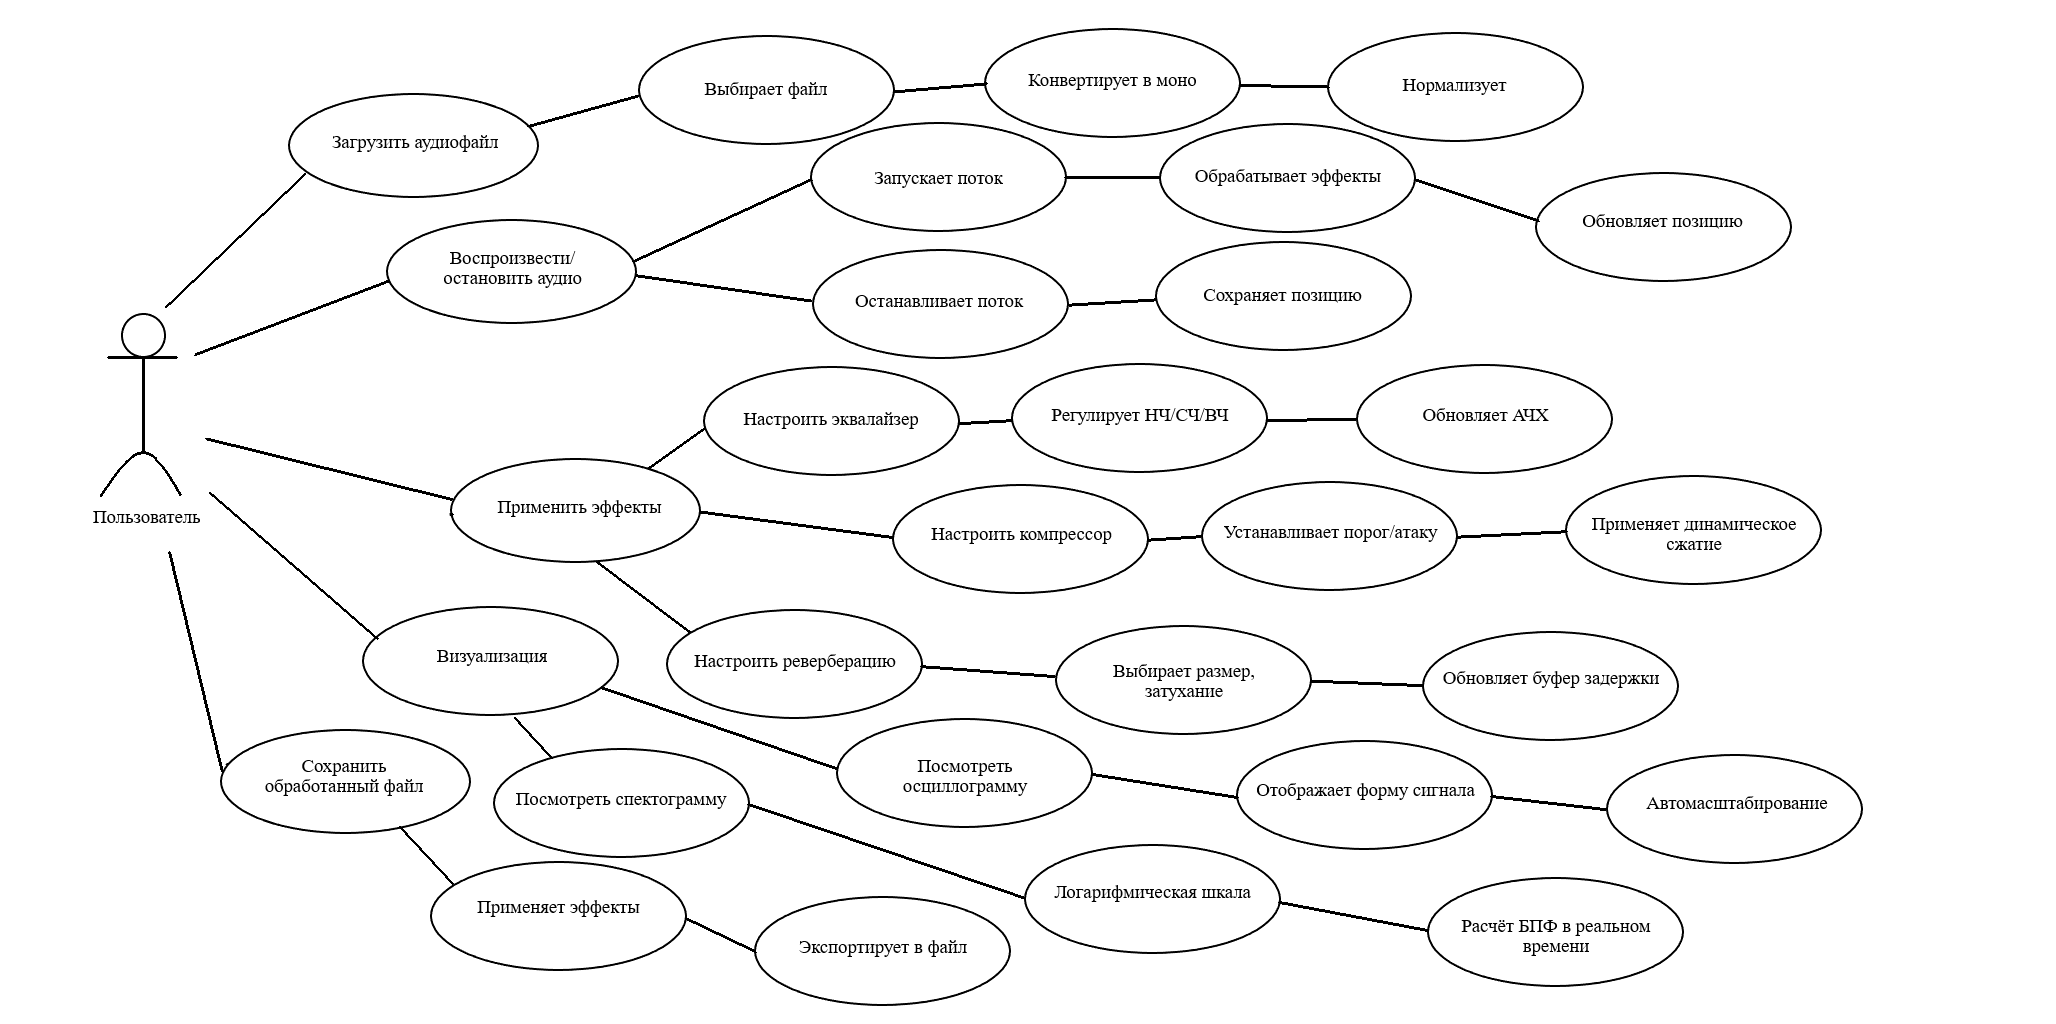
\includegraphics[width=1\linewidth]{DiagramPrec}}
	\caption{Диаграмма прецедентов}
	\label{fig:use_case_diagram}
\end{figure}

\paragraph{Вариант использования «Загрузка аудиофайла»}
Заинтересованные лица и их требования: пользователь хочет загрузить аудиофайл для последующей обработки.

Требования: поддержка форматов (WAV, MP3, OGG, FLAC), автоматическая конвертация в моно, нормализация амплитуды.

Предусловие: приложение запущено, файл существует и доступен для чтения.

Постусловие: аудиоданные загружены в память, форма волны отображена на графике, кнопки "Воспроизвести" и "Сохранить" активированы.

Основной успешный сценарий:
\begin{enumerate}
	\item Пользователь нажимает кнопку "Загрузить".
	\item Открывается диалоговое окно выбора файла.
	\item Пользователь выбирает файл и подтверждает выбор.
\end{enumerate}

\paragraph{Вариант использования «Воспроизведение аудио»}

Заинтересованные лица и их требования: пользователь хочет прослушать загруженный файл с возможностью применения эффектов в реальном времени.

Предусловие: аудиофайл успешно загружен, аудиоустройство вывода доступно.

Постусловие: аудиопоток запущен, графики обновляются в реальном времени.

Основной успешный сценарий:
\begin{enumerate}
	\item Пользователь нажимает кнопку «Воспроизвести».
	\item Система инициализирует аудиопоток.
	\item Callback-функция начинает передавать данные в устройство.
	\item Позиция воспроизведения обновляется каждые 100 мс.
	\item Сигнал и АЧХ отображаются в реальном времени.
\end{enumerate}

\paragraph{Вариант использования «Остановка воспроизведения»}

Заинтересованные лица и их требования: пользователь хочет немедленно прекратить воспроизведение аудио.

Предусловие: идёт воспроизведение аудиофайла.

Постусловие: аудиопоток полностью остановлен, интерфейс обновлен.

Основной успешный сценарий:
\begin{enumerate}
	\item Пользователь нажимает кнопку "Стоп".
	\item Система останавливает воспроизведение аудио.
	\item Текущая позиция фиксируется для возможности дальнейшего продолжения.
\end{enumerate}

\paragraph{Вариант использования «Изменения позиции воспроизведения»}

Заинтересованные лица и их требования: пользователь хочет перемотать аудио на произвольную позицию.

Предусловие: аудиофайл загружен.

Постусловие: текущая позиция воспроизведения изменена, при активном воспроизведении звук продолжается с новой позиции, интерфейс синхронизирован.

Основной успешный сценарий:
\begin{enumerate}
	\item Пользователь перемещает ползунок позиции мышью.
	\item Система пересчитывает позицию.
	\item При воспроизведении поток начинает чтение с новой позиции.
\end{enumerate}

\paragraph{Вариант использования «Применения шумоподавления»}

Заинтересованные лица и их требования: пользователь хочет уменьшить фоновый шум в аудиозаписи для улучшения качества звучания.

Предусловие: файл загружен, кнопка «Шумоподавление» нажата.

Постусловие: выбранный метод шумоподавления и степень обработки применены к аудиопотоку, визуализация обновлена.

Основной успешный сценарий:
\begin{enumerate}
	\item Пользователь активирует кнопку «Шумоподавление».
	\item Выбирает метод шумоподавления из выдвижного списка (спектральное, медианный фильтр, гауссово размытие).
	\item Регулирует интенсивность шумоподавления с помощью knob.
	\item Система применяет выбранный алгоритм с заданной интенсивностью к аудиосигналу.
	\item Обновляется визуализация формы волны и АЧХ.
\end{enumerate}

\paragraph{Вариант использования «Применения эквалайзера»}

Заинтересованные лица и их требования: пользователь хочет настроить частотный баланс (НЧ/СЧ/ВЧ).

Предусловие: файл загружен, вкладка "Эквалайзер" открыта.

Постусловие: параметры эквалайзера применены к аудиопотоку, график АЧХ обновлен.

Основной успешный сценарий:
\begin{enumerate}
	\item Пользователь включает чекбокс «Эквалайзер».
	\item Регулирует ползунки НЧ/СЧ/ВЧ.
	\item Система пересчитывает коэффициент БИХ-фильтров.
	\item Аудиозапись изменяется в соответствии с настройками пользователя.
	\item АЧХ отображается на графике.
\end{enumerate}

\paragraph{Вариант использования «Применения компрессора»}

Заинтересованные лица и их требования: пользователь хочет изменить динамический диапазон аудиосигнала для более равномерного звучания.

Предусловие: аудиофайл успешно загружен, вкладка "Компрессор" открыта.

Постусловие: параметры компрессора применены к аудиопотоку, изменения слышны при воспроизведении.

Основной успешный сценарий:
\begin{enumerate}
	\item Пользователь активирует чекбокс «Компрессор».
	\item Устанавливает диапазон обработки частот для каждого из трёх фильтров.
	\item Устанавливает порог, коэффициент компрессии, время атаки и восстановления, усиление выходного сигнала.
	\item Аудио обрабатывается в режиме реального времени.
\end{enumerate}

\paragraph{Вариант использования «Применения реверберации»}

Заинтересованные лица и их требования: пользователь хочет добавить эффект реверберации к аудиосигналу.

Предусловие: аудиофайл успешно загружен, вкладка "Реверберация" открыта.

Постусловие: эффект реверберации применен к аудиопотоку, буфер реверберации инициализирован с новыми параметрами.

Основной успешный сценарий:
\begin{enumerate}
	\item Пользователь активирует чекбокс "Реверберация".
	\item Пользователь регулирует параметры: уровень эффекта, исходный звук, размер комнаты, затухание.
	\item Аудио обрабатывается в режиме реального времени.
\end{enumerate}	

\paragraph{Вариант использования «Сохранение обработанного файла»}

Заинтересованные лица и их требования: пользователь хочет экспортировать результат с примененными эффектами.

Предусловие: файл загружен, эффекты настроены.

Постусловие: файл сохранен на диск в выбранном формате.

Основной успешный сценарий:
\begin{enumerate}
	\item Пользователь нажимает "Сохранить".
	\item Открывается диалог выбора формата (WAV/MP3) и пути.
	\item Пользователь выбирает формат, путь и название файла.
	\item Система применяет выбранные эффекты, экспортирует файл.
	\item Файл успешно сохранён на диске.
\end{enumerate}		

\paragraph{Вариант использования «Визуализация данных»}

Заинтересованные лица и их требования: пользователь хочет видеть графическое представление аудиосигнала.

Предусловие: аудиофайл загружен и идет воспроизведение.

Постусловие: графики формы волны и АЧХ отображаются и обновляются в режиме реального времени.

Основной успешный сценарий:
\begin{enumerate}
	\item Пользователь нажимает «Воспроизвести».
	\item Система отображает графики формы волны и АЧХ.
\end{enumerate}	

%--------------------------------------------------------------------------------------------------------

\subsection{Требования пользователя к интерфейсу приложения}

Приложение должно иметь следующие основные функции:
\begin{enumerate}
	\item Основные элементы управления - кнопки управления воспроизведением: "Загрузить", "Воспроизвести", "Стоп", "Сохранить". Ползунок позиции воспроизведения, точное позиционирование, индикатор текущей позиции в формате MM:SS / MM:SS.
	\item Визуализация аудио - два синхронизированных графика: верхний график формы волны и нижний график амплитудно-частотной характеристики. Подписи осей с единицами измерения (амплитуда, частота).
	\item Кнопка "Шумоподавление" с двумя положениями: активно/неакитвно, выплывающий список с выбором метода, регулировка интенсивности шумоподавления.
	\item Панель эффектов (вкладки):
	\begin{enumerate}
		\item Эквалайзер - Три ползунка с подписями: низкие частоты (150Hz): ±24 дБ, средние частоты (1kHz): ±24 дБ, высокие частоты (5kHz): ±24 дБ. Чекбокс активации эффекта.
		\item Компрессор - ползунки параметров: порог: -60..0 дБ, соотношение: 1..20, атака: 1..500 мс, восстановление: 10..2000 мс, усиление: 0..24 дБ. Панель отображения диапазонов изменения и применения параметров, а так же ползунки настройки и регулировки диапзаонов. Чекбокс активации эффекта. 
		\item Реверберация: ползунки параметров: уровень эффекта: 0..1, сухой сигнал: 0..1, размер помещения: 0.1..2.0, затухание: 0.1..0.9. Чекбокс активации эффекта.
	\end{enumerate}	
	\item Обратная связь и состояние: индикатор загрузки при обработке файлов. Всплывающие уведомления об ошибках: при неудачной загрузке файла, при проблемах с аудиоустройством, при ошибках сохранения. Изменение состояния кнопок: "Воспроизвести" активна только при загруженном файле, "Стоп" активна только во время воспроизведения, "Сохранить" активна только после загрузки файла.
	\item Производительность: задержка отклика интерфейса не более 100 мс, плавная анимация графиков без рывков, минимальное потребление ресурсов в фоновом режиме.
\end{enumerate}	

\subsubsection{Нефункциональные требования к программно-информационной системе}

\paragraph{Требования к надёжности}

В процессе работы аудио-процессора могут возникнуть следующие аварийные ситуации:
\begin{itemize}
	\item потеря доступа к аудиоустройству в связи с его отключением, изменением системных настроек звука или конфликтом с другим приложением;
	\item попытка загрузки повреждённого или неподдерживаемого аудиофайла с несовместимым форматом, битрейтом или частотой дискретизации;
	\item неожиданное прекращение работы из-за нехватки системных ресурсов при обработке объёмных файлов или одновременном применении нескольких ресурсоёмких эффектов;
	\item ошибки в работе эффектов обработки звука, приводящие к искажению аудиосигнала или сбоям в воспроизведении.
\end{itemize}

Приложение должно автоматически определять доступные аудиоустройства и переключаться между ними при потере соединения с текущим устройством. В случае невозможности восстановления подключения система должна сохранять возможность обработки звука без функции воспроизведения с уведомлением пользователя о возникшей проблеме.

Для работы с аудиофайлами приложение должно проверять их целостность и соответствие поддерживаемым форматам перед загрузкой, а также автоматически выполнять необходимые преобразования (нормализацию, конвертацию в моно, приведение к стандартной частоте дискретизации). При обнаружении критических ошибок в файле пользователь должен получить понятное сообщение о проблеме с указанием конкретной причины.

Для предотвращения аварийного завершения из-за нехватки ресурсов система должна контролировать использование оперативной памяти и процессорного времени, ограничивать размеры буферов обработки и корректно завершать работу при приближении к предельным значениям. Все параметры эффектов и текущее состояние обработки должны сохраняться даже при аварийном завершении работы.

При возникновении ошибок в работе эффектов обработки звука система должна автоматически сбрасывать параметры эффектов к безопасным значениям, сохраняя при этом возможность дальнейшей работы. Все критические ошибки должны фиксироваться в системном логе с указанием времени возникновения, типа ошибки и состояния системы на момент сбоя.

\paragraph{Требования к безопасности}

Требования к приложению:
\begin{enumerate}
	\item Перед загрузкой файла, система должна проверять формат и корректность заголовков. При обнаружении повреждённых данных программа будет выводить ошибку без попытки обработки.
	\item Для безопасности управления памятью и ресурсами необходима изоляция обработки аудио, то есть каждый эффект будет применяться в отдельном потоке с контролем потребления ресурсов и будет ограничен буфе. Так же потребуется очистка временных данных, чтобы после завершения обработки или при ошибке все промежуточные буферы будут очищаться.
	\item Для защиты от вирусов применится проверка структуры файлов, анализ сигнатуры файла перед декодированием, ограничение максимальной длительности обрабатываемого аудио.
	\item Пользовательские настройки будут проверятся перед применением, а недопустимые значения автоматически скорректируются до ближайших безопасных.
	\item При завершении работы, приложение будет останавливать все потоки, освобождать аудиоустройства.
\end{enumerate}

\paragraph{Требования к программному обеспечению}

Для реализации программы будет использоваться язык программирования Python и библиотеки: NumPy, SciPy, PyDub, SoundDevice, Matplotlib, Numba.

Для работы приложения требуется Windows 10/11 (64-bit)

\paragraph{Требования к аппаратному обеспечению}

Минимальная конфигурация:

Центральный процессор с количеством ядер от 2 и выше с тактовой частотой от 2.0 ГГц. Поддержка инструкций SSE4.2. Оперативная память - 4 ГБ. 100 МБ свободного места для установки. Поддержка ASIO/WASAPI для профессионального использования.

\subsubsection{Требования к оформлению документации}

Разработка программной документации и программного изделия должна производиться согласно ГОСТ 19.102-77 и ГОСТ 34.601-90. Единая система программной документации.
\section{Технический проект}

\subsection{Общая характеристика решения задачи}

Задача дипломного проекта заключается в разработке программного аудиопроцессора — универсального программного комплекса для обработки аудиосигналов в реальном времени на персональном компьютере. Процессор реализует цепочку современных аудиоэффектов с возможностью гибкой настройки, а также поддерживает многополосную обработку сигнала, что позволяет применять различные параметры эффектов к разным частотным диапазонам.

Разработка аудиопроцессора, способного выполнять обработку аудиосигнала с применением эквализации, многополосной компрессии, реверберации и шумоподавления.

Входные данные:
\begin{itemize}
	\item аудиосигнал в виде цифрового потока; 
	\item настройки эффектов, задаваемые пользователем (параметры эквалайзера, компрессора, реверберации и шумоподавления).
\end{itemize}

Выходные данные:
\begin{itemize}
	\item обработанный аудиосигнал, выводимый на устройство воспроизведения или сохраняемый в файл; 
	\item возможность мониторинга и визуализации параметров обработки в виде отображения формы волны или АЧХ.
\end{itemize}

\subsection{ Описание используемых технологий и языков программирования}

Для разработки аудиопроцессора был выбран язык программирования Python, что обусловлено рядом ключевых факторов:
\begin{enumerate}
	\item Простота и читаемость кода. Синтаксис Python близок к псевдокоду, что облегчает понимание и сопровождение проекта, а также позволяет быстро экспериментировать с алгоритмами обработки звука.
	\item Широкий набор библиотек для цифровой обработки сигналов. Python обладает мощными библиотеками (NumPy, SciPy, pydub и др.), которые предоставляют готовые инструменты для работы с аудиоданными, фильтрами, преобразованиями и другими DSP-операциями. Это значительно ускоряет разработку и повышает надежность кода.
	\item Возможность оптимизации производительности. Для повышения скорости вычислений в критичных местах применяется JIT-компиляция с помощью Numba, что позволяет добиться близкой к нативной производительности без перехода на более низкоуровневые языки.
	\item Поддержка многопоточности и асинхронной обработки. В проекте используется ThreadPoolExecutor и другие средства стандартной библиотеки для параллельной обработки аудиоданных, что улучшает отзывчивость и снижает задержки при работе в реальном времени.
	\item Гибкость и расширяемость архитектуры. Модульный подход с использованием классов и четким разделением функционала (например, отдельные классы для компрессоров, эквалайзеров и ревербераторов) позволяет легко добавлять новые эффекты и модифицировать существующие.
	\item Активное сообщество и наличие обучающих материалов. Благодаря большому количеству статей, учебников и примеров по цифровой обработке сигналов на Python, разработка и отладка проекта становится более эффективной.
\end{enumerate}

Таким образом, выбор Python и сопутствующих технологий проектирования обусловлен их оптимальным сочетанием простоты, функциональности и производительности, что отвечает требованиям дипломного проекта по созданию программного аудиопроцессора с возможностью обработки в реальном времени и расширяемой архитектурой.

В коде используются следующие библиотеки Python:
\begin{itemize}
	\item NumPy - обеспечивает высокопроизводительные вычисления с многомерными массивами, что критично для обработки аудиоданных, представленных в виде временных рядов;
	\item SciPy - используется для реализации цифровых фильтров (эквалайзер), БПФ (анализ спектра) и других математических операций;
	\item PyDub - библиотека для работы с аудиофайлами, предоставляющая: простые методы загрузки и сохранения в форматах WAV, MP3, OGG, FLAC, базовые операции, такие как обрезка, наложение, изменение громкости, конвертация частоты дискретизации, интеграцию с FFmpeg для поддержки дополнительных кодеков;
	\item Soundfile используется для чтения и записи аудиофайлов различных форматов, обеспечивая удобный доступ к аудиоданным на диске, позволяет загружать исходные аудиозаписи и сохранять результаты обработки без потери качества;
	\item SoundDevice - обеспечивает низкоуровневый доступ к аудиоустройствам через PortAudio. Ключевые функции: воспроизведение и запись в реальном времени с минимальной задержкой, поддержка ASIO, WASAPI, Core Audio для профессиональных аудиоинтерфейсов, гибкая настройка параметров потока: частота дискретизации, размер буфера, количество каналов;
	\item Matplotlib - используется для визуализации аудиоданных: построение осциллограмм (форма сигнала во временной области), отображение АЧХ (амплитудно-частотных характеристик) с логарифмической шкалой, интерактивное обновление графиков в реальном времени;
	\item Threading и concurrent.futures — стандартные библиотеки Python для организации многопоточной и параллельной обработки;
	\item Tkinter - стандартная библиотека Python для создания графического интерфейса. В проекте применяется для: построения основного окна с вкладками (эквалайзер, компрессор, реверберация), реализации интерактивных элементов: ползунки, кнопки, метки, интеграции графиков Matplotlib через FigureCanvasTkAgg;
	\item Numba - JIT-компилятор для оптимизации вычислительно сложных участков кода: ускорение алгоритмов компрессии и реверберации в 5–10 раз, поддержка многопоточности.
\end{itemize}

\subsubsection{Кроссплатформенная библиотека FFmpeg}

FFmpeg — это мощная кроссплатформенная библиотека для обработки мультимедиа, используемая в проекте для работы с аудиофайлами различных форматов. Взаимодействие с FFmpeg осуществляется через обёртку PyDub, что значительно упрощает операции чтения, записи и конвертации аудио.

Основные функции FFmpeg в проекте:
\begin{enumerate}
	\item Поддержка множества аудиоформатов. Позволяет загружать и сохранять файлы в форматах: без сжатия: WAV, AIFF, с потерями: MP3, AAC, OGG, без потерь: FLAC, ALAC. Обеспечивает автоматическое определение кодека при загрузке.
	\item Конвертация аудио: изменение частоты дискретизации, преобразование между форматами, конвертация числа каналов.
	\item Нормализация и обработка. Автоматическая регулировка громкости.
\end{enumerate}

FFmpeg был выбран по рядам преимуществ:
\begin{itemize}
	\item универсальность: поддержка 100+ кодеков и контейнеров;
	\item стабильность: отлаженные алгоритмы декодирования/кодирования;
	\item производительность: оптимизированные нативные библиотеки;
	\item гибкость: Возможность тонкой настройки параметров через командные опции.
\end{itemize}

\subsection{Эффекты}

\subsubsection{Устройство шумоподавления}

Система шумоподавления реализует 4 метода с общим конвейером обработки:
\begin{enumerate}
	\item Спектральное шумоподавление. На основе библиотеки noisereduce, анализирует FFT и подавляет шум в частотной области.
	\item Фильтр Винера. Адаптивная фильтрация во временной области.
	\item Медианный фильтр. Подавление импульсных шумов.
	\item Гауссовский фильтр. Сглаживание высокочастотного шума.
\end{enumerate}

Ключевые особенности:
\begin{itemize}
	\item автодетекция шума: система автоматически запоминает шумовой профиль из первых 2048 сэмплов;
	\item гибкая настройка: регулировка силы подавления (0–100) и выбор метода под тип шума;
	\item потокобезопасность: все операции работают с копиями данных и защищены блокировками;
	\item оптимизация под реальное время: фиксированный размер FFT-окна (512 точек) для минимальной задержки.
\end{itemize}

\subsubsection{Устройство эквалайзера}

Эквалайзер — это устройство или программный алгоритм, предназначенный для корректировки амплитудно-частотной характеристики (АЧХ) звукового сигнала. Он позволяет усиливать или ослаблять определённые частотные диапазоны, изменяя тембр звука. Эквалайзер работает, разделяя входной аудиосигнал на несколько частотных полос (диапазонов), каждая из которых обрабатывается отдельно. После обработки всех полос сигналы складываются, и на выходе получается звук с изменённой частотной характеристикой.

В программе реализован цифровой параметрический эквалайзер, у которого есть три полосы частот, а так же коррекция их по громкости в децибелах. Такие эквалайзеры часто используются в профессиональной звукозаписи и сведении аудио.

Цифровой IIR-фильтр (Биквадратный, на основе Баттерворта)

IIR-фильтр (Infinite Impulse Response — бесконечная импульсная характеристика) — это тип цифрового фильтра, который использует обратную связь, благодаря чему может иметь очень крутые склоны АЧХ при малом порядке.

Биквадратный фильтр (Biquad) — это частный случай IIR-фильтра 2-го порядка, который реализуется с помощью разностного уравнения и часто используется в эквалайзерах из-за своей эффективности.

Фильтр Баттерворта — один из самых популярных типов фильтров, обеспечивающий максимально гладкую АЧХ в полосе пропускания без пульсаций.

Этот эквалайзер обеспечивает:
\begin{itemize}
	\item низкую задержку (важно для реального времени);
	\item минимальные фазовые искажения;
	\item точную обработку частот;
	\item RLock для защиты состояний фильтров.
\end{itemize}

\subsubsection{Устройство многополосного компрессора}

Многополосный компрессор — устройство динамической обработки аудиосигнала, предназначенное для управления динамическим диапазоном звука с разделением сигнала на несколько частотных полос. Основная идея многополосного компрессора заключается в том, что входящий аудиосигнал сначала разделяется на несколько частотных диапазонов с помощью цифровых фильтров, после чего каждая полоса обрабатывается отдельным компрессором с индивидуальными параметрами. Такой подход позволяет более точно и эффективно контролировать динамику звука в каждом частотном диапазоне, сохраняя при этом естественность звучания и минимизируя искажения.

В реализованном компрессоре разделение сигнала осуществляется с использованием цифровых фильтров, которые выделяют низкочастотную, среднечастотную и высокочастотную полосы. Для каждой полосы создаётся отдельный компрессорный блок, реализованный в виде программного модуля, который обрабатывает сигнал независимо от других полос. Каждый из этих блоков имеет собственные настройки ключевых параметров компрессии:
\begin{itemize}
	\item Threshold (порог);
	\item Ratio (коэффициент компрессии); 
	\item Attack (атака);
	\item Release (восстановление);
	\item Knee (характеристика перехода);
	\item Make-up Gain (компенсационное усиление).
\end{itemize}

Реализация JIT-функций для динамического сжатия аудиосигнала.

Пошаговый алгоритм:
\begin{itemize}
	\item вычисление огибающей;
	\item инициализация gain-массива;	
	\item обработка каждого семпла;
	\item преобразование dB в линейное значение:;
	\item экспоненциальное сглаживание;	
	\item применение gain к сигналу.
\end{itemize}

Особенности оптимизации:
\begin{itemize}
	\item векторизованные операции NumPy;
	\item предварительный расчет коэффициентов;
	\item пул потоков для фоновой обработки;
	\item отдельные состояния для каждой полосы;
	\item отсутствие ветвлений в критическом цикле.
\end{itemize}

Порог срабатывания определяет уровень громкости, при превышении которого начинается сжатие сигнала. Коэффициент сжатия задаёт степень уменьшения динамического диапазона, то есть насколько сильно будет снижаться громкость сигналов, превышающих порог. Время атаки регулирует скорость срабатывания компрессора после превышения порога, а время релиза — скорость возврата усиления к исходному уровню после снижения входного сигнала ниже порога, характеристика перехода определяет плавный переход от отсутствия сжатия к активному сжатию сигнала, компенсационное усиление позволяет регулировать сигнал после обработки, чтобы вернуть ему исходную громкость. Эти параметры позволяют гибко настраивать реакцию компрессора на изменения громкости в каждой полосе, обеспечивая плавное и естественное звучание.

В основе алгоритма компрессии лежит вычисление коэффициента усиления (gain reduction), который применяется к аудиосигналу полосы. Этот коэффициент рассчитывается на основе текущего уровня сигнала и параметров компрессии с учётом сглаживания изменения усиления для предотвращения резких артефактов в звуке. Для повышения производительности вычисления оптимизированы с помощью JIT-компиляции (Numba), а обработка полос может выполняться параллельно с использованием многопоточности, что обеспечивает минимальную задержку и возможность работы в реальном времени.

Таким образом, многополосный компрессор, реализованный в проекте, представляет собой совокупность нескольких параллельных компрессоров, каждый из которых отвечает за свой частотный диапазон и имеет независимые настройки. Это обеспечивает высокую гибкость и качество динамической обработки, позволяя адаптировать параметры под особенности конкретного аудиоматериала и задачи. Использование цифровых фильтров для разделения сигнала и оптимизированных алгоритмов компрессии обеспечивает эффективную работу устройства в реальном времени, что соответствует современным требованиям к аудиопроцессорам.

\subsubsection{Устройство реверберации}

FDN (Feedback Delay Network) — это один из самых мощных алгоритмов цифровой реверберации, используемый для создания реалистичных пространственных эффектов. Он основан на множестве линий задержки с обратной связью, образующих сложную сеть, имитирующую отражения в помещении.

Принцип работы:
\begin{itemize}
	\item входной сигнал разделяется на несколько параллельных линий задержки, каждая из которой задерживает сигнал на разное время;
	\item после задержки сигнал проходит через фильтр демпфирования (имитация потери высоких частот);
	\item затем он умножается на коэффициенты матрицы обратной связи, определяющей, какая часть сигнала возвращается в каждую линию;
	\item обновлённый сигнал снова поступает на вход линий задержки;
	\item результирующий реверберационный сигнал формируется как сумма выходов всех линий.
\end{itemize}

Применение JIT-компиляции для создания алгоритма реверберации на основе задержки.

Пошаговый алгоритм:
\begin{itemize}
	\item инициализация буферов;
	\item цикл обработки семплов;
	\item смешивание сигналов;
	\item обновление буфера задержки;
	\item циклическое перемещение по буферу.
\end{itemize}

Ключевые особенности FDN:
\begin{itemize}
	\item реалистичность — лучше имитирует поздние отражения, чем алгоритмы на основе простых задержек;
	\item гибкость — можно настраивать время реверберации, демпфирование и пространственность;
	\item стабильность — ортогональная матрица гарантирует отсутствие бесконечного нарастания.
\end{itemize}

Для обеих функций используются идентичные параметры декоратора: @jit(nopython=True, nogil=True, cache=True), где:
\begin{itemize}
	\item nopython=True - строгий режим (обязательная компиляция);
	\item nogil=True - освобождение GIL для многопоточности;
	\item cache=True - кэширование скомпилированного кода.
\end{itemize}

\subsection{Архитектура программно-информационной системы}

На рисунке \ref{DiagramArch:image} представлена многослойная архитектура системы с чётким разделение ответственности между компонентами.

\begin{figure}[p]  % Разместить на отдельной странице
	\centering
	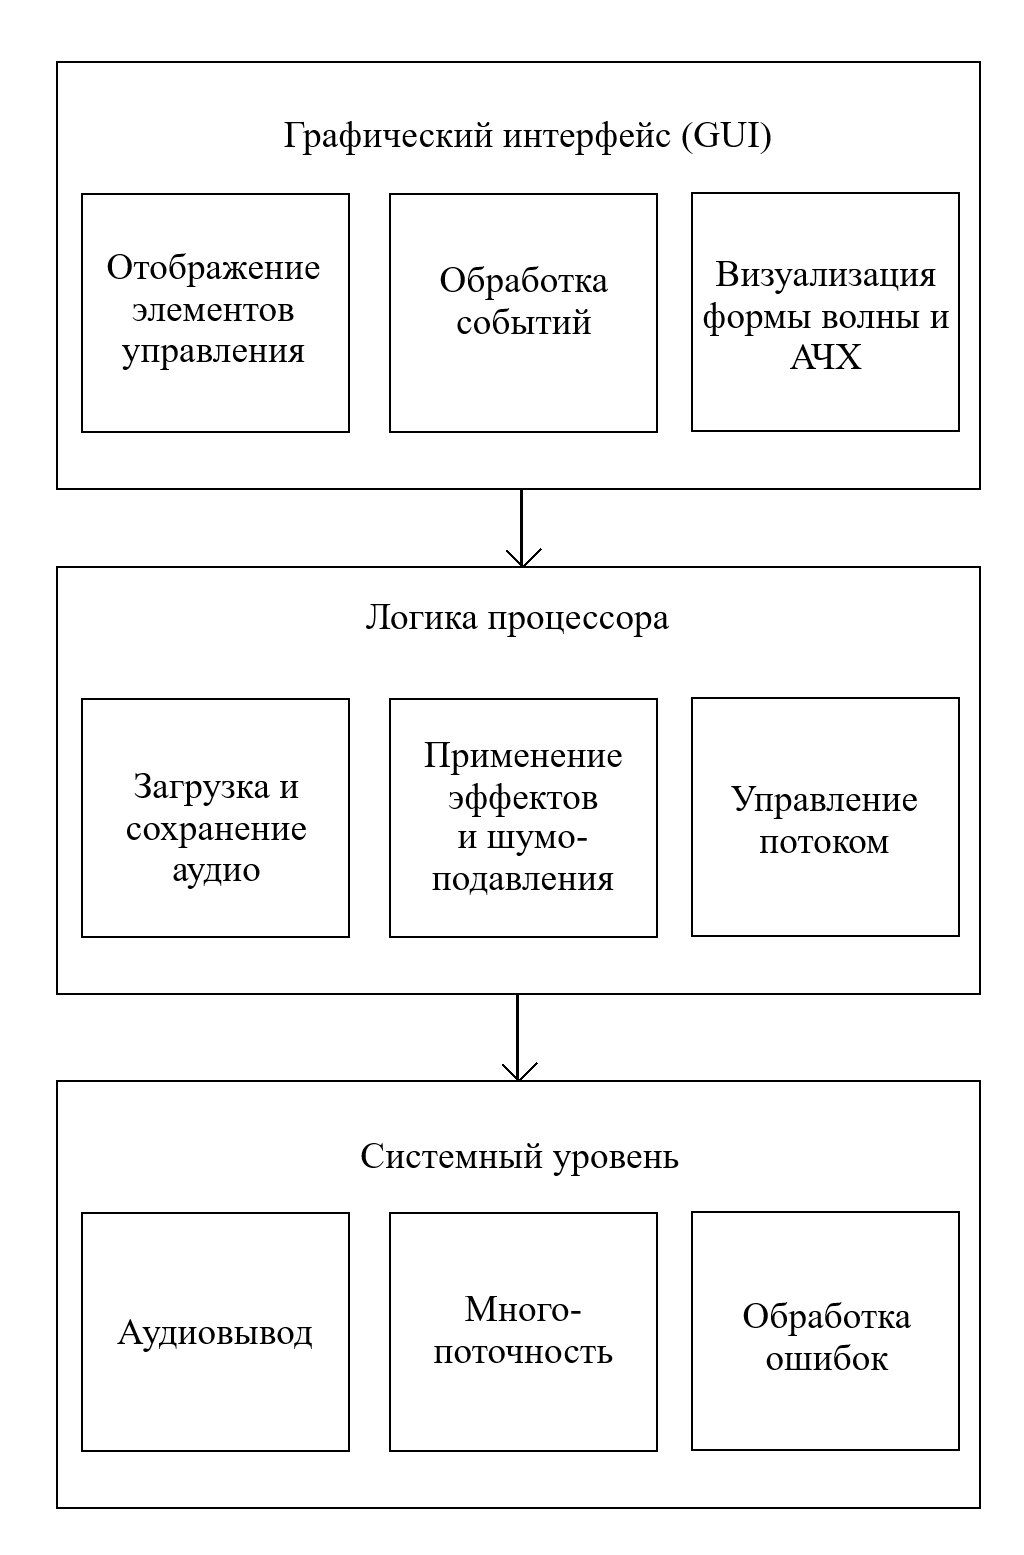
\includegraphics[width=0.8\linewidth]{DiagramArch}
	\caption{Архитектура программно-информационной системы}
	\label{DiagramArch:image}
\end{figure}
\clearpage

\begin{enumerate}
	\item Графический интерфейс отображает элементы управления (кнопки, ползунки, вкладки), визуализирует аудиоданные в реальном времени (Форма волны, АЧХ), обрабатывает пользовательские события (нажатия кнопок, изменение параметров).
	\item Логика процессора отвечает за загрузку/сохранение аудио, чтение файлов через PyDub/FFmpeg, конвертирует в формат float32 для обработки. Применяет эффекты: шумоподавление, эквалайзер (БИХ-фильтры для 8 полос регулировки частот), многополосный компрессор (динамическое сжатие с параметрами), реверберация. Буферизирует данные и синхронизирует позицию воспроизведения.
	\item На уровне системы происходит ввод и вывод аудио, создаётся отдельный поток для обработки аудио и очереди для передачи данных между потоками. Обрабатываются ошибки, перехватываются исключения и логируются в файл.
\end{enumerate}

\begin{itemize}
	\item графический интерфейс включает главное окно, состоящее из кнопок управление воспроизведением и загрузки/сохранения, вкладок эффектов (эквалайзер, компрессор и ревербератор), окна отображение визуализации формы волны и АЧХ;
	\item логика процессора читает и обрабатывает аудиофайлы, применяется выбранные эффекты по очереди, управляет всей работой программы;
	\item системное устройство воспроизводит звук, работает с файлами, открывает и сохраняет их, управляет несколькими задачами одновременно;
	\item вспомогательные модули включают частотный анализ, автоматически регулирует громкость и записывает ошибки и события.
\end{itemize}

Все части программы взаимодействуют между собой по чётким правилам. Когда пользователь меняет настройки, интерфейс передаёт их в модуль обработки, который применяет эффекты и отправляет результат на воспроизведение и отображение. Для плавной работы использовались очереди задач для работы в многопоточном режиме, оптимизирует сложные вычисления для быстрой работы.

\subsection{Архитектура приложения}

Приложение построено по многослойной модульной архитектуре с разделением на логические компоненты, взаимодействующие через четко определенные интерфейсы. В основе лежит ядро обработки аудиосигналов, окруженное графическим интерфейсом, системными сервисами и вспомогательными модулями.
Графический интерфейс реализован на Tkinter и включает:
\begin{itemize}
	\item главное окно (MainWindow) с вкладками для управления эффектами, кнопками воспроизведения/паузы и областью визуализации;
	\item панель эквалайзера (EQPanel) с восьмью ползунками, отображающая АЧХ через Matplotlib;
	\item панель компрессора (CompressorPanel) для настройки порога, сжатия, атаки, восстановления, характеристики перехода, усиления;
	\item панель реверберации (ReverbPanel) для настройки эффект, сухой сигнал, размер комнаты, затухание;
	\item визуализатор спектра (SpectrumAnalyzer), отображающий осциллограмму (форма сигнала) и частотный спектр (БПФ) в реальном времени;
	\item прогресс-бар с управлением позицией воспроизведения и отображением длительности трека.	
\end{itemize}

Логический процессор — центральный модуль, отвечающий за:
\begin{itemize}
	\item загрузку и конвертацию аудио через PyDub (с использованием FFmpeg как бэкенда), включая поддержку WAV, MP3, FLAC;
	\item эквалайзер на БИХ-фильтрах с частотами 50 Гц, 150 Гц, 250 Гц, 500 Гц, 1 кГц, 3 кГц, 7 кГц, 15 кГц;
	\item компрессор с разделением на три диапазона частот, в каждом из которых есть регулировки: treshold, ratio, knee, attack, rrelease, gain;
	\item реверберация на основе алгоритма Schroeder (комбинация линий задержки и FIR-фильтров);
	\item буферизацию данных для плавного воспроизведения и нормализацию уровня сигнала.
\end{itemize}

Системный слой обеспечивает интеграцию с ОС и оборудованием:
\begin{itemize}
	\item аудиопоток (AudioStream) на базе SoundDevice, обрабатывающий ввод/вывод в реальном времени с настройкой latency и sample rate (44.1–192 кГц);
	\item менеджер потоков (ThreadManager) для параллельной обработки (отдельные потоки для: GUI, аудиообработки, визуализации);
	\item файловый менеджер (FileManager) с кэшированием загруженных треков и поддержкой метаданных (ID3-теги).
\end{itemize}

Архитектура обеспечивает масштабируемость (добавление новых эффектов через модули), производительность (JIT-компиляция, многопоточность) и отказоустойчивость (изоляция сбоев в отдельных потоках).

\subsubsection{Многопоточная обработка}

В коде используется несколько потоков для различных задач

Основные потоки класса AudioProcessor:
\begin{enumerate}
	\item Поток обработки аудио (processing\_loop). Основной цикл обработки аудиоданных. Выполняет: обрабатывает аудиоданные из очереди input\_queue, применяет эффекты (эквалайзер, компрессор, реверберацию), отправляет обработанные данные в очередь output\_queue, управляет частотой обновления для минимизации нагрузки на CPU.
	\item Потоки пула исполнителей (ThreadPoolExecutor). Выполнение задач в фоновом режиме. Выполняет: обработку аудио в фоне (process\_in\_background), другие тяжелые вычисления без блокировки основного потока.
	\item Поток обновления позиции воспроизведения. Следит за текущей позицией воспроизведения. Обновляет ползунок и метку времени. Проверяет завершение воспроизведения.
\end{enumerate}

Основные потоки класса AudioApp:
\begin{enumerate}
	\item Поток инициализации приложения (\_background\_init). Инициализирует AudioProcessor. Загружает данные для графиков. Переключается на основной интерфейс после завершения.
	\item Поток загрузки аудио (\_load\_audio\_in\_thread). Загрузка и конвертация аудиофайлов. Чтение файла. Конвертация в моно и нормализация. Передача данных в основной поток.
	\item Поток воспроизведения аудио (через sounddevice.OutputStream). Непрерывная передача аудиоданных на звуковую карту. Вызывает \_audio\_callback для получения новых данных. Обрабатывает ошибки устройства. Останавливается при завершении воспроизведения.
	\item Поток сохранения аудио (\_process\_and\_save\_audio). Сохранение обработанного аудио в файл. Применяет все эффекты к аудио. Конвертирует в выбранный формат. Сохраняет на диск.
	\item Поток обновления интерфейса (update\_gui). Периодическое обновление графиков и элементов управления. Обновляет форму волны и АЧХ (15 FPS). Обновляет позицию воспроизведения (10 FPS). Проверяет состояние воспроизведения.
\end{enumerate}

Для потокобезопасности используются:
\begin{itemize}
	\item threading.RLock для доступа к аудиоданным;
	\item queue.Queue для межпоточного обмена данными;
	\item threading.Event для управления состоянием;
	\item after в Tkinter для обновления GUI из основного потока.
\end{itemize}

\subsection{Проект данных программно-информационной системы}

Система оперирует тремя основными категориями данных: входными, промежуточными и выходными. Входные данные включают аудиофайлы в форматах WAV, MP3, FLAC и OGG с поддержкой различных характеристик (битность 16-24 бит, частота дискретизации 44.1-192 кГц), а также параметры эффектов, настраиваемые пользователем через графический интерфейс. Для эквалайзера это уровни усиления по восьми полосам (50 Гц, 150 Гц, 250 Гц, 500 Гц, 1 кГц, 3 кГц, 7 кГц, 15 кГц с диапазоном ±24 дБ), для каждого диапазона компрессора — порог срабатывания от -60 до 0 дБ, коэффициент компрессии от 1:1 до 10:1, характеристика перехода от 0 до 100, время атаки от 0.1 до 100 мс, время восстановления от 10 до 1000 мс, усиление от -20 до +20 дБ, для реверберации — соотношение обработанного и исходного сигнала, виртуальный размер помещения, затухание, две регулировки среза верхних и нижних частот, панорамирование.

Промежуточные данные представлены в виде нормализованных аудиобуферов в формате 32-битных чисел с плавающей запятой, организованных как моно- или стереоканальные массивы. Система использует кольцевые буферы для обработки в реальном времени и промежуточные спектральные данные, полученные через быстрое преобразование Фурье с применением оконной функции. Для хранения состояния эффектов используются специализированные структуры: коэффициенты БИХ-фильтров эквалайзера, параметры огибающей компрессора и линии задержки реверберации.

Выходные данные включают обработанные аудиофайлы в выбранных пользователем форматах (WAV с PCM-кодированием или MP3 с переменным битрейтом), сохраняющие исходные параметры частоты дискретизации или конвертируемые к стандартным значениям. Визуализационные данные содержат три основных компонента: осциллограмму последних обработанных сэмплов, частотный спектр с разрешением 8192 точек и амплитудно-частотную характеристику активных фильтров, отображаемую в логарифмическом масштабе от 20 Гц до 20 кГц.

Метаданные системы включают пользовательские пресеты эффектов, содержащие полный набор параметров обработки, историю операций для возможности отмены действий, а также технические лог-файлы с информацией о производительности и ошибках. Все данные передаются между компонентами системы через единый формат аудиоблоков, сопровождаемых метаинформацией о текущих настройках обработки, что обеспечивает согласованность работы многопоточной архитектуры.

\subsubsection{Описание сущностей графического интерфейса}

Графический интерфейс Audio Processor представляет собой комплекс взаимосвязанных визуальных компонентов, объединенных в единое интуитивное пространство. 

Интерфейс поддерживает несколько режимов отображения - компактный для мониторов с малым разрешением, расширенный с дополнительными инструментами анализа для профессиональной работы, и режим презентации с увеличенными элементами управления. Все визуальные компоненты реализованы с учетом эргономики - важные элементы выделены акцентным цветом, соблюдены принципы визуальной иерархии, обеспечена последовательная реакция на пользовательские действия. Особенностью интерфейса является синхронизация всех элементов - изменения параметров эффектов мгновенно отражаются на графиках, а действия пользователя сопровождаются тактильной обратной связью в виде тонких анимационных эффектов.

\subsubsection{Описание сущностей логики процессора}

Основу обработки составляет низкоуровневый модуль, работающий с потоком аудиосэмплов в формате 32-битных чисел с плавающей точкой, обеспечивающий базовые операции нормализации и передискретизации. Система эффектов построена вокруг трех ключевых процессоров: эквалайзер реализует трехполосную фильтрацию через каскад БИХ-фильтров с настраиваемыми частотами среза и коэффициентами усиления, компрессор отвечает за компрессию сигнала с алгоритмами расчета огибающей и адаптивными параметрами атаки/восстановления, а ревербератор генерирует реверберацию через комбинацию линий задержки с регулируемыми параметрами затухания.

Поток данных управляется специализированным менеджером маршрутизации, который обеспечивает передачу аудиоблоков между модулями с минимальной задержкой, используя кольцевые буферы и механизм синхронизации для многопоточной работы. Состояние системы отслеживает активные эффекты, параметры обработки и текущий режим работы (реальное время/оффлайн обработка), предоставляя единый интерфейс для управления конвейером обработки. 

\subsubsection{Описание сущностей системного уровня}

Системная архитектура приложения построена на нескольких ключевых компонентах, обеспечивающих интеграцию с операционной средой и аппаратными ресурсами. Центральным элементом выступает абстрактный слой взаимодействия с аудиодрайверами, реализующий поддержку ASIO, WASAPI и Core Audio через единый кроссплатформенный API. Для управления устройствами ввода-вывода используется DeviceManager, который автоматически обнаруживает доступные аудиоинтерфейсы, анализирует их характеристики и предоставляет унифицированный интерфейс для работы с ними.

Файловая подсистема основана на компоненте, объединяющем возможности стандартных Python-библиотек для работы с файлами и мощь FFmpeg для обработки мультимедиа. Этот модуль включает кэширующий механизм для ускорения повторного доступа к аудиофайлам и систему контроля целостности данных. 

Многопоточная архитектура координируется центральным диспетчером задач, который создает и управляет тремя основными типами потоков: высокоприоритетным аудиопотоком реального времени, фоновыми рабочими потоками для обработки эффектов и служебными потоками для визуализации и логирования.

\subsection{Проектирования пользовательского интерфейса}

Центральное место занимает динамическая визуализация аудиопотока - двойной дисплей с синхронизированными осциллограммой и АЧХ, выполненный в темной цветовой гамме с акцентными элементами салатового цвета для выделения ключевых параметров сигнала. Основная рабочая область: верхняя треть экрана отведена под графики, центральная часть содержит компактные панели эффектов с интуитивными регуляторами, а нижний сектор занимает расширенная панель транспорта с профессиональными элементами управления.

Навигационная система реализована через адаптивную панель вкладок с контекстно-зависимыми элементами управления - при выборе конкретного эффекта (эквалайзер, компрессор, реверберация) нижняя панель автоматически наполняется соответствующими регуляторами, сохраняя при этом быстрый доступ к основным функциям. Все элементы управления спроектированы с учетом тактильного взаимодействия - ползунки имеют выраженные рифленые ручки с магнитными точками для часто используемых значений, кнопки обладают трехступенчатой визуальной обратной связью (покой, наведение, нажатие), а переключатели сопровождаются мягкими анимационными переходами.


\ifПрактика{}\else{
   \section{Рабочий проект}

\subsection{Классы, используемые при разработке приложения}

\subsubsection{Класс AudioProcessor}

Класс для обработки аудиосигналов. Реализует эффекты (эквалайзер, компрессор, реверберацию) и предоставляет методы для их настройки и применения к аудиоданным. Поддерживает многопоточную обработку и потоковое воспроизведение.
 
Основные методы:
\begin{enumerate}
	\item \_\_init\_\_(self): инициализация параметров и буферов. Реализация: создает RLock-блокировки для потокобезопасности (self.lock, self.position\_lock), инициализирует эффекты через \_init\_effects(), включая параметры эквалайзера (eq\_params), компрессора (compressor\_params), реверберации (reverb\_params), настраивает пул потоков (ThreadPoolExecutor) для фоновых задач.
	\item load\_audio(self, filename: str): загрузка аудиофайла через pydub. Реализация: конвертирует файл в моно/стерео, нормализует амплитуду, сохраняет данные как NumPy-массив в self.audio\_data.
	\item process\_in\_background(): асинхронная обработка аудио в отдельном потоке. Применение эффектов к большим аудиоблокам без зависания GUI. Обработка в ThreadPoolExecutor (пул из 2 потоков).
	\item processing\_loop(): основной цикл обработки аудио в фоне. Работает в отдельном потоке (threading.Thread). Использует очереди (input\_queue, output\_queue) для потокобезопасного обмена данными. Ограничивает нагрузку на CPU (через time.sleep при высокой загрузке).
	\item apply\_all\_effects(self, data: np.ndarray): применяет цепочку эффектов к аудиоблоку. Порядок обработки: шумоподавление (apply\_noise\_reduction), эквалайзер (apply\_eq), компрессор (apply\_compressor), реверберация (apply\_reverb). Оптимизация: использует numba.jit для apply\_compressor\_numba и apply\_reverb\_numba, буферизация состояний фильтров.
	\item apply\_noise\_reduction(self, data: np.ndarray): применяет алгоритм шумоподавления к аудиоданным. Поддерживает несколько методов шумоподавления: spectral - спектральное шумоподавление (использует noisereduce), wiener - фильтр Винера, median - медианный фильтр, gaussian - гауссовский фильтр.
	\item apply\_eq(self, data: np.ndarray). Для каждой полосы эквалайзера (50Hz, 150Hz, ... 15kHz): рассчитывает БИХ-фильтр через scipy.signal.butter, Применяет фильтр с учетом усиления через lfilter.
	\item apply\_multiband\_compressor(self, data: np.ndarray). Логика работы: разделяет сигнал на 3 полосы (НЧ/СЧ/ВЧ) через \_apply\_bandpass и для каждой полосы: вычисляет огибающую и применяет пороговое сжатие с учётом атаки/спада. Возвращает сумму обработанных полос.
	\item apply\_reverb(self, data: np.ndarray). Логика работы: смешивает входной сигнал с задержанной версией, регулирует ослабление задержанного сигнала (damping) и фильтруется (ФНЧ/ФВЧ), результат смешивается с исходным сигналом по параметрам wet и dry.
\end{enumerate}

\subsubsection{Класс AudioApp}

Главный класс GUI приложения. Содержит интерфейс для управления аудиоэффектами, визуализации сигналов и взаимодействия с AudioProcessor. Реализует загрузку/сохранение файлов и управление воспроизведением.

Основные методы:
\begin{enumerate}
	\item \_\_init\_\_(self): создает главное окно Tkinter с вкладками (ttk.Notebook), настраивает стили (ttk.Style) для основной темы приложения, запускает фоновую инициализацию процессора через \_start\_background\_init.
	\item \_create\_main\_interface(self): кнопки загрузки, управления воспроизведением, сохранением, применением шумоподавления, ползунок позиции, два графика через FigureCanvasTkAgg, вкладки с регуляторами для эквалайзера, компрессора, реверберации.
	\item update\_gui(self): основной метод обновления графического интерфейса. Выполняет: обновление позиции воспроизведения (10 FPS), обновление графиков сигналов (15 FPS), проверку состояния воспроизведения, обработку очереди сообщений для визуализации.
	\item \_audio\_callback(self, outdata, frames, time\_info, status): получает аудиоблок из processor.apply\_all\_effects(), отправляет данные в outdata для звуковой карты, помещает сэмплы в plot\_queue для визуализации.
\end{enumerate}

\subsubsection{Класс Knob}

Кастомный виджет регулятора в виде крутящейся ручки, реализованный на tk.Canvas. Позволяет интерактивно изменять числовые параметры с помощью вращения мыши и обеспечивает визуальную обратную связь.

Основные методы:
\begin{enumerate}
	\item \_on\_drag(self, event): обрабатывает перемещение мыши, вращая регулятор.
	\item \_update\_pointer(self, angle): перерисовывает стрелку на Canvas.
\end{enumerate}

\subsubsection{Класс App}

Главный класс-обёртка приложения, отвечающий за инициализацию среды, обработку ошибок и запуск основного GUI (AudioApp). Реализует проверку зависимостей, глобальный обработчик исключений и настройку приоритетов процессов для стабильной работы аудио.

Основной метод main(): настраивает обработчик исключений (sys.excepthook), проверяет зависимости (check\_dependencies()), создает экземпляр AudioApp и запускает главный цикл.

\subsection{Описание элементов интерфейса пользователя}

На рисунке \ref{InterProg:image} интерфейс программы при запуске.

\begin{enumerate}
	\item Окно отображения графика формы волны.
	\item Окно отображения графика АЧХ.
	\item Кнопка загрузки аудиофайла (активно).
	\item Кнопка воспроизведения аудио (активно).
	\item Кнопка остановки аудио (неактивна).
	\item Кнопка сохранения аудио (неактивно).
	\item Кнопка шумоподавления (неактивно).
	\item Knob регулировки уровня шумоподавления.
	\item Отображение процентов воздействия шумподавления на аудио.
	\item Слайдер отслеживания и управление временем воспроизведения.
	\item Время аудио нынешнее/полное.
	\item Активная вкладка открытого окна эквалайзера.
	\item Неактивная вкладка закрытого окна компрессора.
	\item Неактивная вкладка закрытого окна реверберации.
	\item Чекбокс включения эквалайзера.
	\item Слайдер регулировки уровня частоты 50 Гц с подписанным снизу параметром настройки.
	\item Слайдер регулировки уровня частоты 150 Гц с подписанным снизу параметром настройки.
	\item Слайдер регулировки уровня частоты 250 Гц с подписанным снизу параметром настройки.
	\item Слайдер регулировки уровня частоты 500 Гц с подписанным снизу параметром настройки.
	\item Слайдер регулировки уровня частоты 1 кГц с подписанным снизу параметром настройки.
	\item Слайдер регулировки уровня частоты 3 кГц с подписанным снизу параметром настройки.
	\item Слайдер регулировки уровня частоты 7 кГц с подписанным снизу параметром настройки.
	\item Слайдер регулировки уровня частоты 15 кГц с подписанным снизу параметром настройки.
\end{enumerate}

\begin{figure}[ht]
	\center{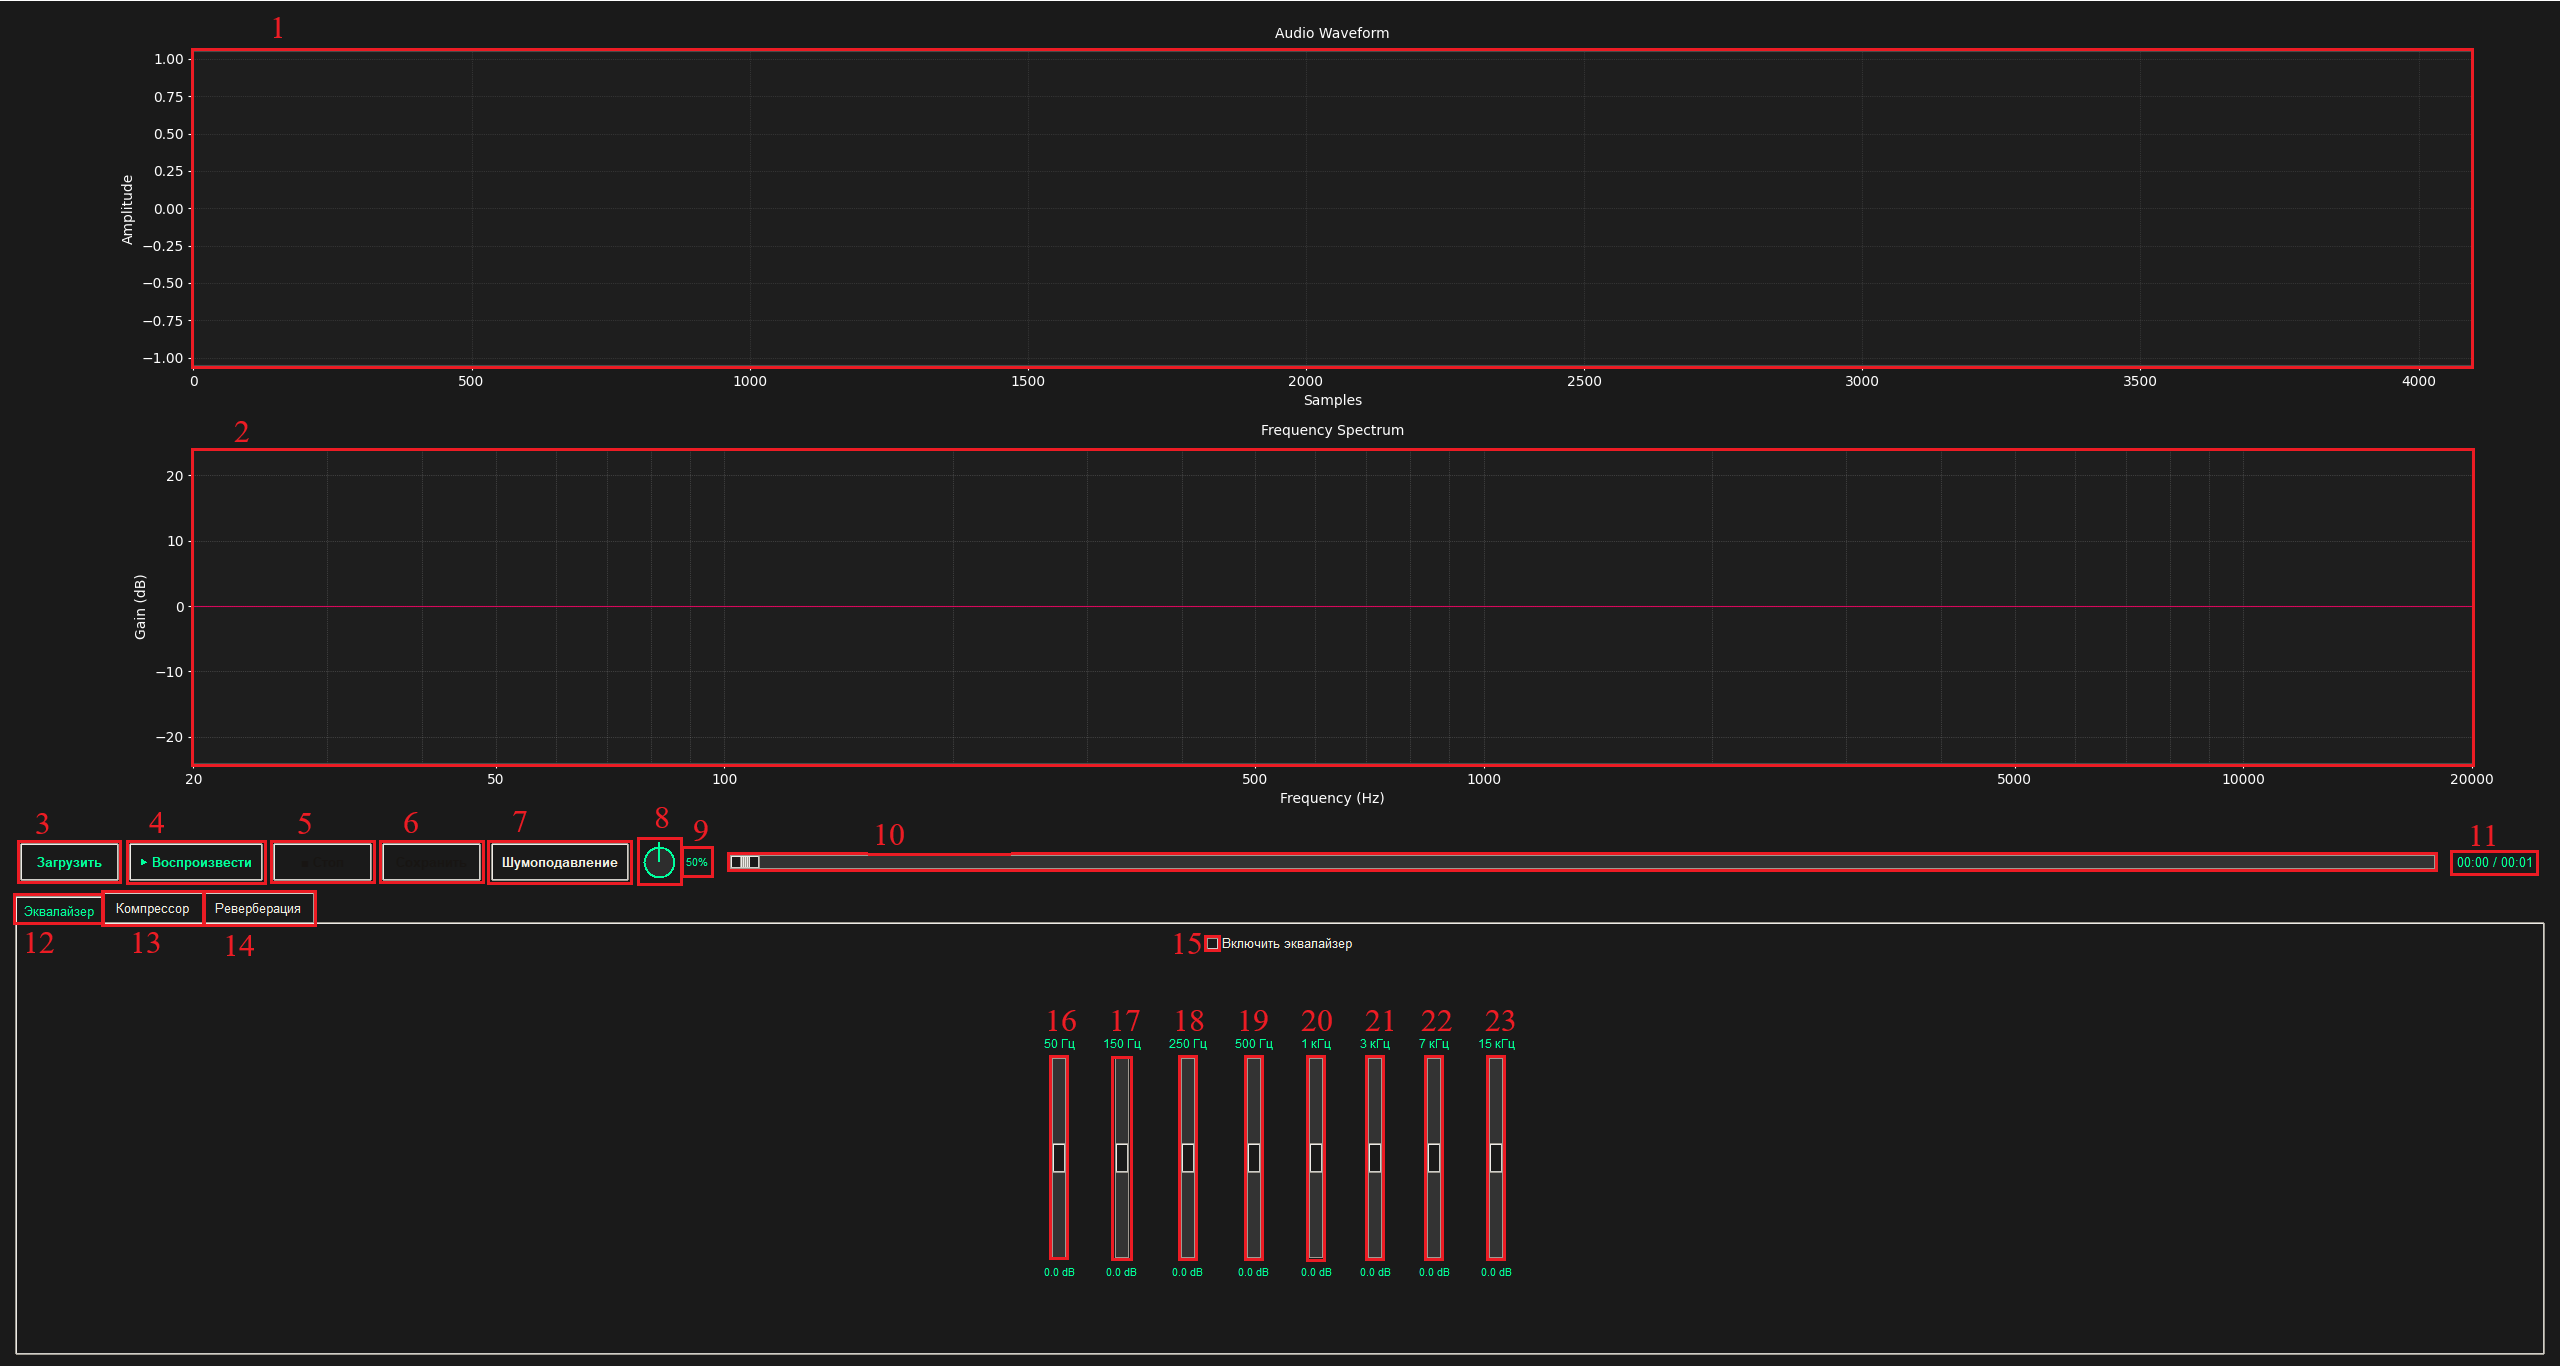
\includegraphics[width=1\linewidth]{InterProg}}
	\caption{Интерфейс приложения при запуске.}
	\label{InterProg:image}
\end{figure}

На рисунке \ref{WindLoad:image} окно загрузки аудиофайла.

\begin{figure}[ht]
	\center{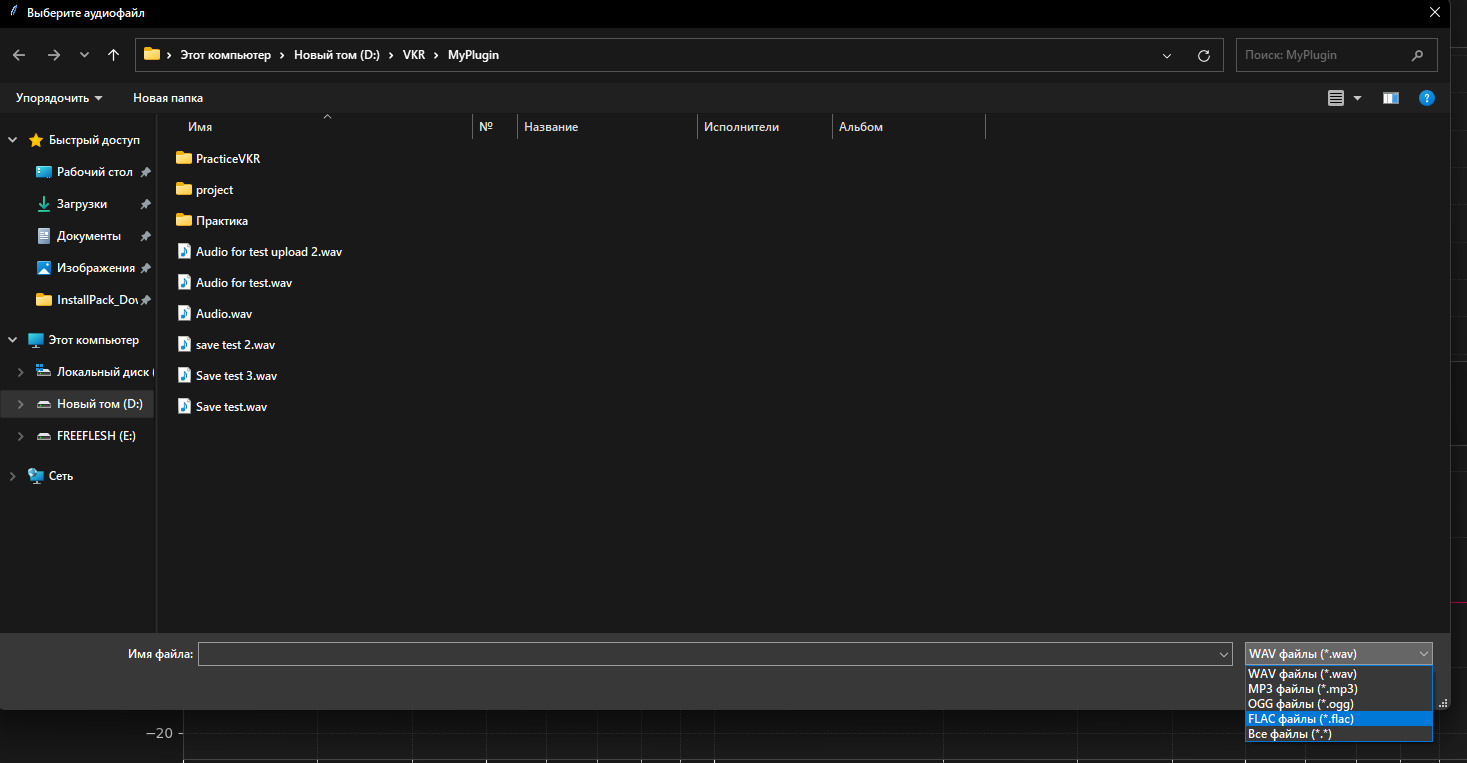
\includegraphics[width=1\linewidth]{WindLoad}}
	\caption{Окно загрузки аудиофайла.}
	\label{WindLoad:image}
\end{figure}

На рисунке \ref{CompWind:image} интерфейс вкладки компрессора.

\begin{enumerate}
	\item Кнопка воспроизведения аудио (неактивно).
	\item Кнопка остановки аудио (активно).
	\item Кнопка сохранения аудио (активно).
	\item Активная кнопка шумоподавления.
	\item Окно регулировки диапазонов обработки частот.
	\item Ползунок регулировки диапазона низких частот.
	\item Ползунок регулировки диапазона высоких частот.
	\item Подпись диапазонов.
	\item Неактивный чекбокс bypass.
	\item Knob регулировки Threshold с подписью значения настройки (аналагично для всех диапазонов).
	\item Knob регулировки Ratio с подписью значения настройки (аналагично для всех диапазонов).
	\item Knob регулировки Knee с подписью значения настройки (аналагично для всех диапазонов).
	\item Knob регулировки Attack с подписью значения настройки (аналагично для всех диапазонов).
	\item Knob регулировки Release с подписью значения настройки (аналагично для всех диапазонов).	
	\item Knob регулировки Gain с подписью значения настройки (аналагично для всех диапазонов).
	\item Чекбокс активного включения компрессора.
	\item Чекбокс активного bypass.
\end{enumerate}

\begin{figure}[ht]
	\center{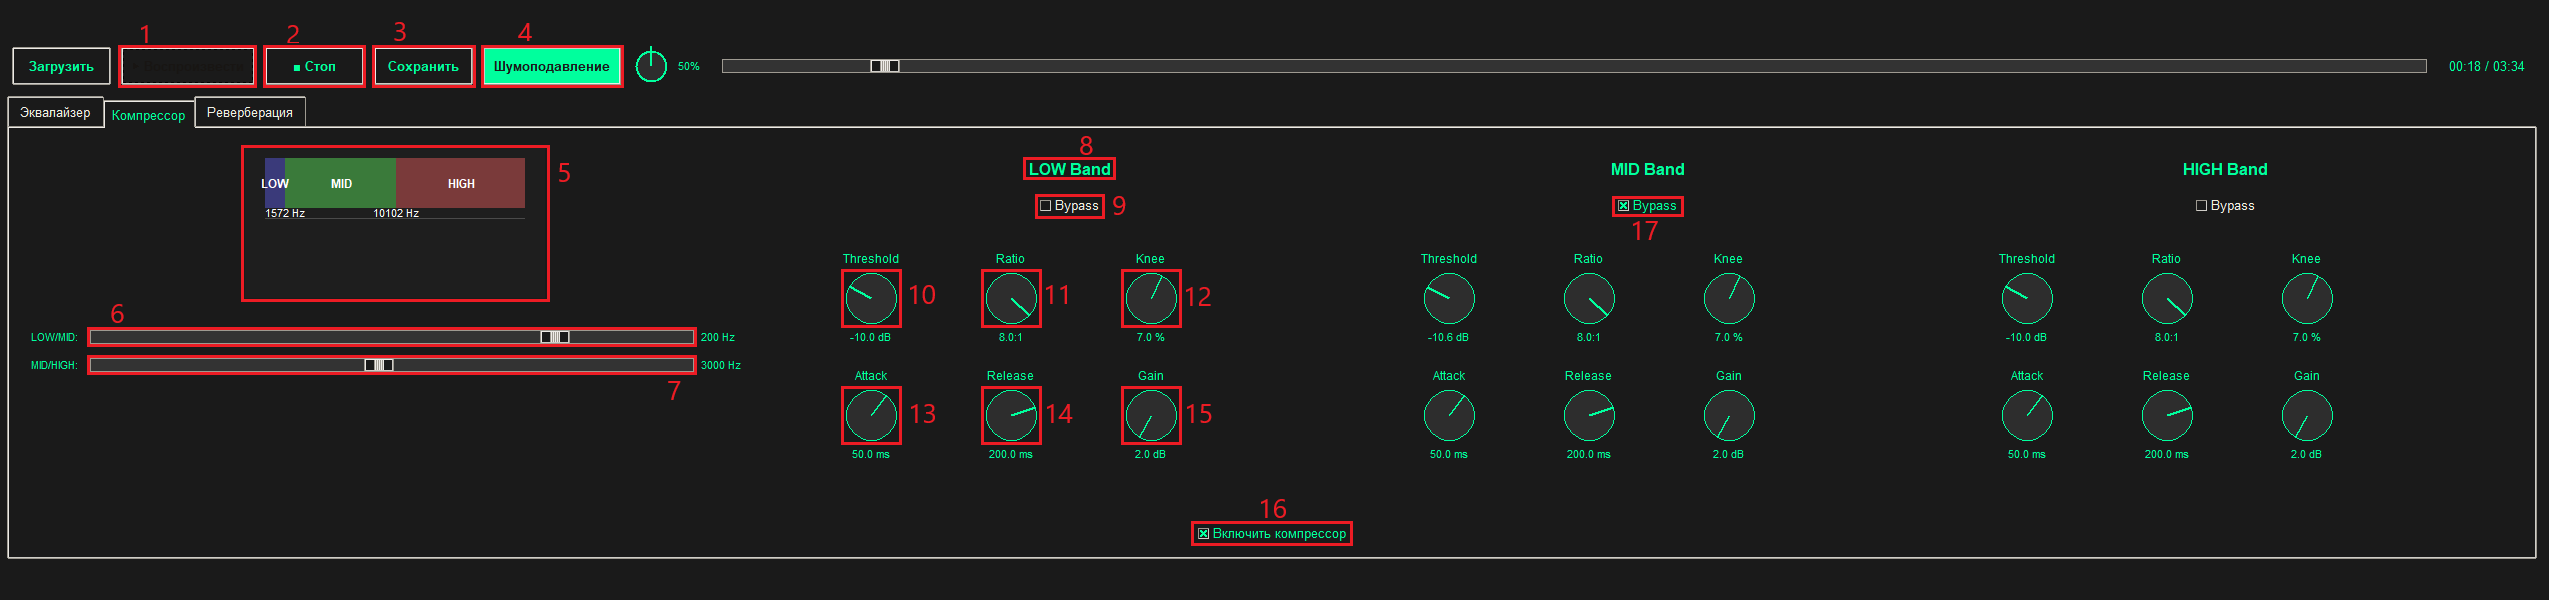
\includegraphics[width=1\linewidth]{CompWind}}
	\caption{Интерфейс вкладки компрессора.}
	\label{CompWind:image}
\end{figure}

На рисунке \ref{ReverbWind:image} интерфейс вкладки реверберации.

\begin{enumerate}
	\item Knob регулировки Wet с подписью значения настройки.
	\item Knob регулировки Dry с подписью значения настройки.
	\item Knob регулировки Size с подписью значения настройки.
	\item Knob регулировки Damping с подписью значения настройки.
	\item Knob регулировки High Cut с подписью значения настройки.
	\item Knob регулировки Low Cut с подписью значения настройки.
	\item Knob регулировки Pan с подписью значения настройки.
	\item Чекбокс активации реверберации (неактивно).
\end{enumerate}

\begin{figure}[ht]
	\center{
\includegraphics[width=1\linewidth]{ReverbWind}}
	\caption{Интерфейс вкладки реверберации.}
	\label{ReverbWind:image}
\end{figure}

На рисунке \ref{SaveWind:image} окно сохранения аудиофайла.

\begin{figure}[ht]
	\center{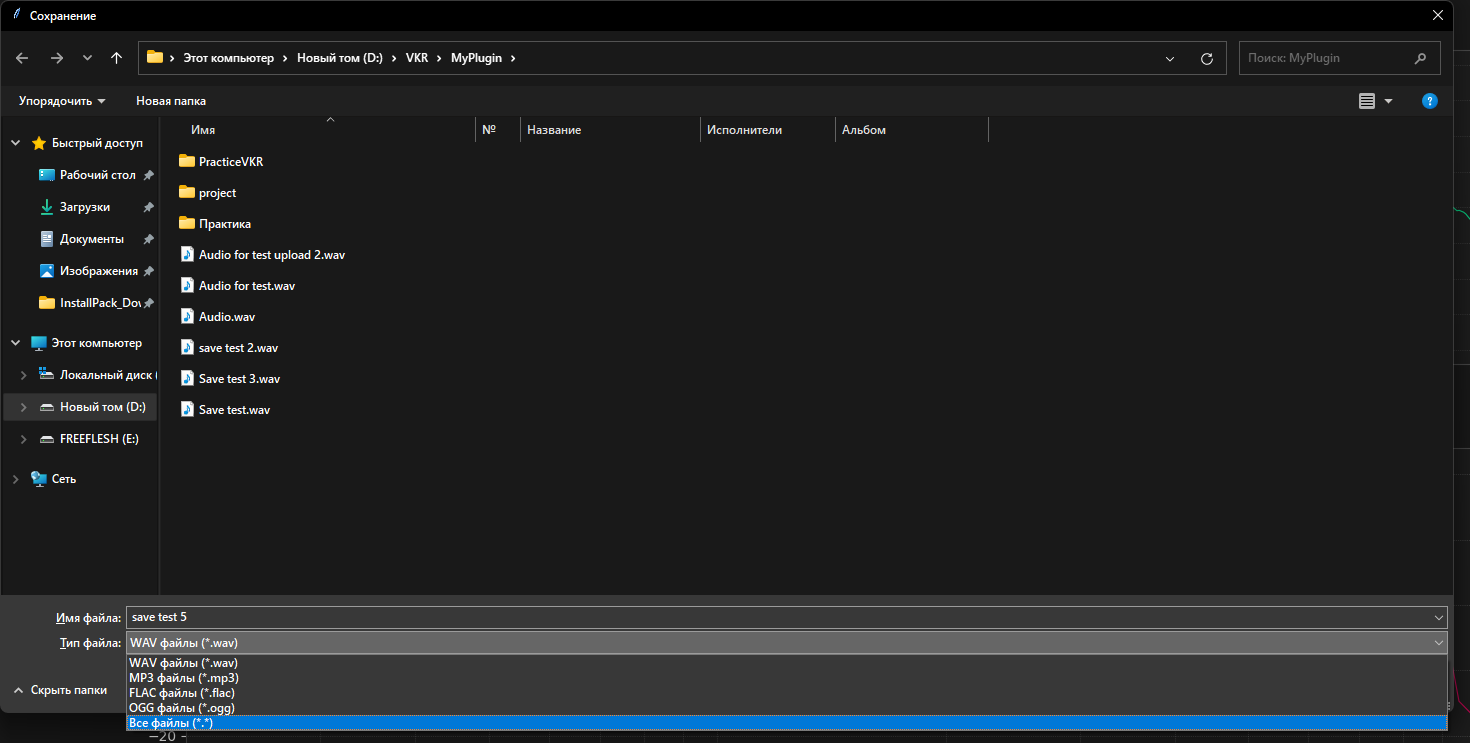
\includegraphics[width=1\linewidth]{SaveWind}}
	\caption{Окно сохранения аудиофайла.}
	\label{SaveWind:image}
\end{figure}

\subsection{Тестирование программно-информационной системы}

Тестирование аудиопроцессора — комплексный процесс, включающий проверку корректности работы всех модулей, качество обработки звука, устойчивость к ошибкам и соответствие требованиям. Для обеспечения высокого качества и надёжности программно-информационной системы необходимо провести как позитивное, так и негативное тестирование с использованием различных методов и сценариев.

\clearpage
\textbf{1) Запуск приложения}

Описание: Пользователь открывает приложение и оно запускается без ошибок и отображает рабочий интерфейс.

На рисунке \ref{LoadingWind:image} загрузка приложения.

\begin{figure}[ht]
	\center{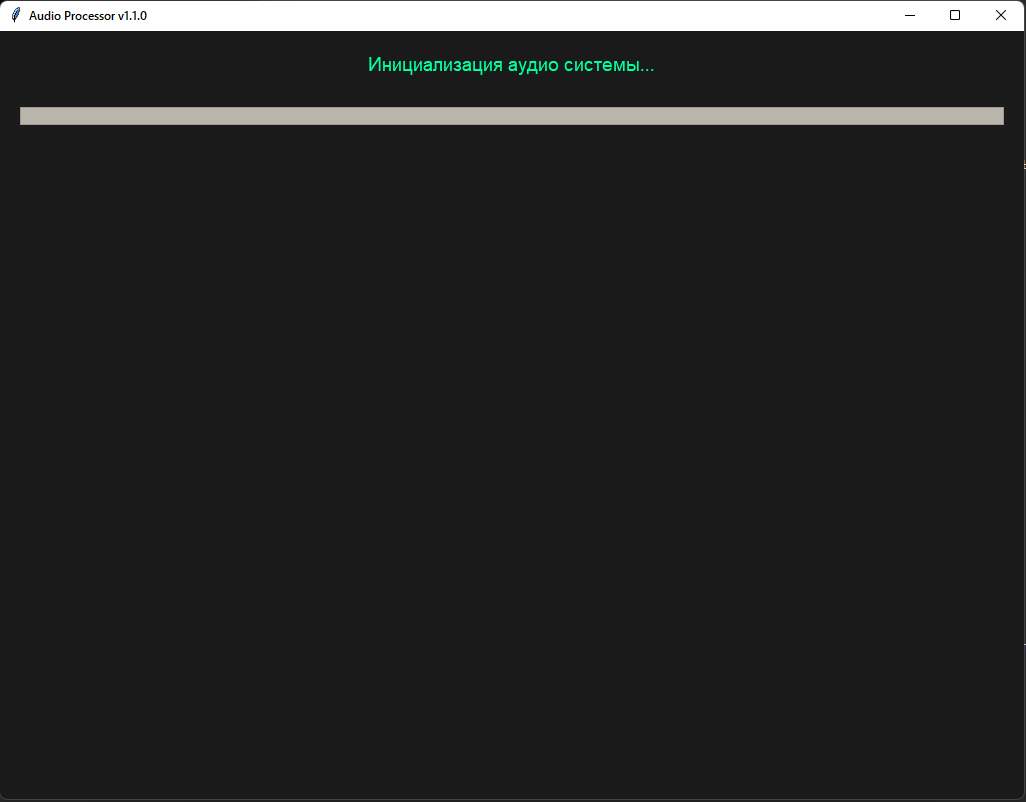
\includegraphics[width=0.8\linewidth]{LoadingWind}}
	\caption{Окно загрузки приложения.}
	\label{LoadingWind:image}
\end{figure}

На рисунке \ref{Interface:image} интерфейс программы.

\begin{figure}[ht]
	\center{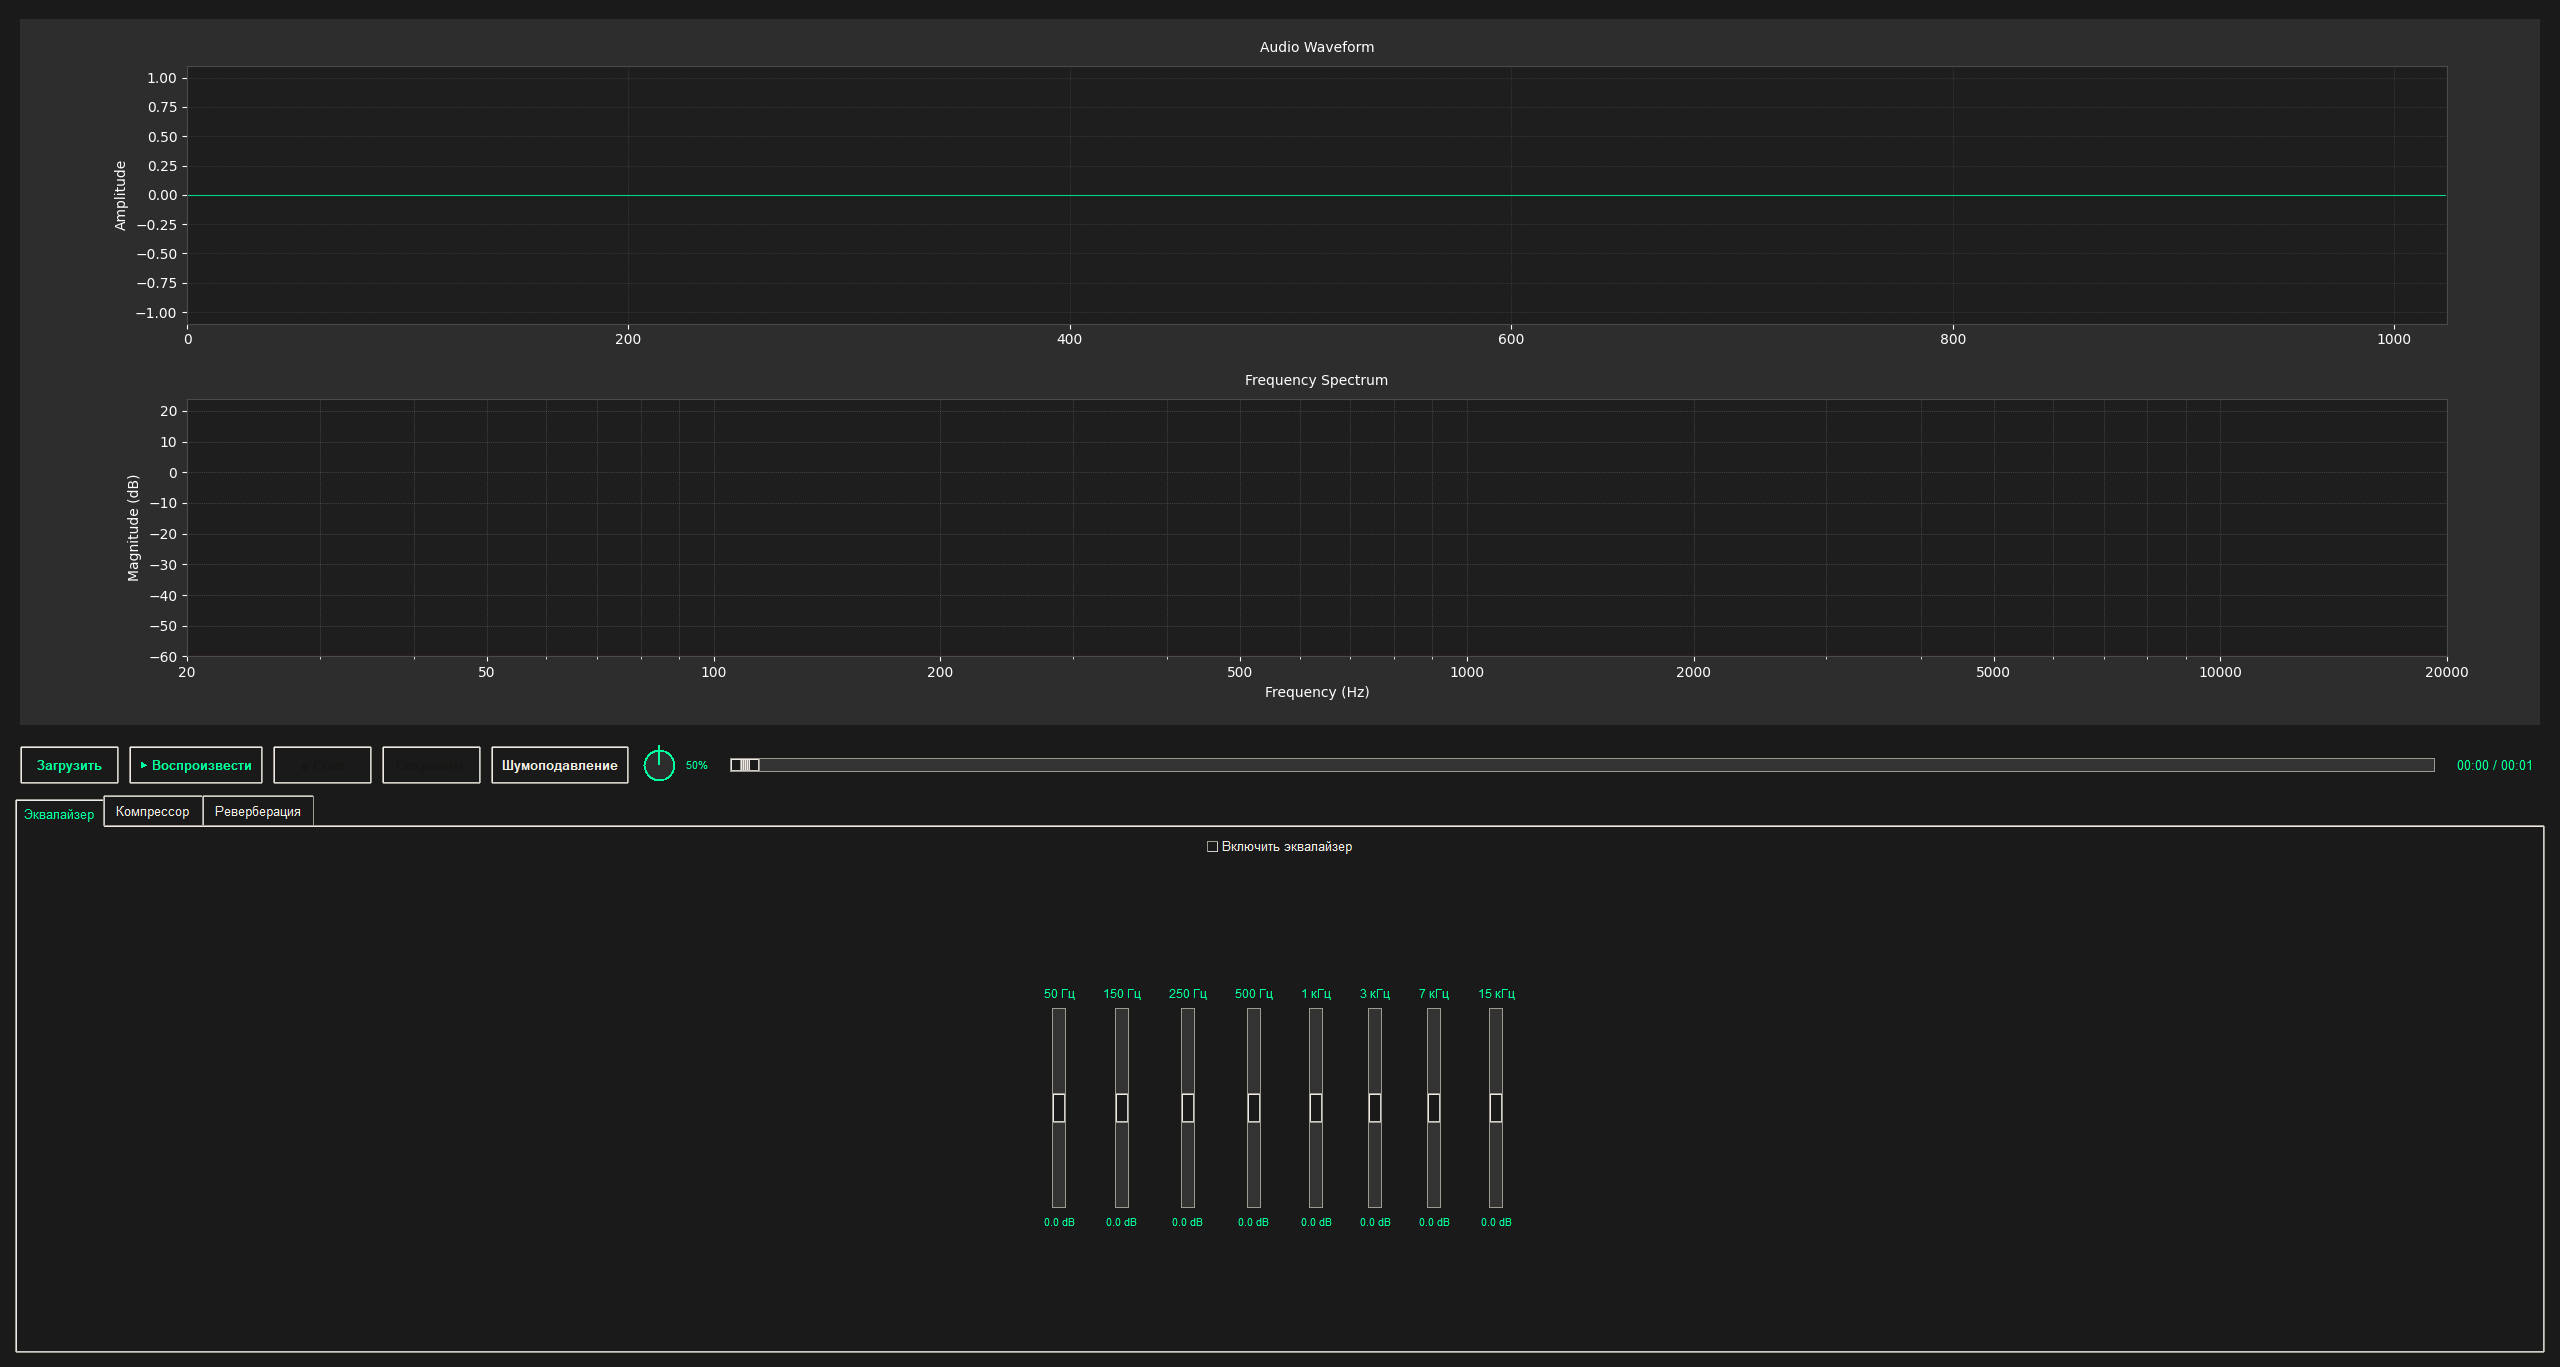
\includegraphics[width=0.8\linewidth]{Interface}}
	\caption{Интерфейс программы.}
	\label{Interface:image}
\end{figure}
\clearpage

\textbf{2) Загрузка аудиофайла}

Описание: Корректная загрузка аудиофайлов различных форматов (WAV, MP3, FLAC).

На рисунке \ref{LoadWindow:image} окно загрузки аудиофайла.

\begin{figure}[ht]
	\center{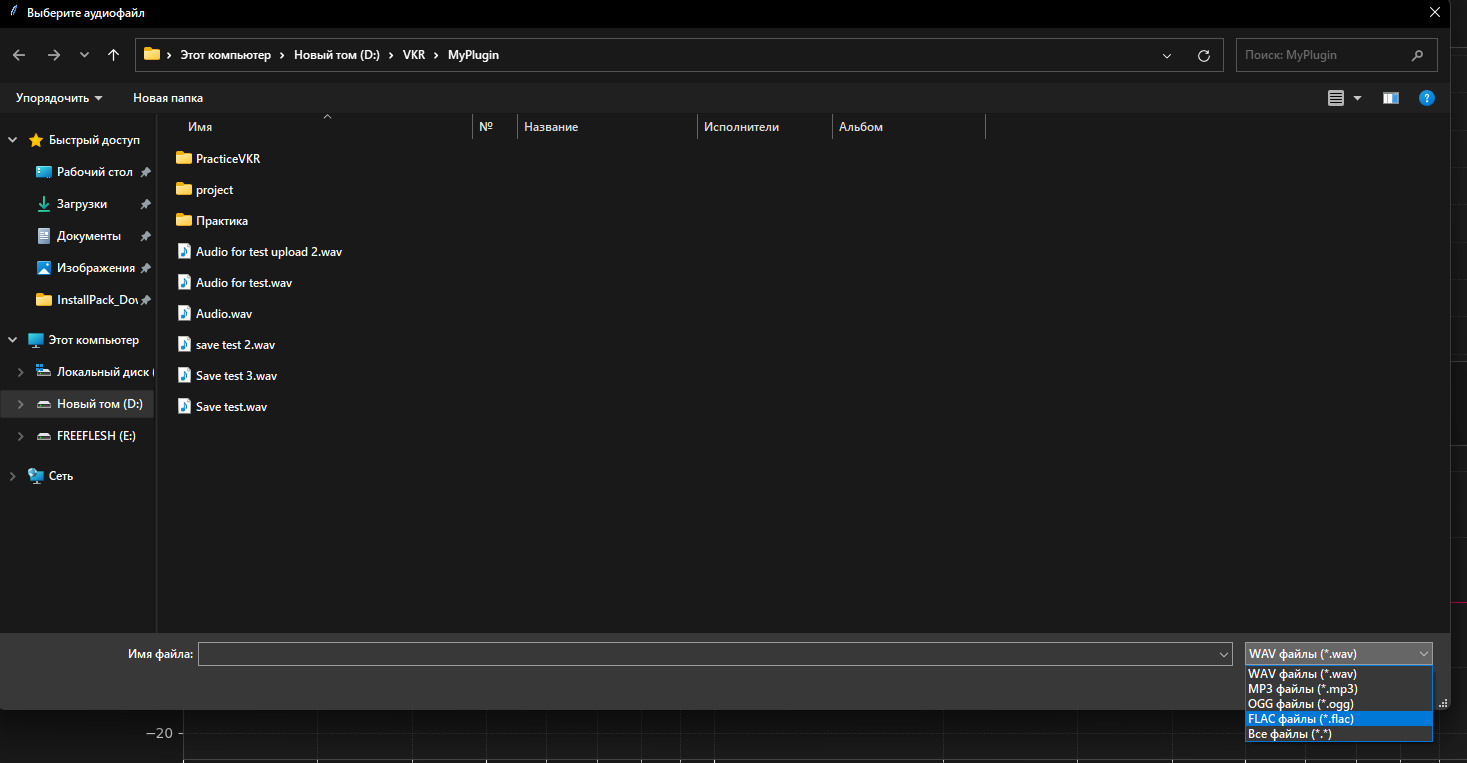
\includegraphics[width=0.8\linewidth]{LoadWindow}}
	\caption{Окно загрузки аудиофайла.}
	\label{LoadWindow:image}
\end{figure}

На рисунке \ref{InterLoad:image} интерфейс программы при успешной загрузки аудиофайла.

\begin{figure}[ht]
	\center{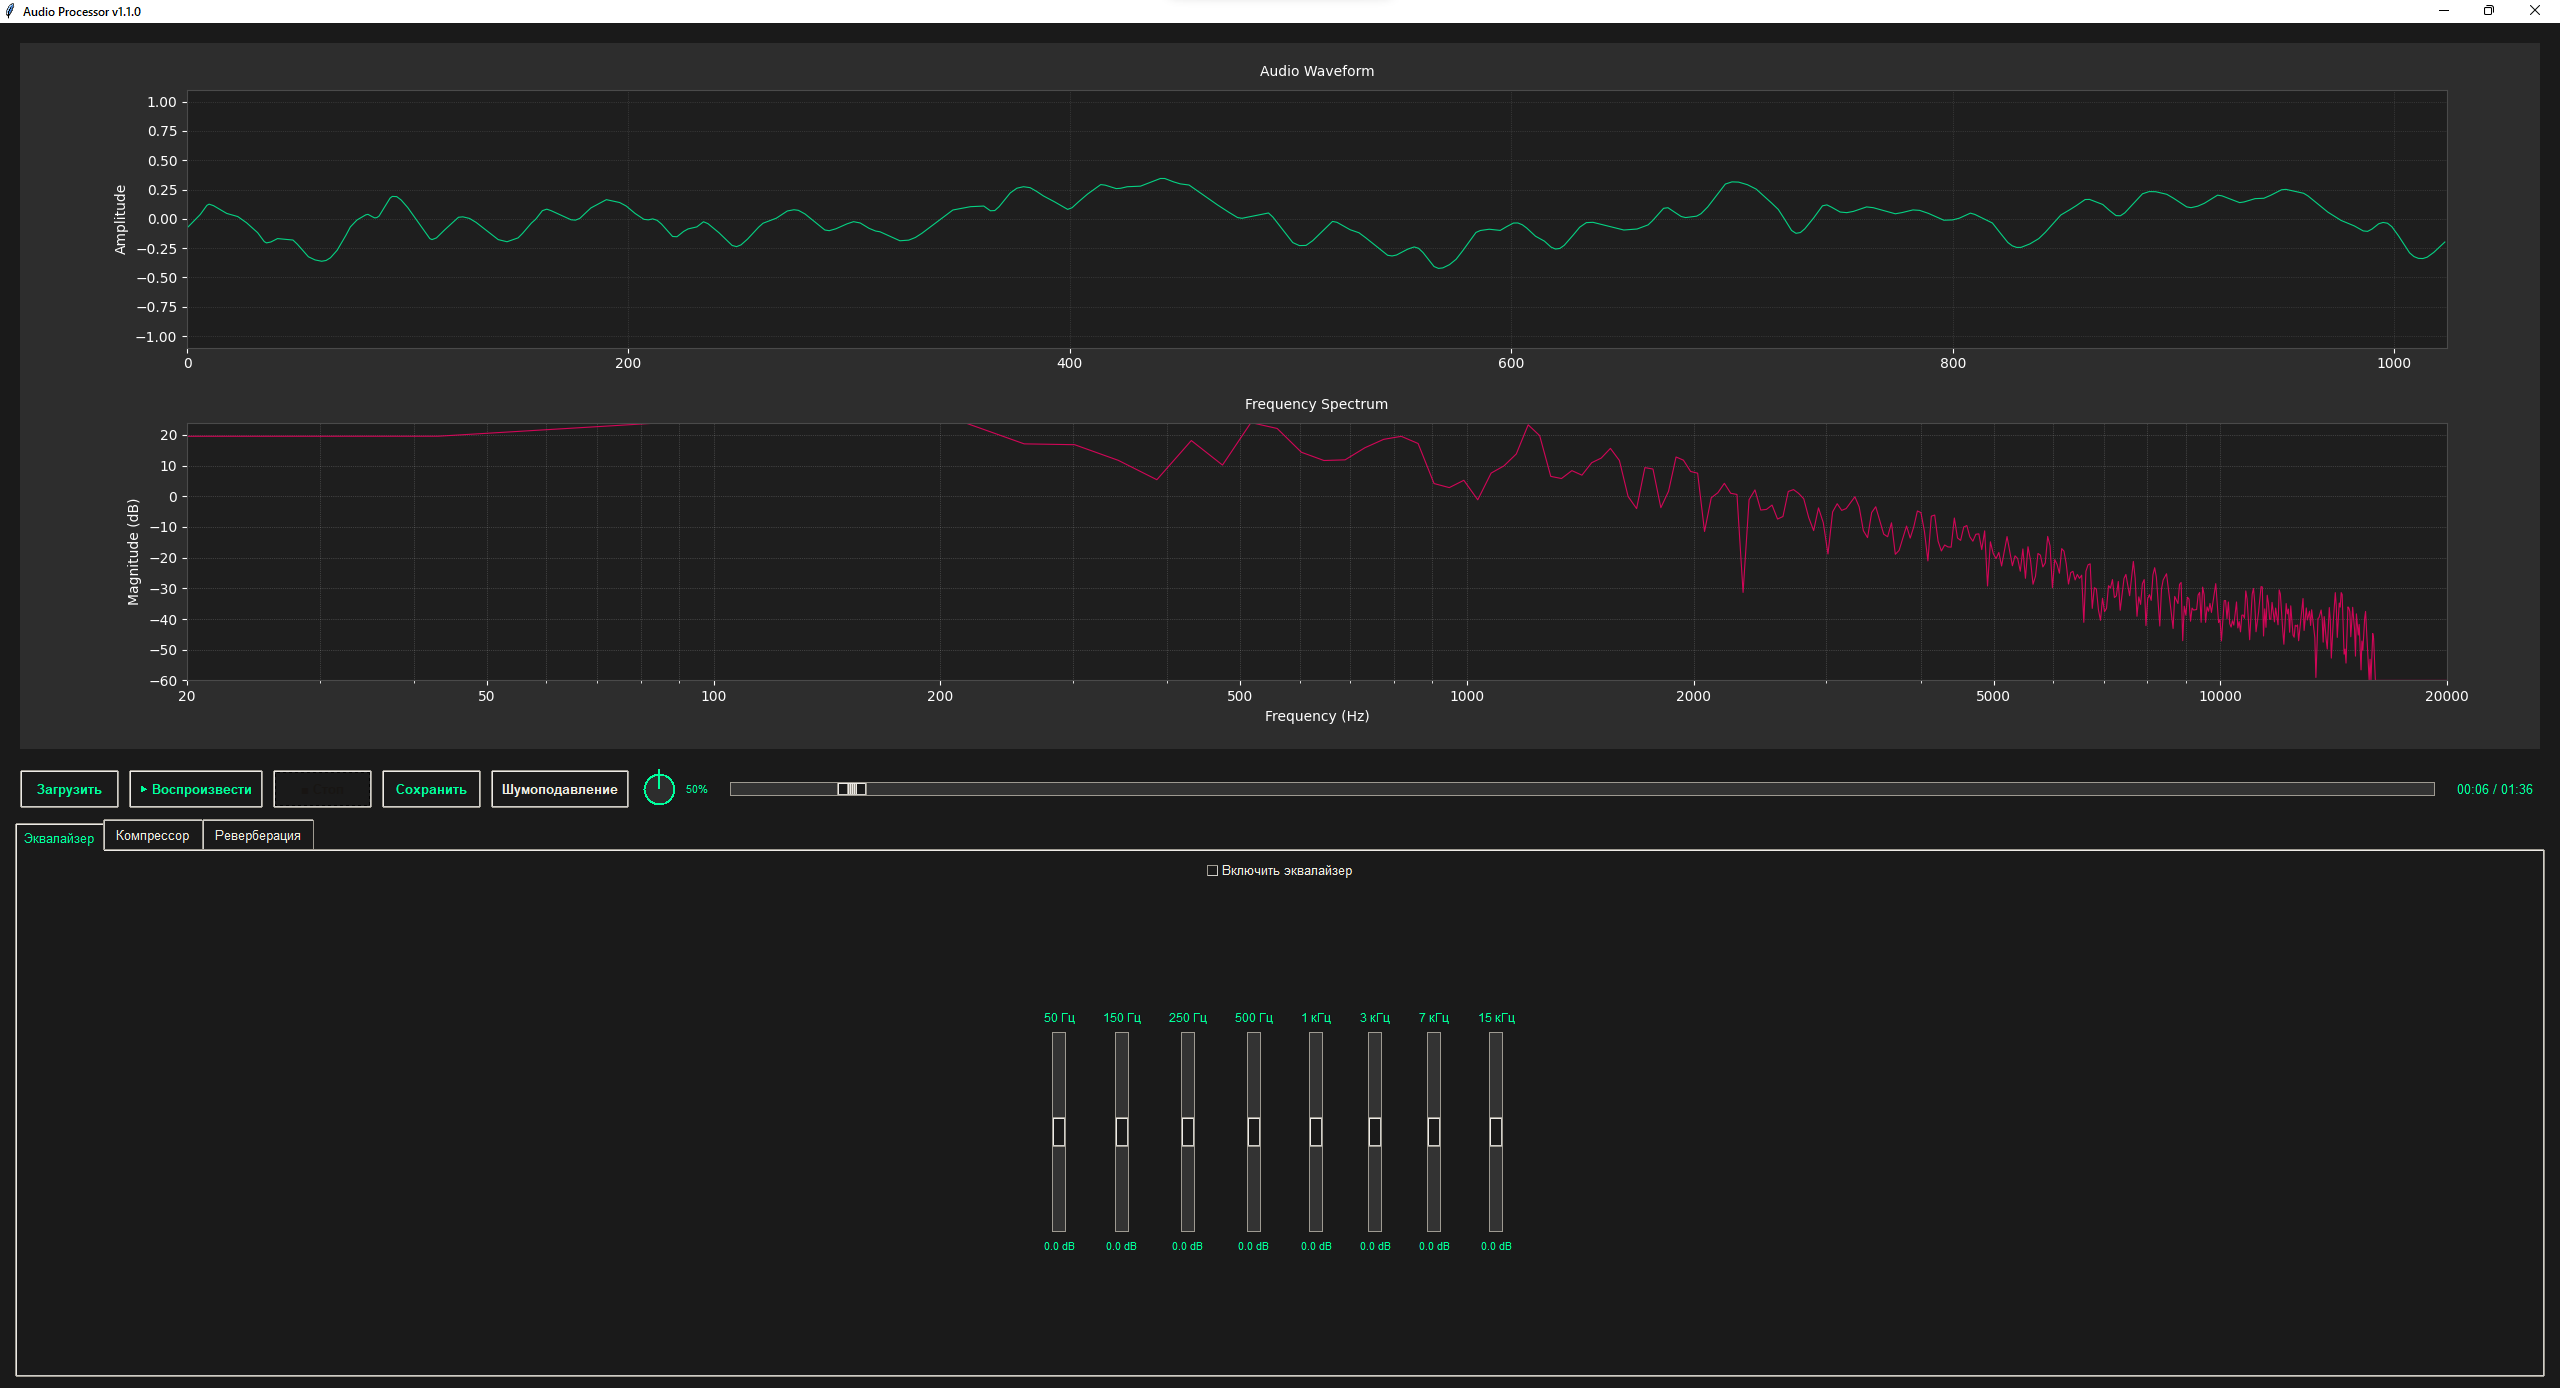
\includegraphics[width=0.8\linewidth]{InterLoad}}
	\caption{Интерфейс программы при успешной загрузки аудиофайла.}
	\label{InterLoad:image}
\end{figure}
\clearpage

\textbf{3) Корректное воспроизведение и остановка аудио}

Описание: При восопроизведении и остановки проигрывания аудио, соответственно, воспроизводится и останавливается. Так же перемещается ползунок метки воспроизведения в соответствии времени воспроизведения и при перемещени пользователем, аудио воспроизводится с момента, на который переместил пользователь.

На рисунке \ref{SliderTime:image} перемещение ползунка при воспроизведении.

\begin{figure}[ht]
	\center{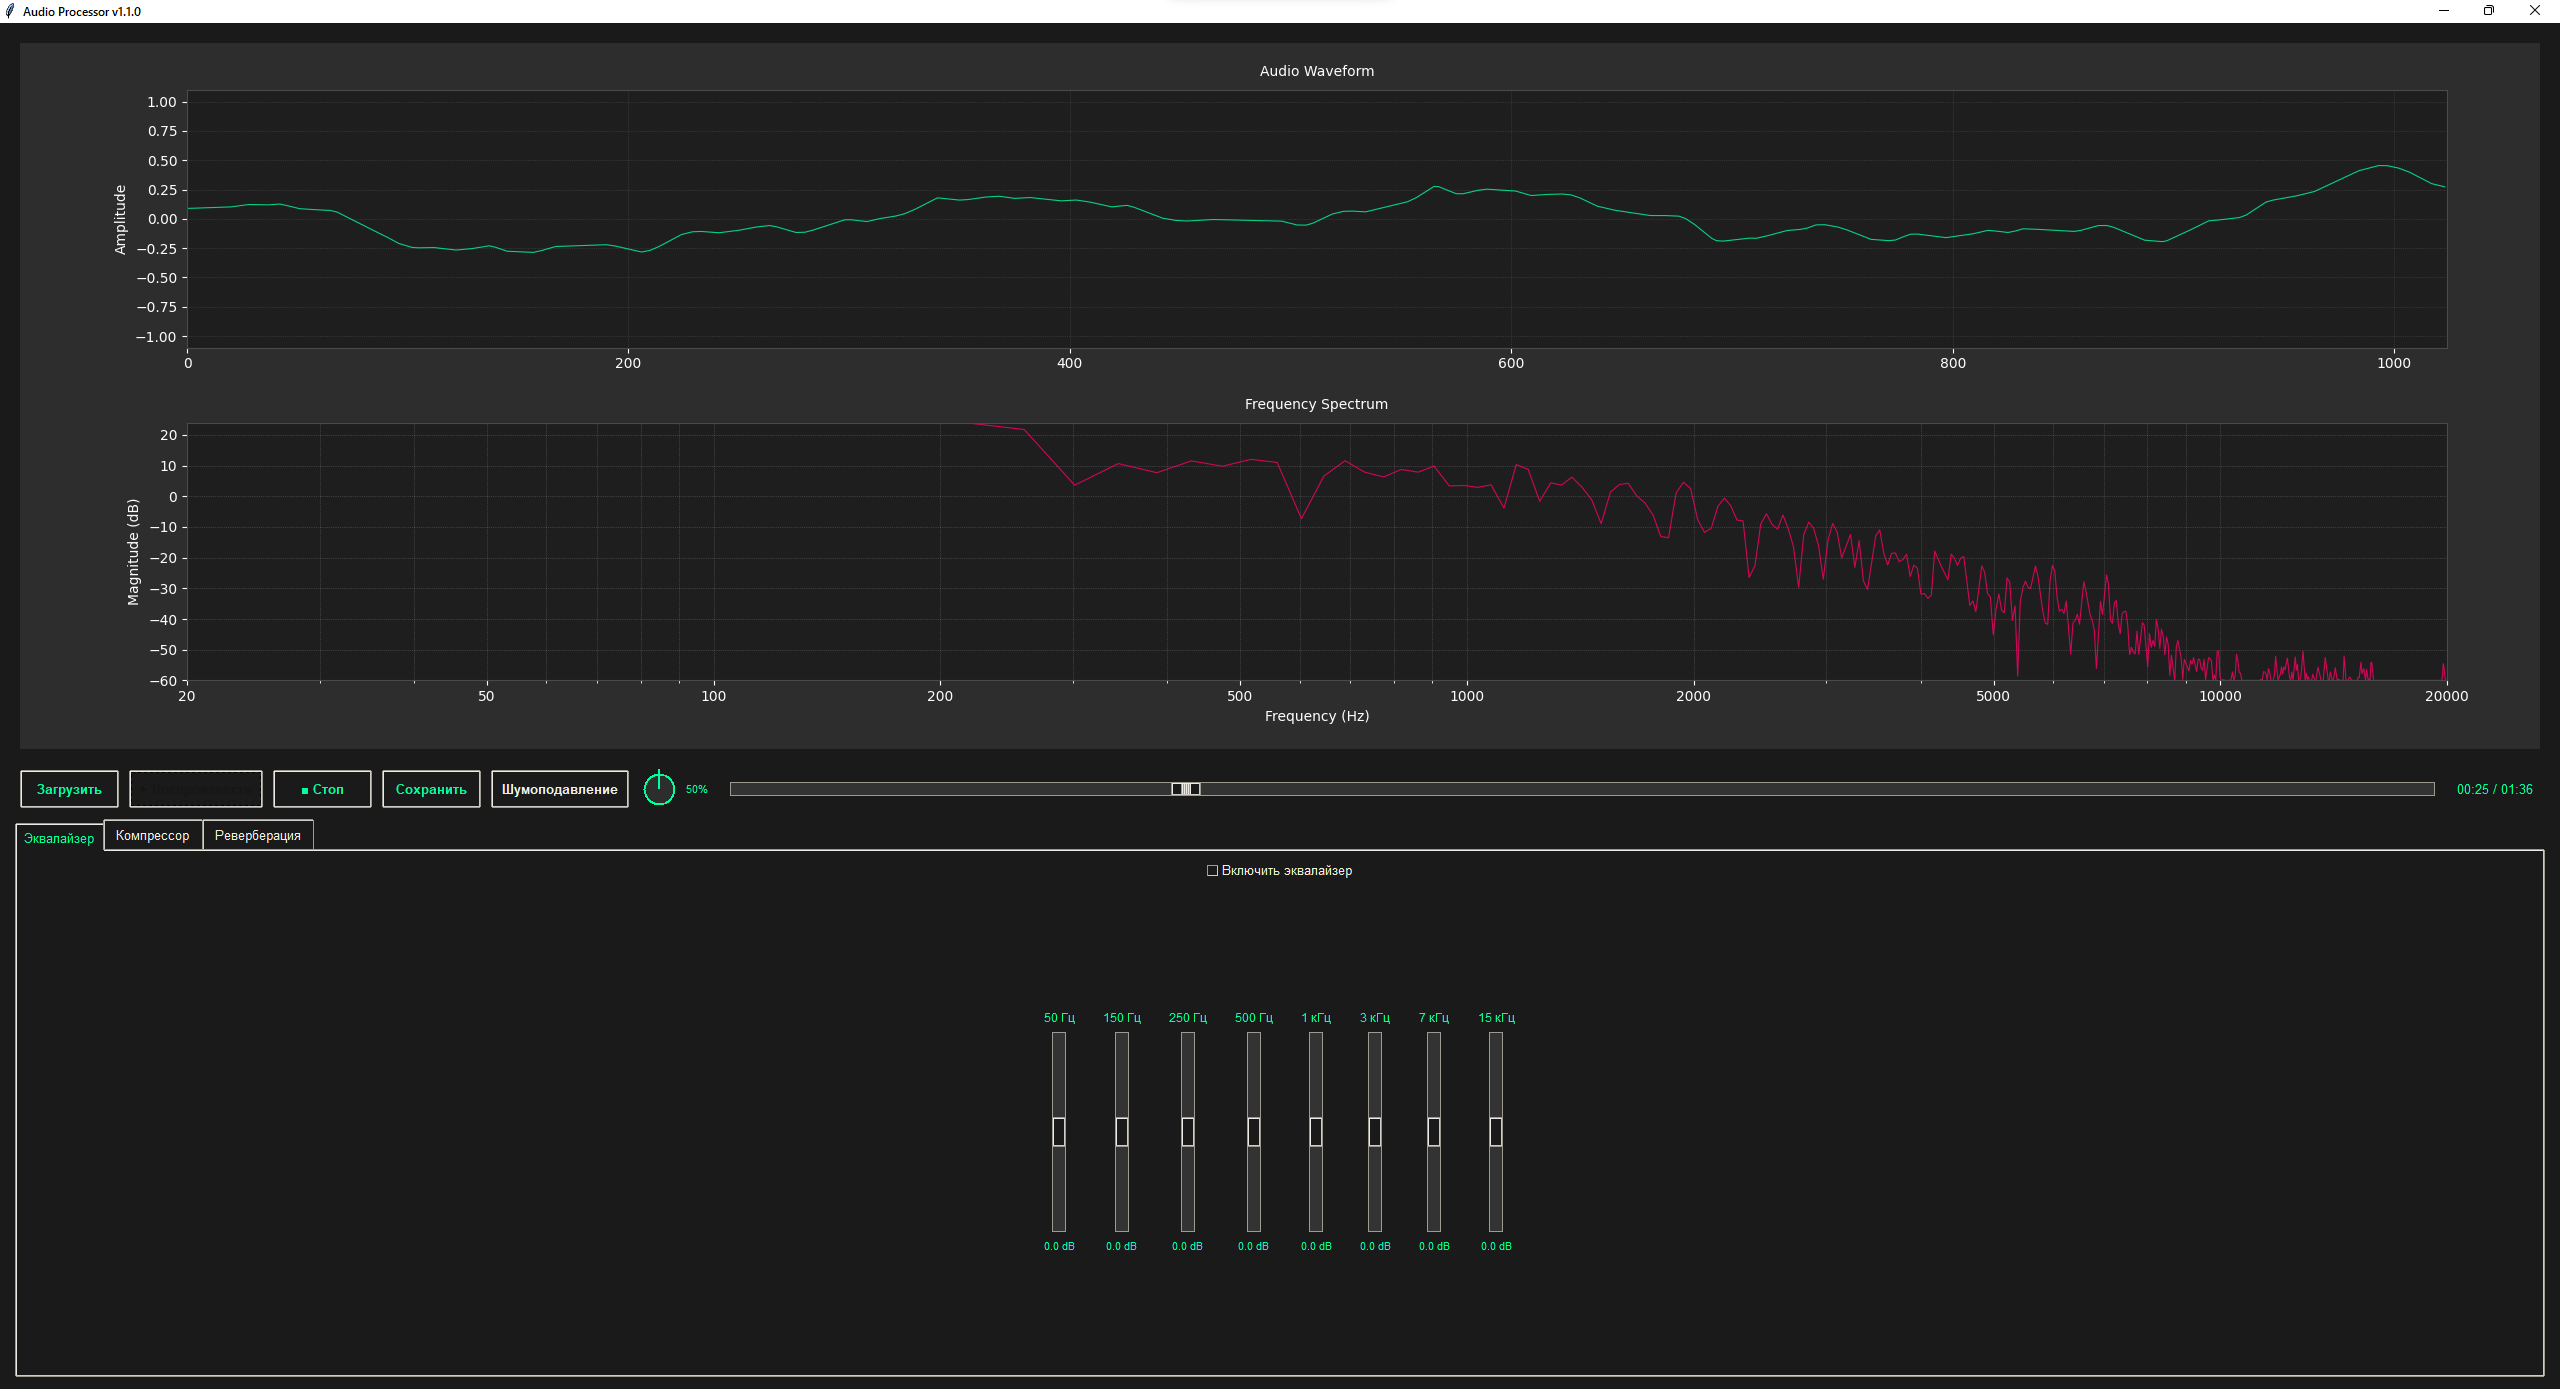
\includegraphics[width=0.7\linewidth]{SliderTime}}
	\caption{Интерфейс программы при перемещении ползунка управления воспроизведением.}
	\label{SliderTime:image}
\end{figure}

На рисунке \ref{Stop:image} остановка воспроизведения аудио.

\begin{figure}[ht]
	\center{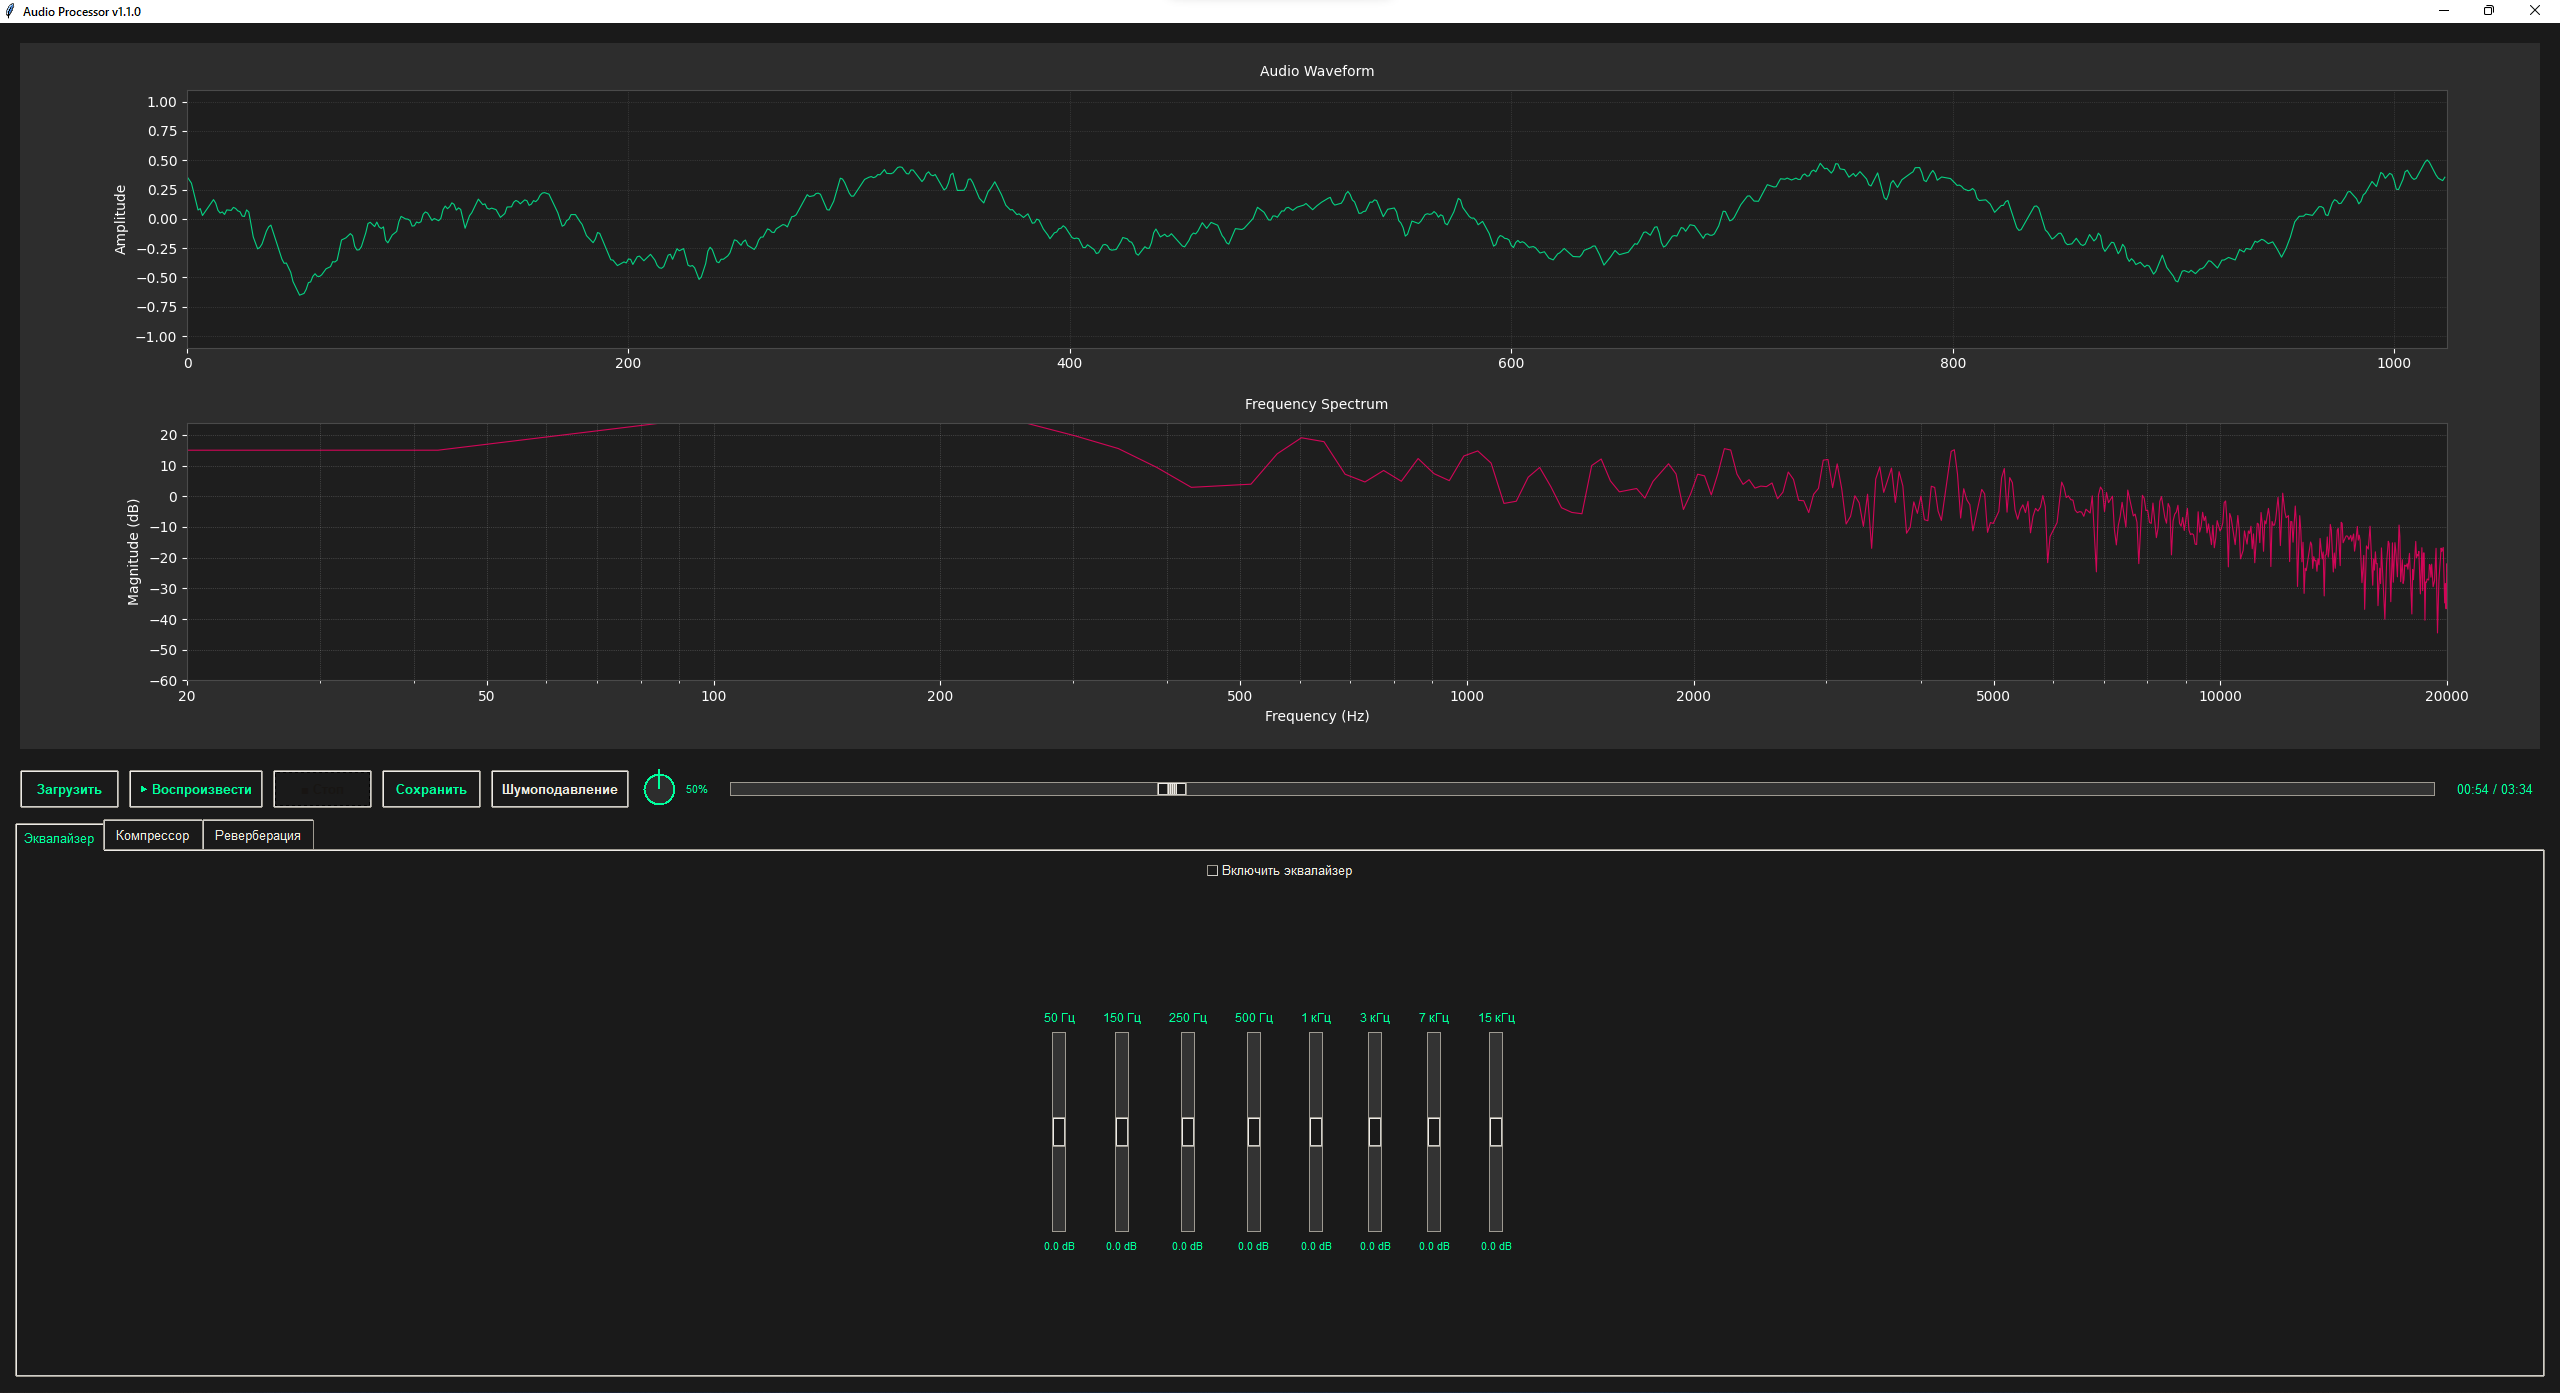
\includegraphics[width=0.7\linewidth]{Stop}}
	\caption{Интерфейс программы при остановки воспроизведения аудио.}
	\label{Stop:image}
\end{figure}
\clearpage

\textbf{4) Обработка аудиосигнала в реальном времени}

Описание: При восопроизведении аудиофайла графики формы волны и АЧХ отображают данные аудио в реальном времени.

На рисунке \ref{Graph:image} отображение графиков формы волны и АЧХ в реальном времени.

\begin{figure}[ht]
	\center{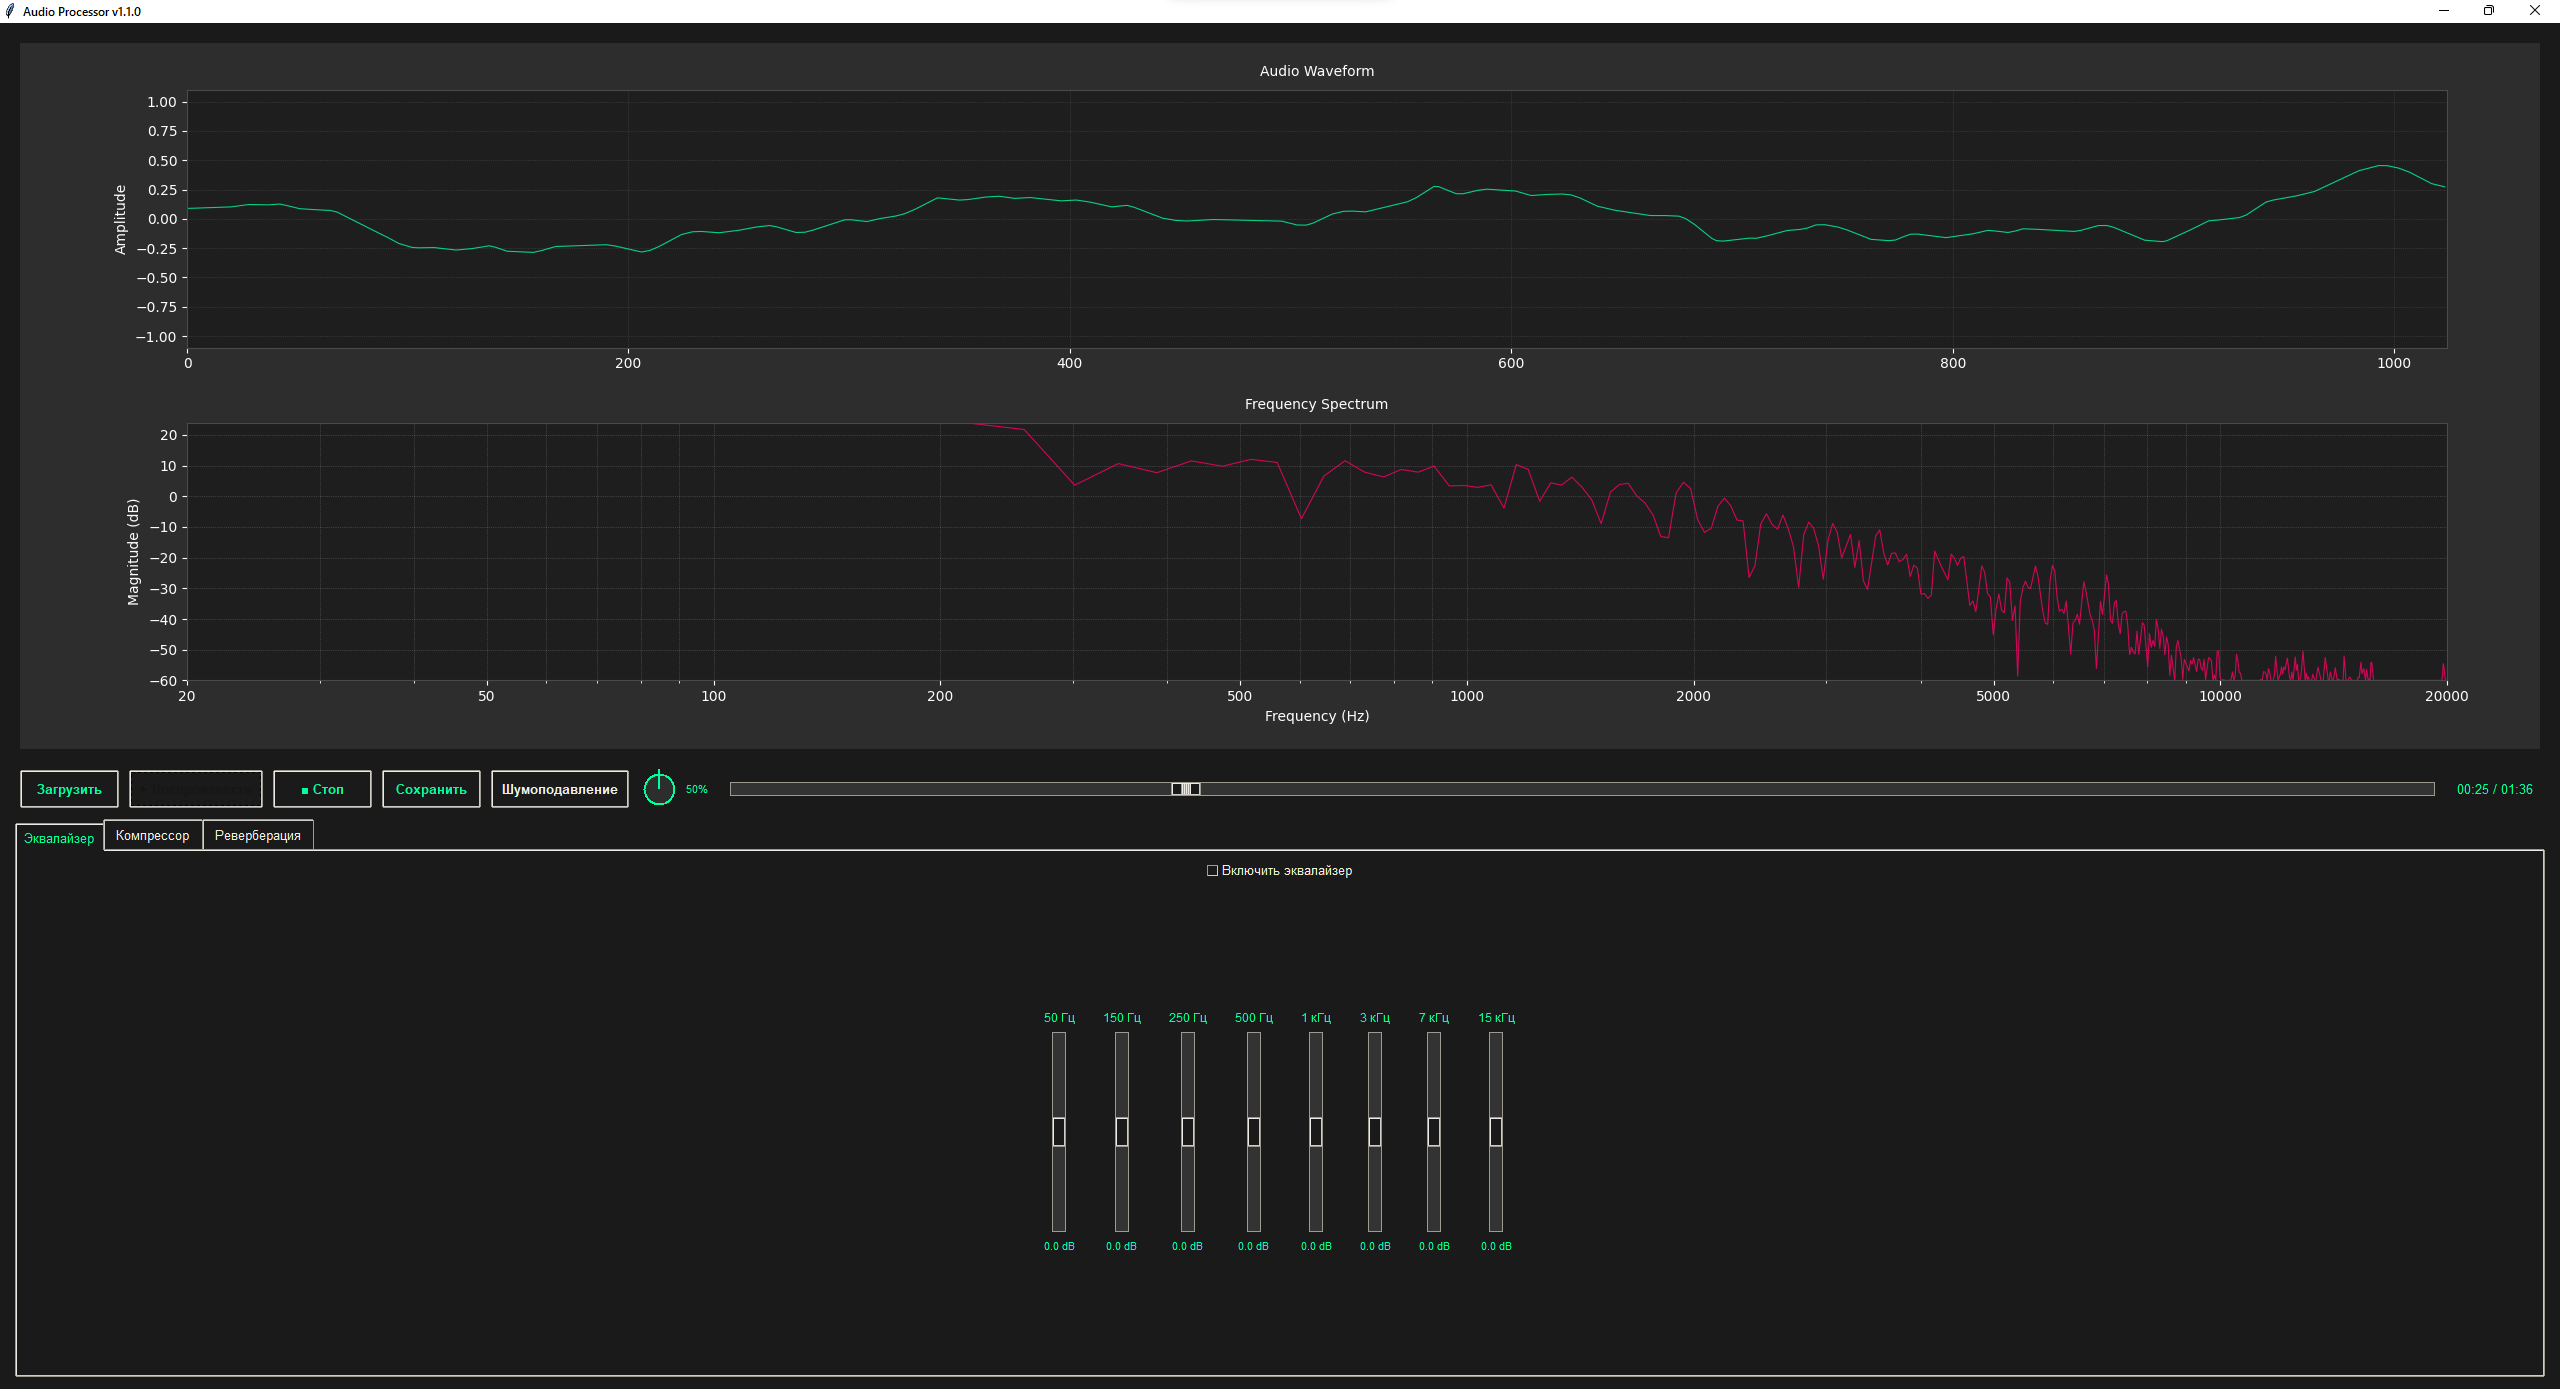
\includegraphics[width=0.8\linewidth]{Graph}}
	\caption{Отображение графиков.}
	\label{Graph:image}
\end{figure}

На рисунке \ref{GraphSilence:image} отображение графиков формы волны и АЧХ при тишине в аудиофайле.

\begin{figure}[ht]
	\center{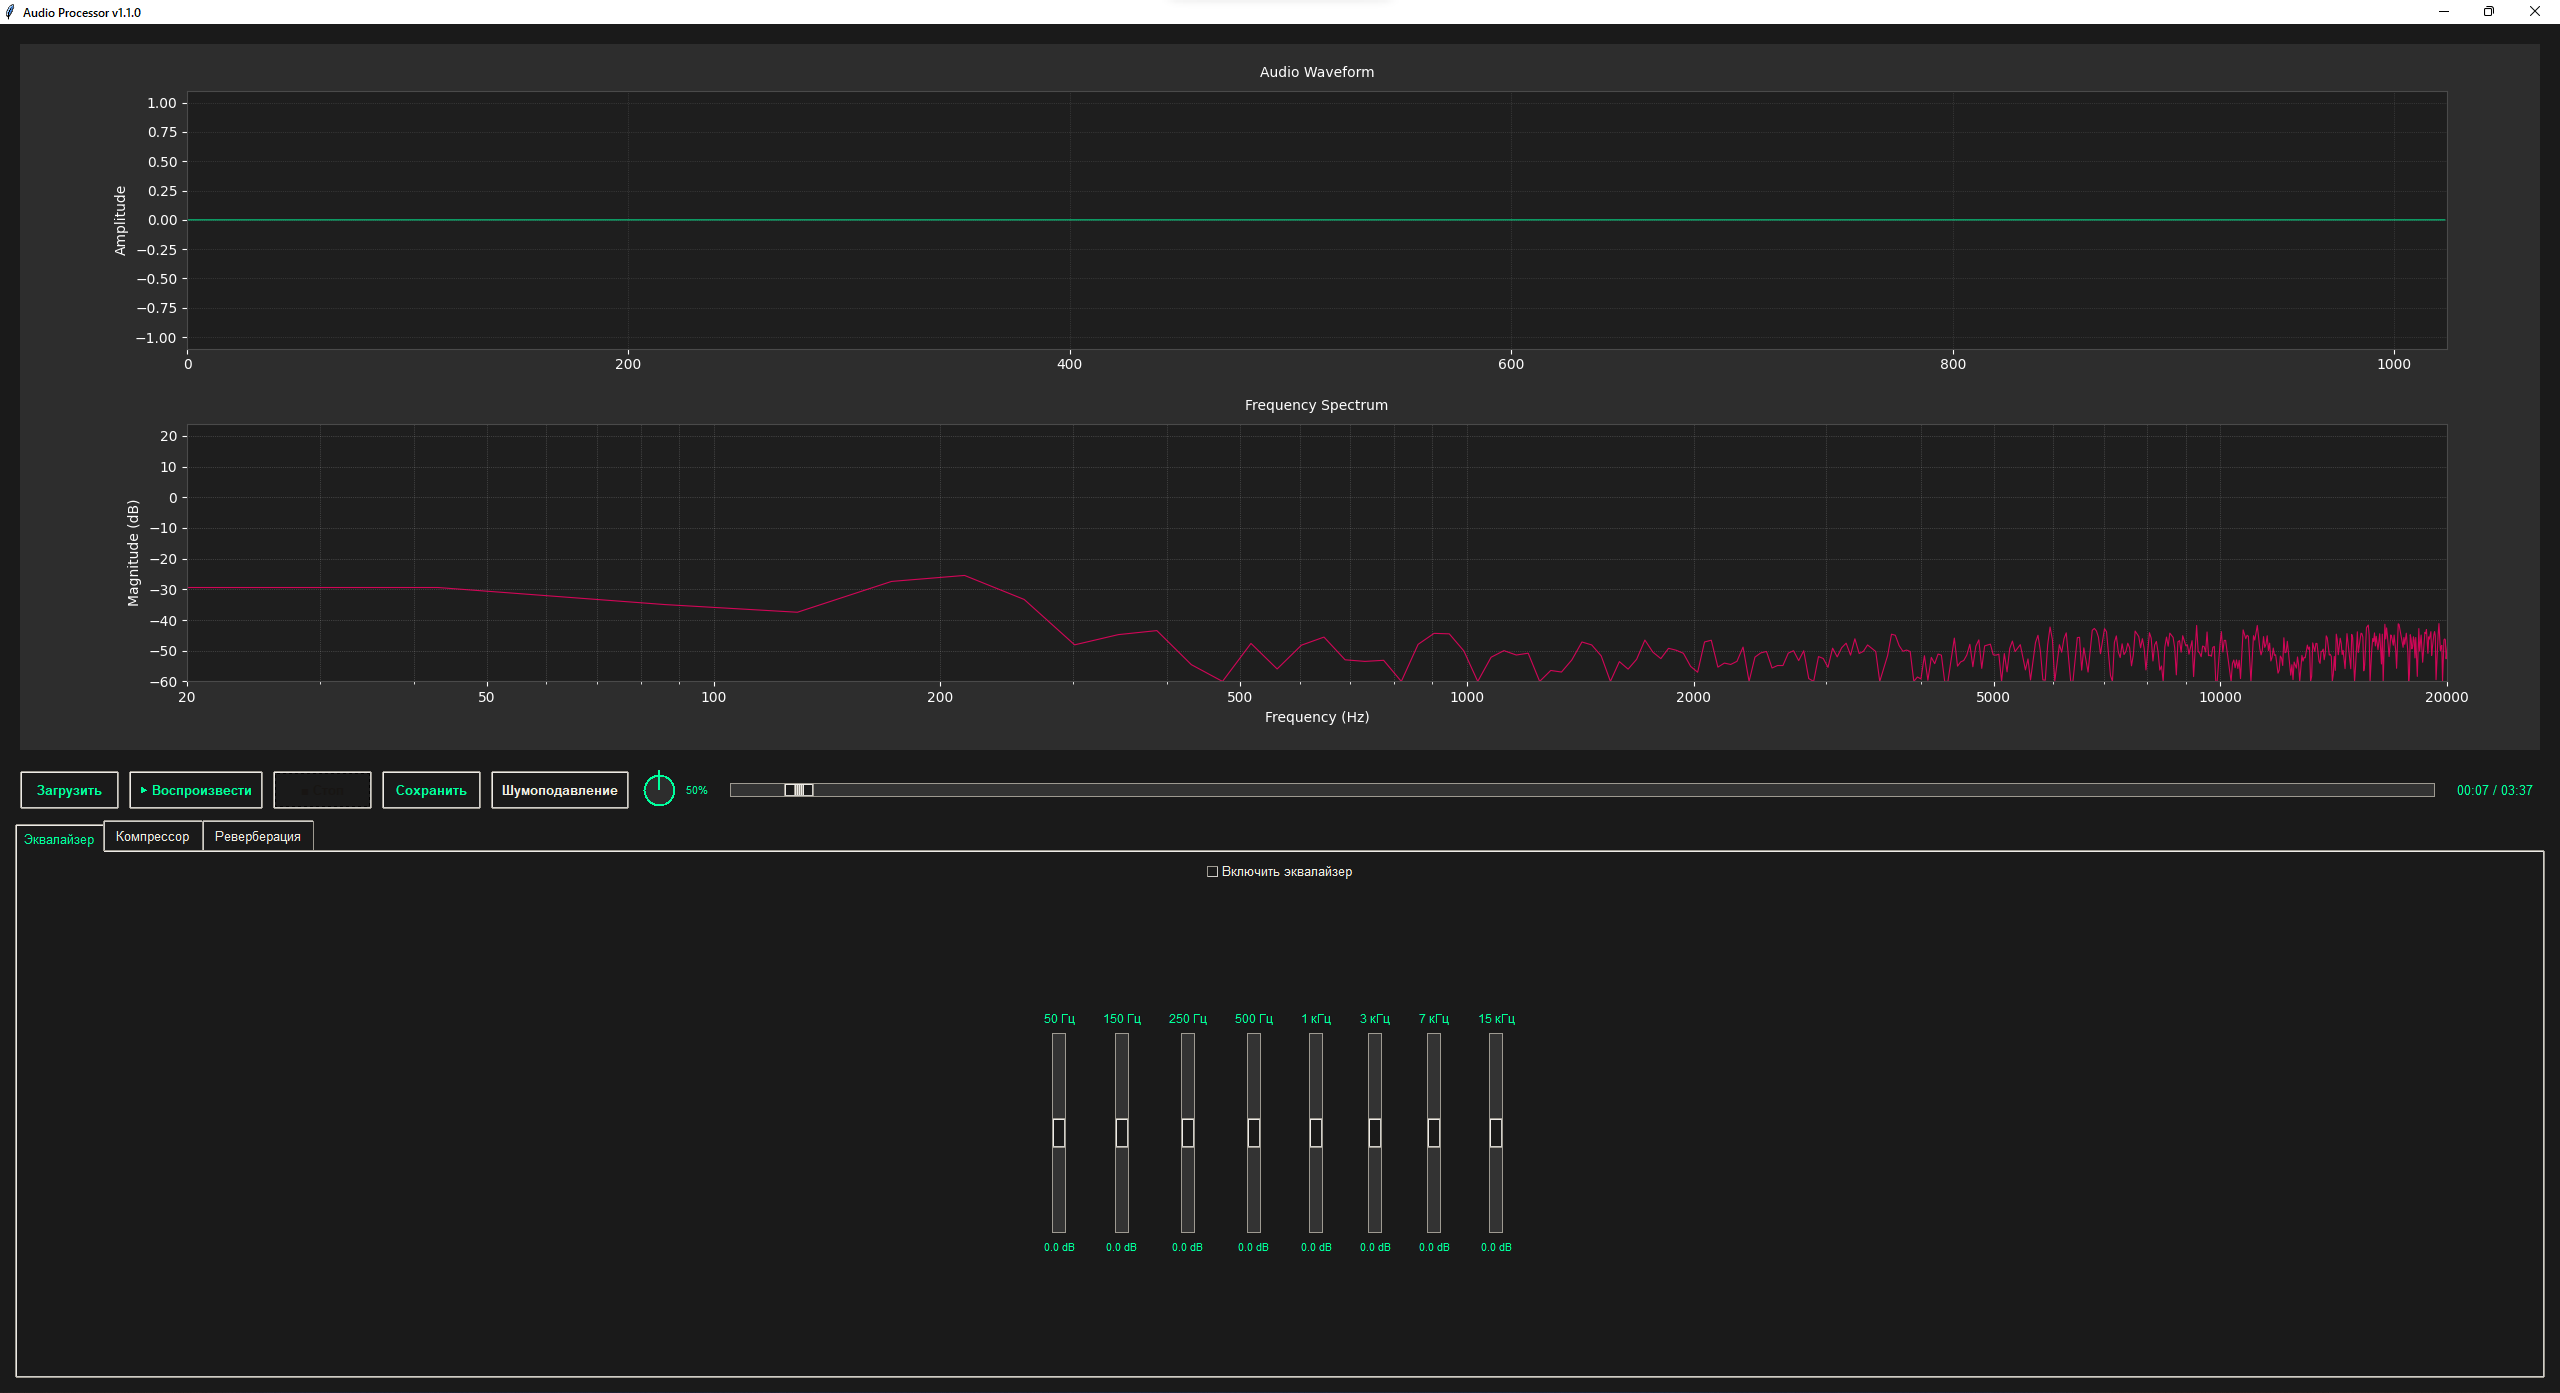
\includegraphics[width=0.8\linewidth]{GraphSilence}}
	\caption{Отображение графиков при тишине в аудиофайле.}
	\label{GraphSilence:image}
\end{figure}
\clearpage

\textbf{5) Изменение параметров эквалайзера}

Описание: При изменении параметров эквалайзера, регулировки ползунков, все изменения применяются сразу, без задержек и прерываний. Так же изменяются графики формы волны и АЧХ.

На рисунке \ref{EQParam:image} изменение параметров эквалайзера.

\begin{figure}[ht]
	\center{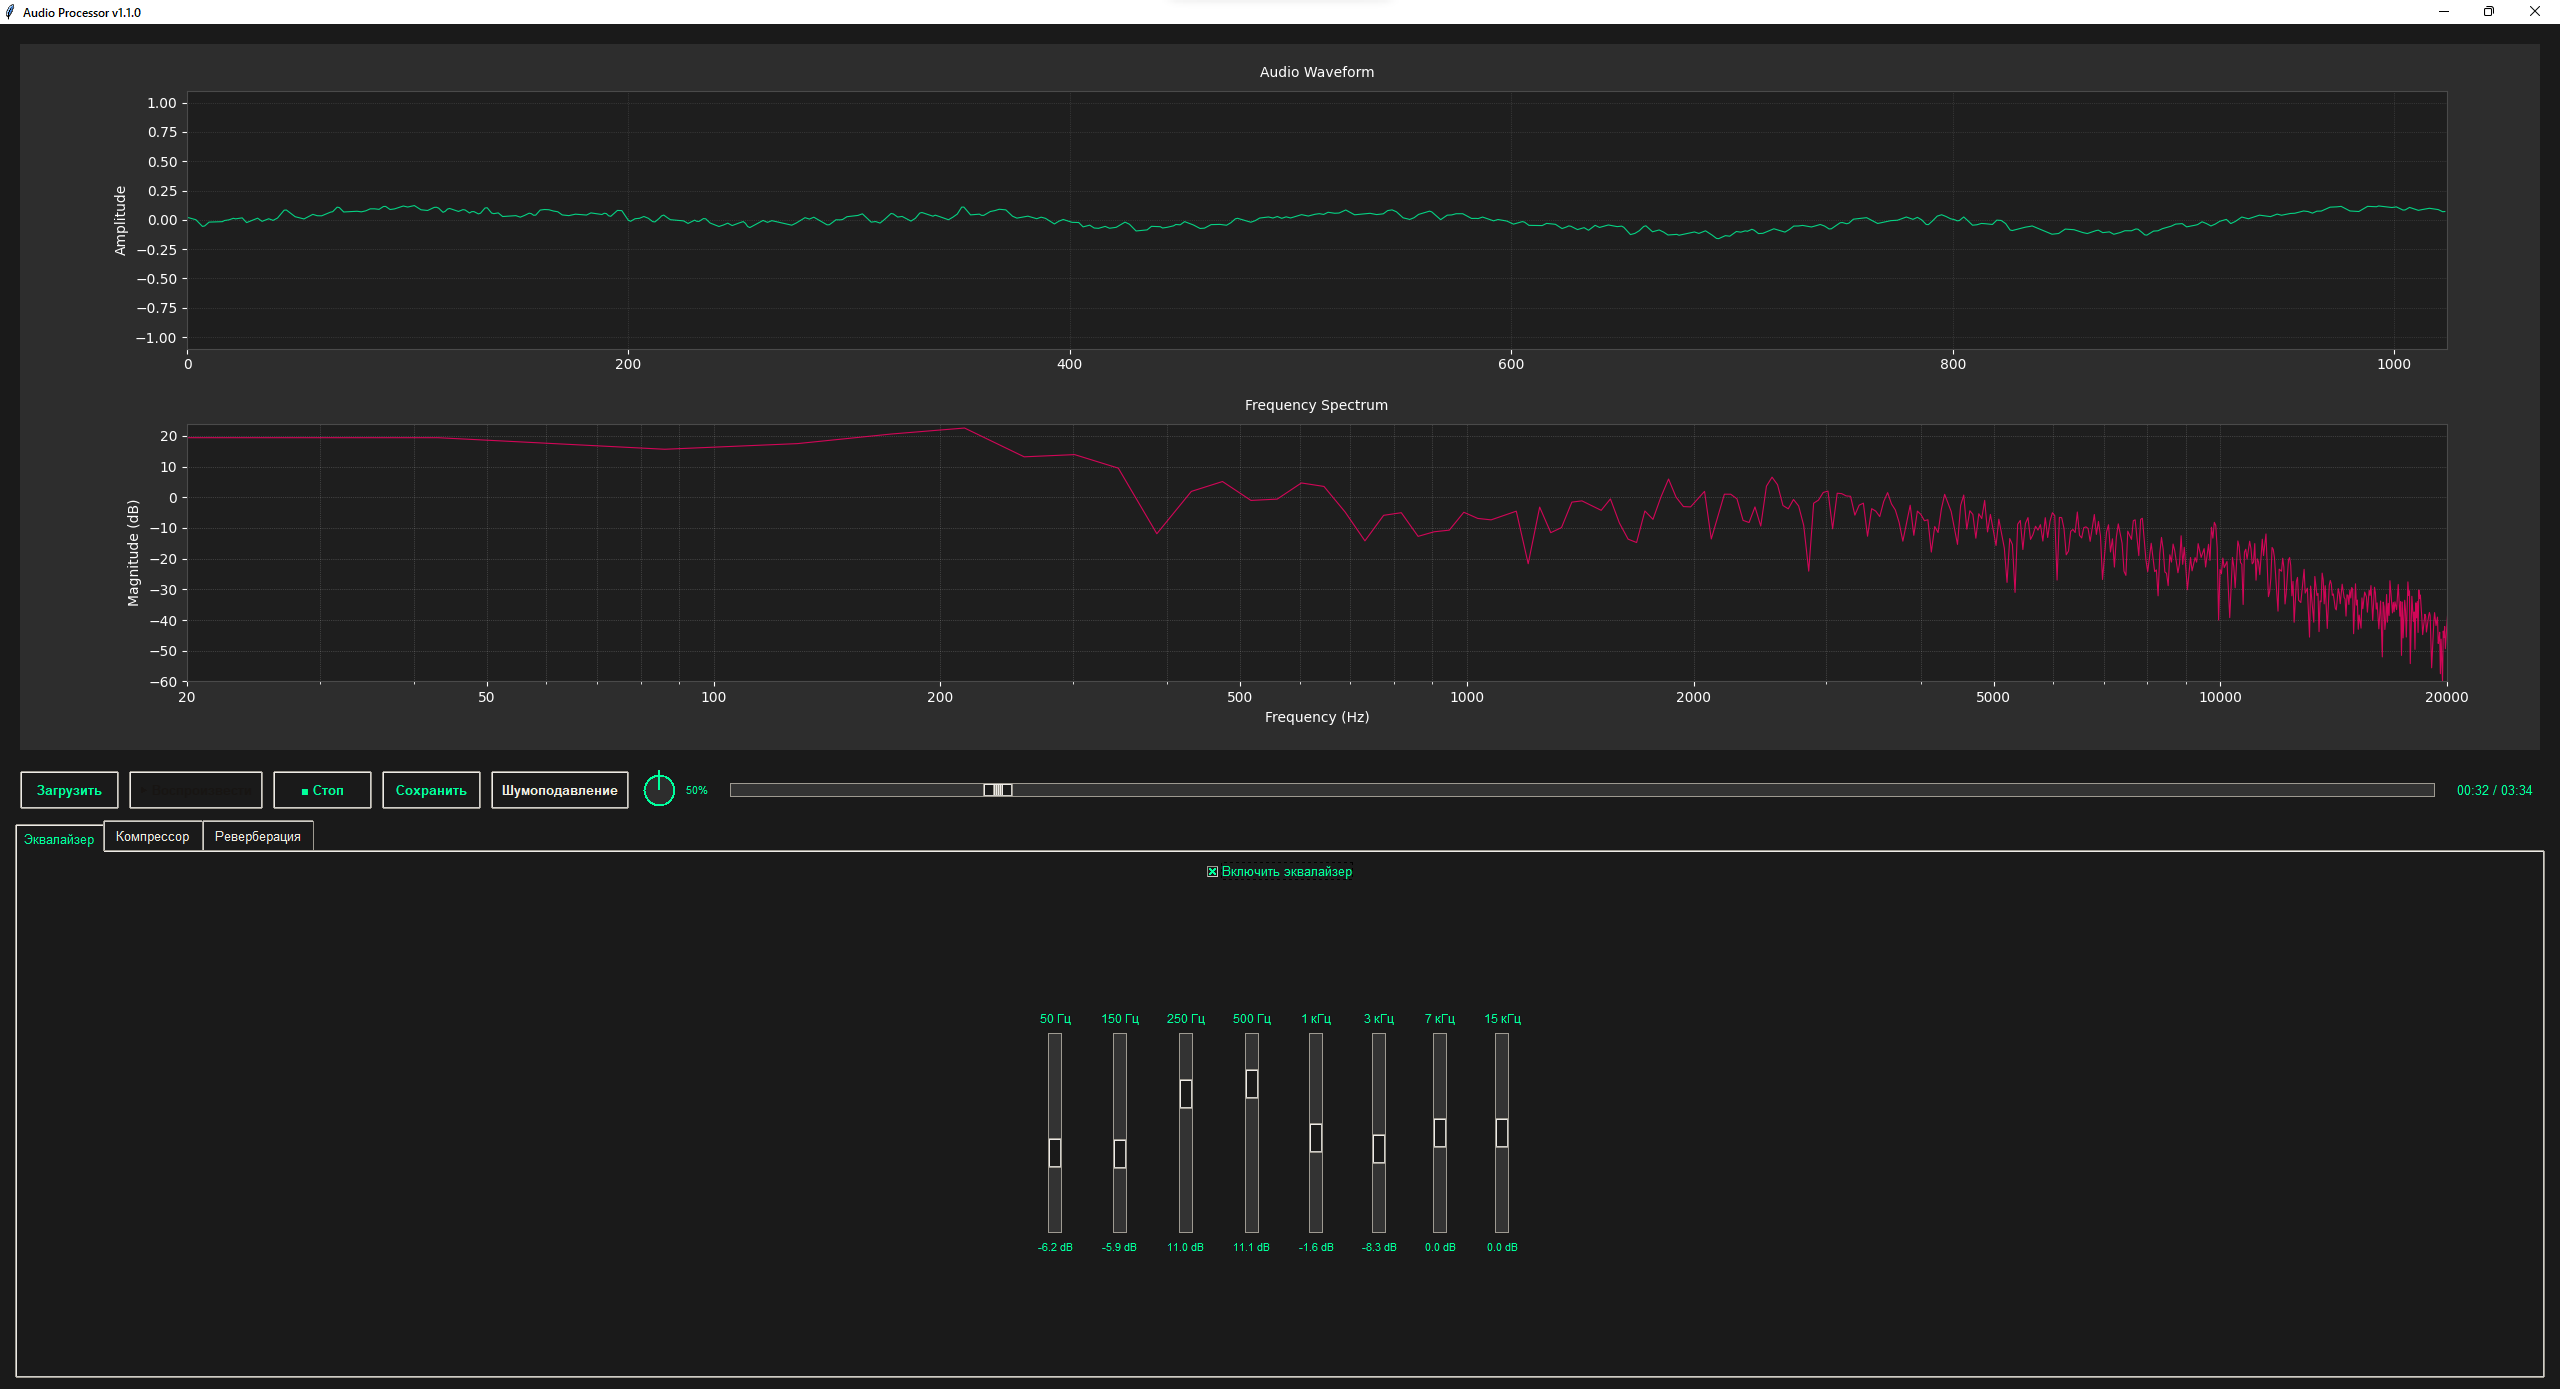
\includegraphics[width=0.8\linewidth]{EQParam}}
	\caption{Изменение параметров эквалайзера.}
	\label{EQParam:image}
\end{figure}

На рисунке \ref{EQParamOff:image} отображение графиков при выключенном эквалайзере.

\begin{figure}[ht]
	\center{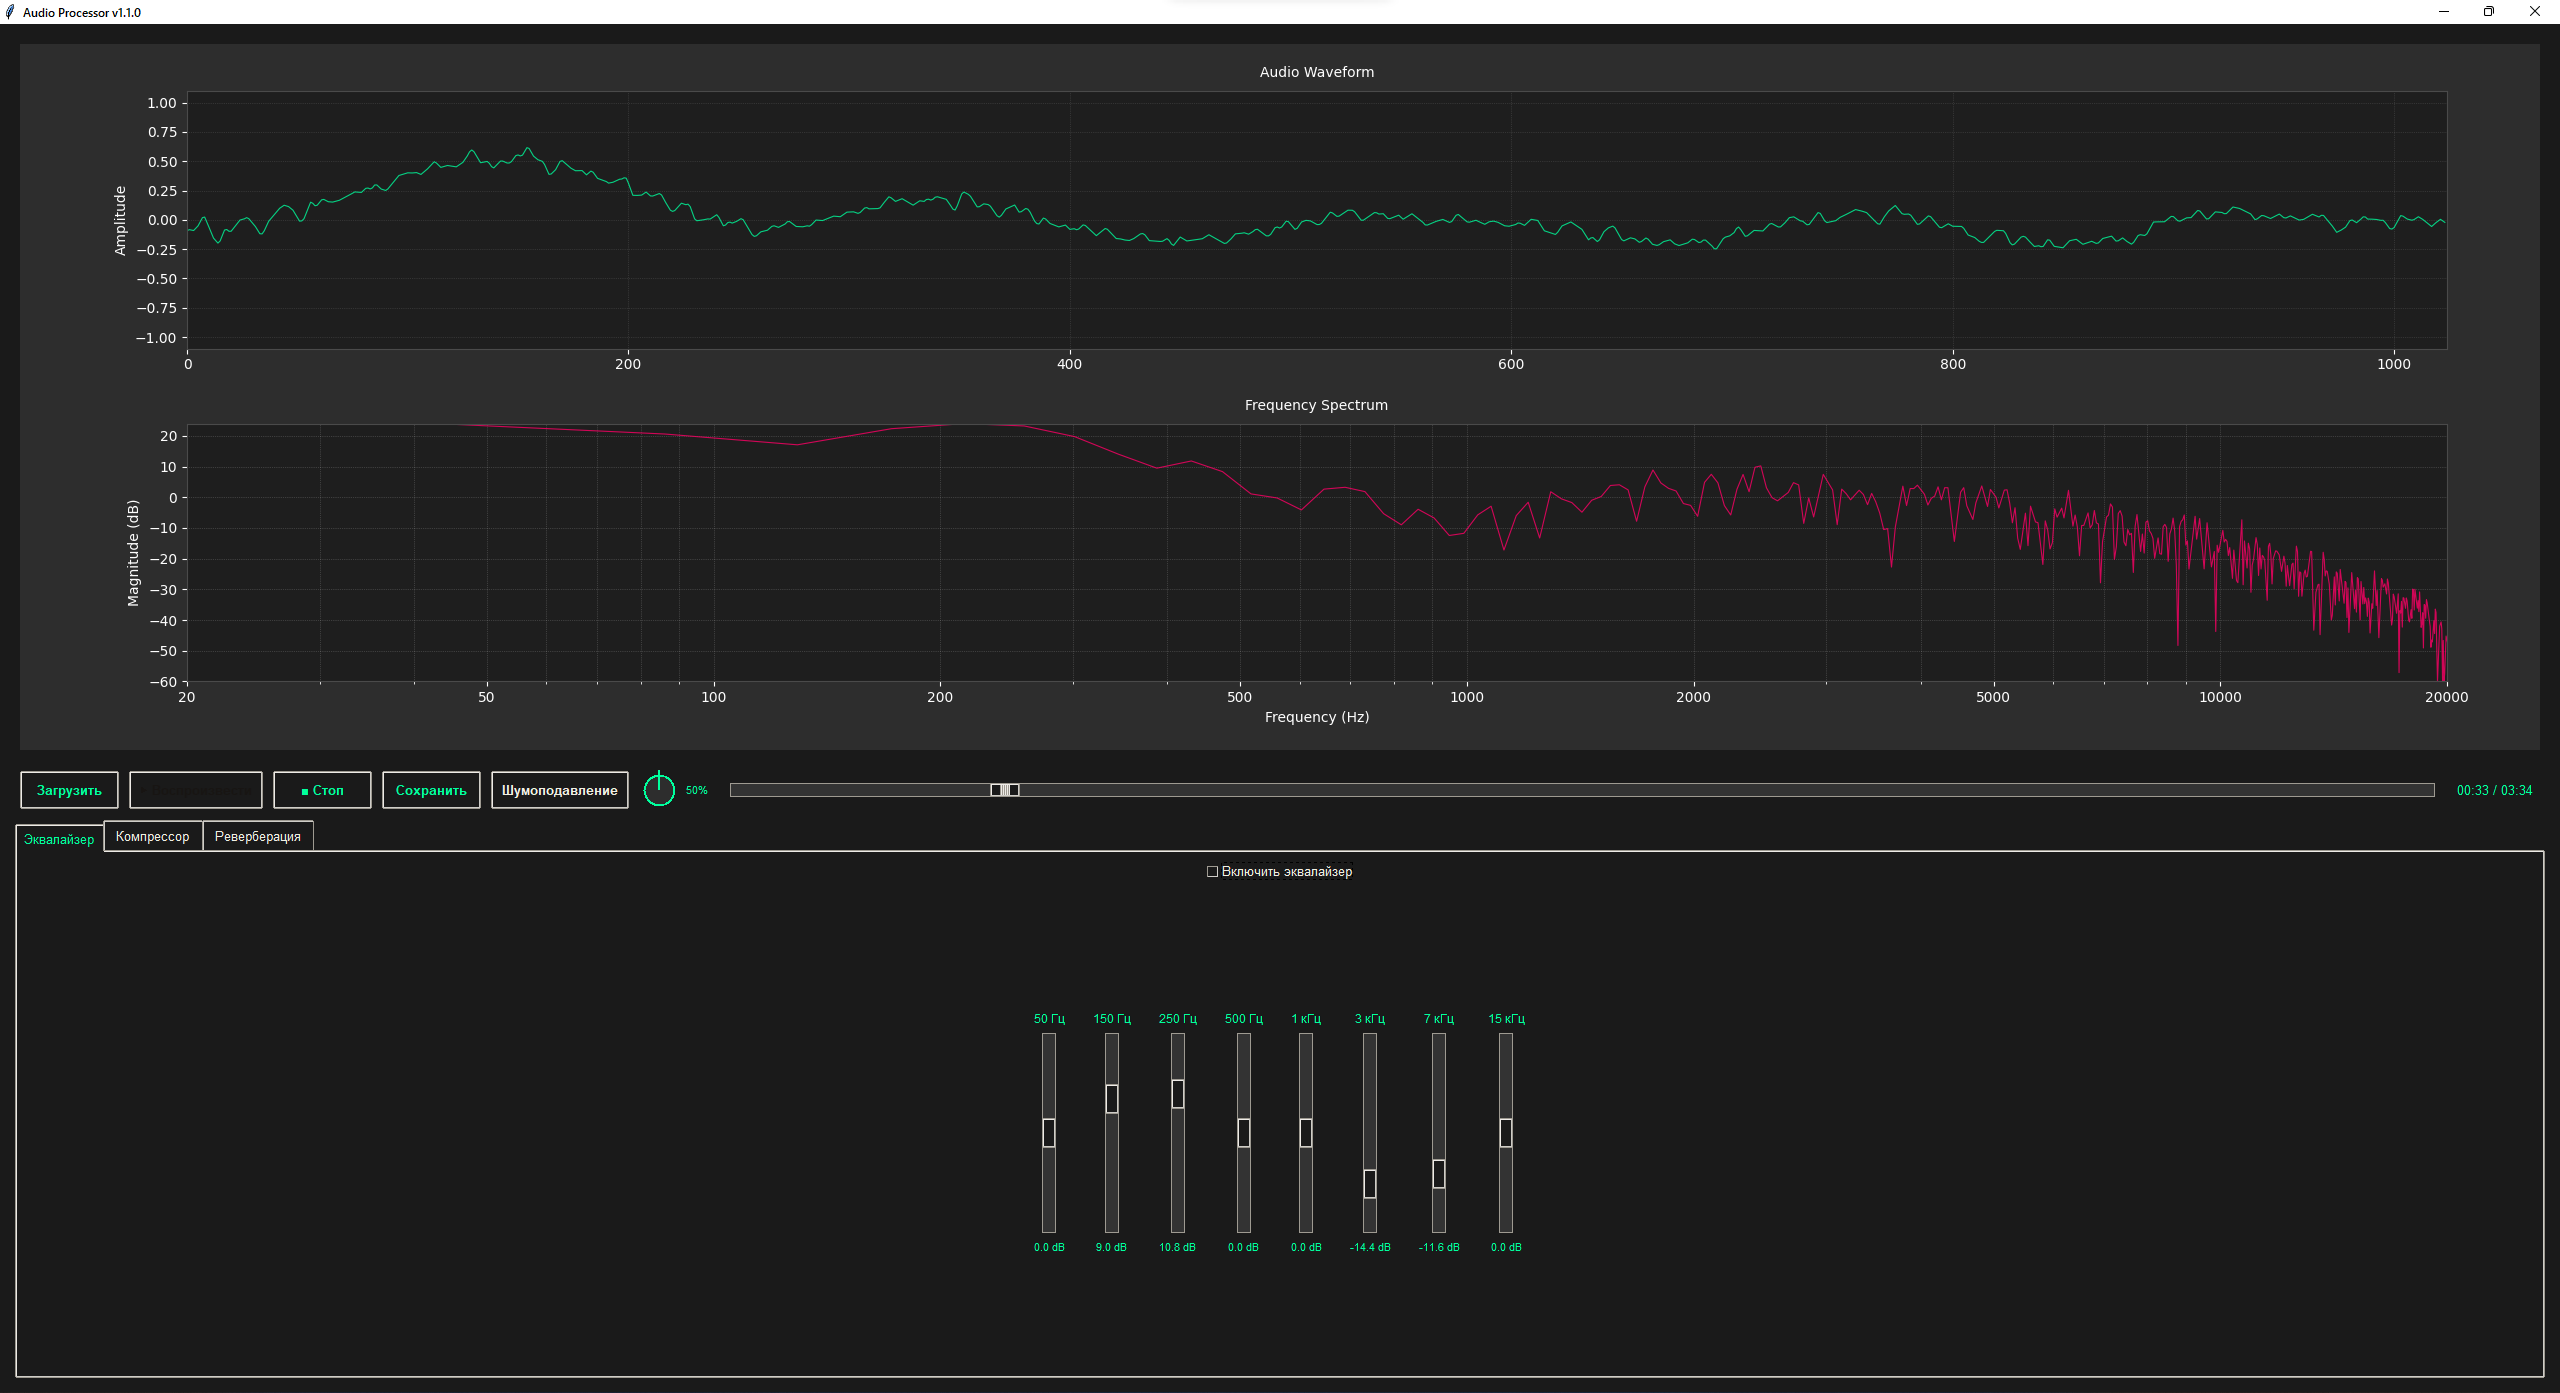
\includegraphics[width=0.8\linewidth]{EQParamOff}}
	\caption{Отображение графиков при выключенном эквалайзере.}
	\label{EQParamOff:image}
\end{figure}
\clearpage

\textbf{6) Изменение параметров компрессора}

Описание: При изменении параметров компрессора, регулировки knob, все изменения применяются сразу, без задержек и прерываний. При включении/выключении функции bypass она работает корректно, то есть пропускает исходный сигнал выбранной зоны. Ползунки выбрания зон работают исправно и частотные диапазоны выделяются корректно. Так же изменяются графики формы волны и АЧХ.

На рисунке \ref{CompParam:image} изменение параметров компрессора.

\begin{figure}[ht]
	\center{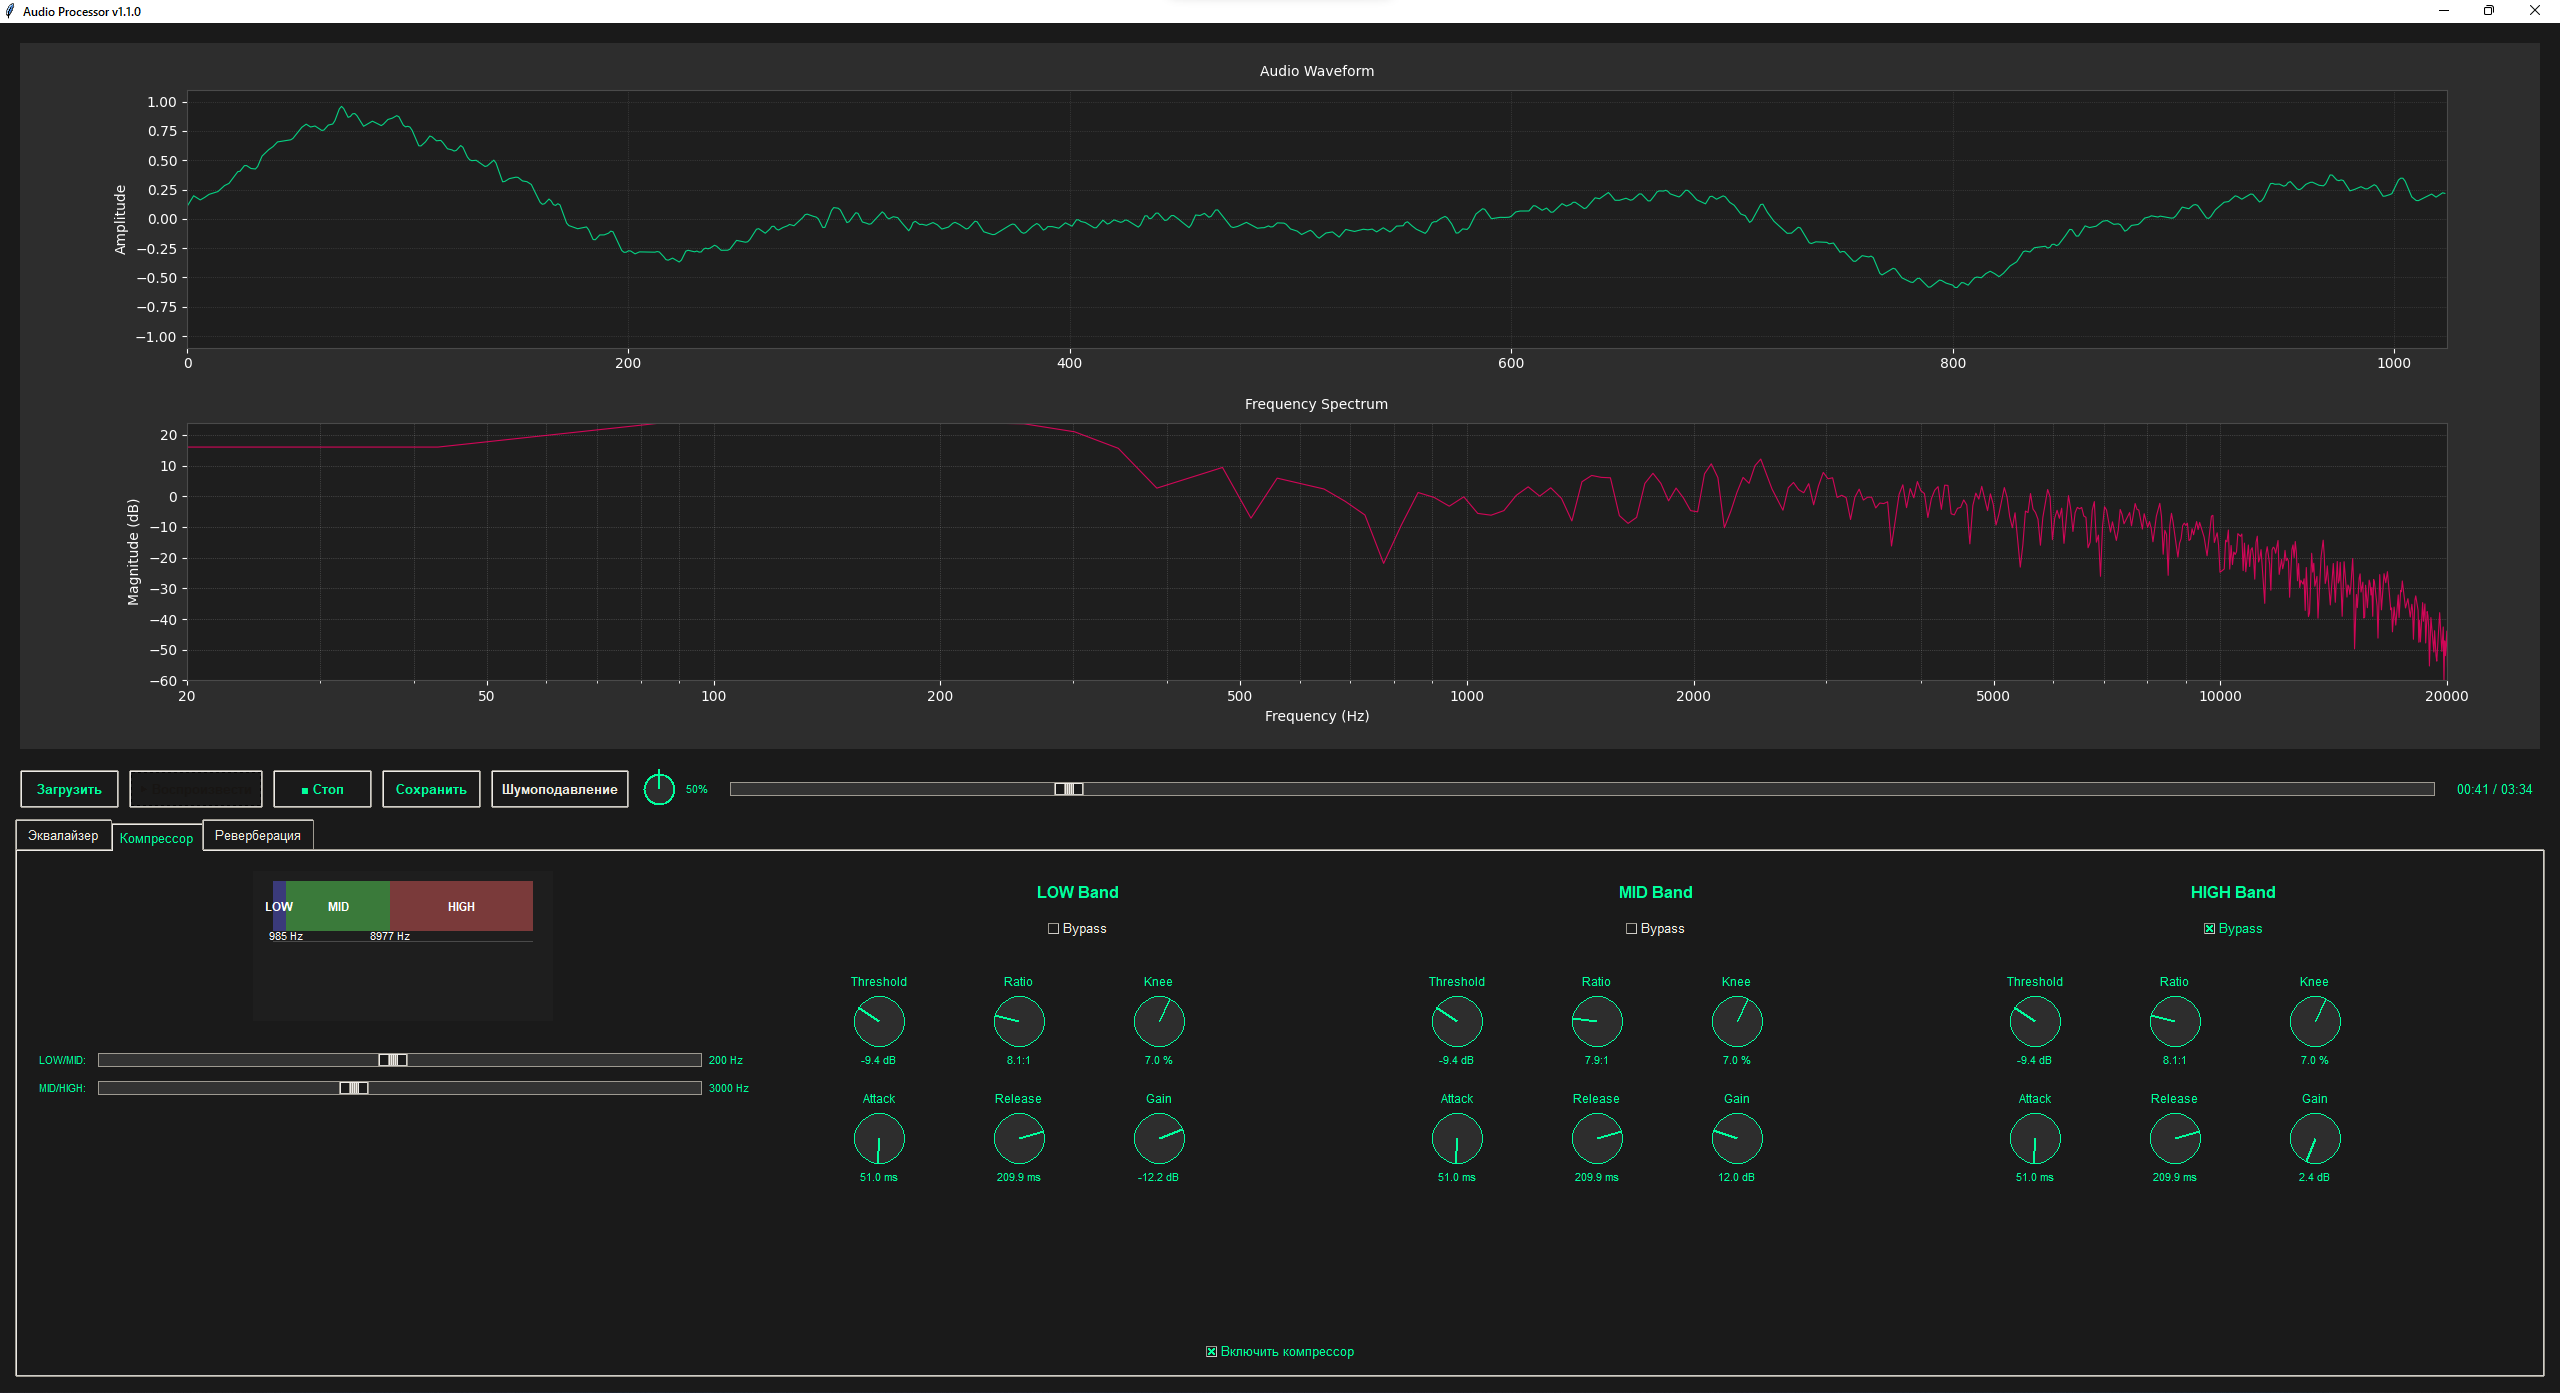
\includegraphics[width=0.8\linewidth]{CompParam}}
	\caption{Изменение параметров компрессора.}
	\label{CompParam:image}
\end{figure}

На рисунке \ref{CompParamOff:image} отображение графиков при выключенном компрессоре.

\begin{figure}[ht]
	\center{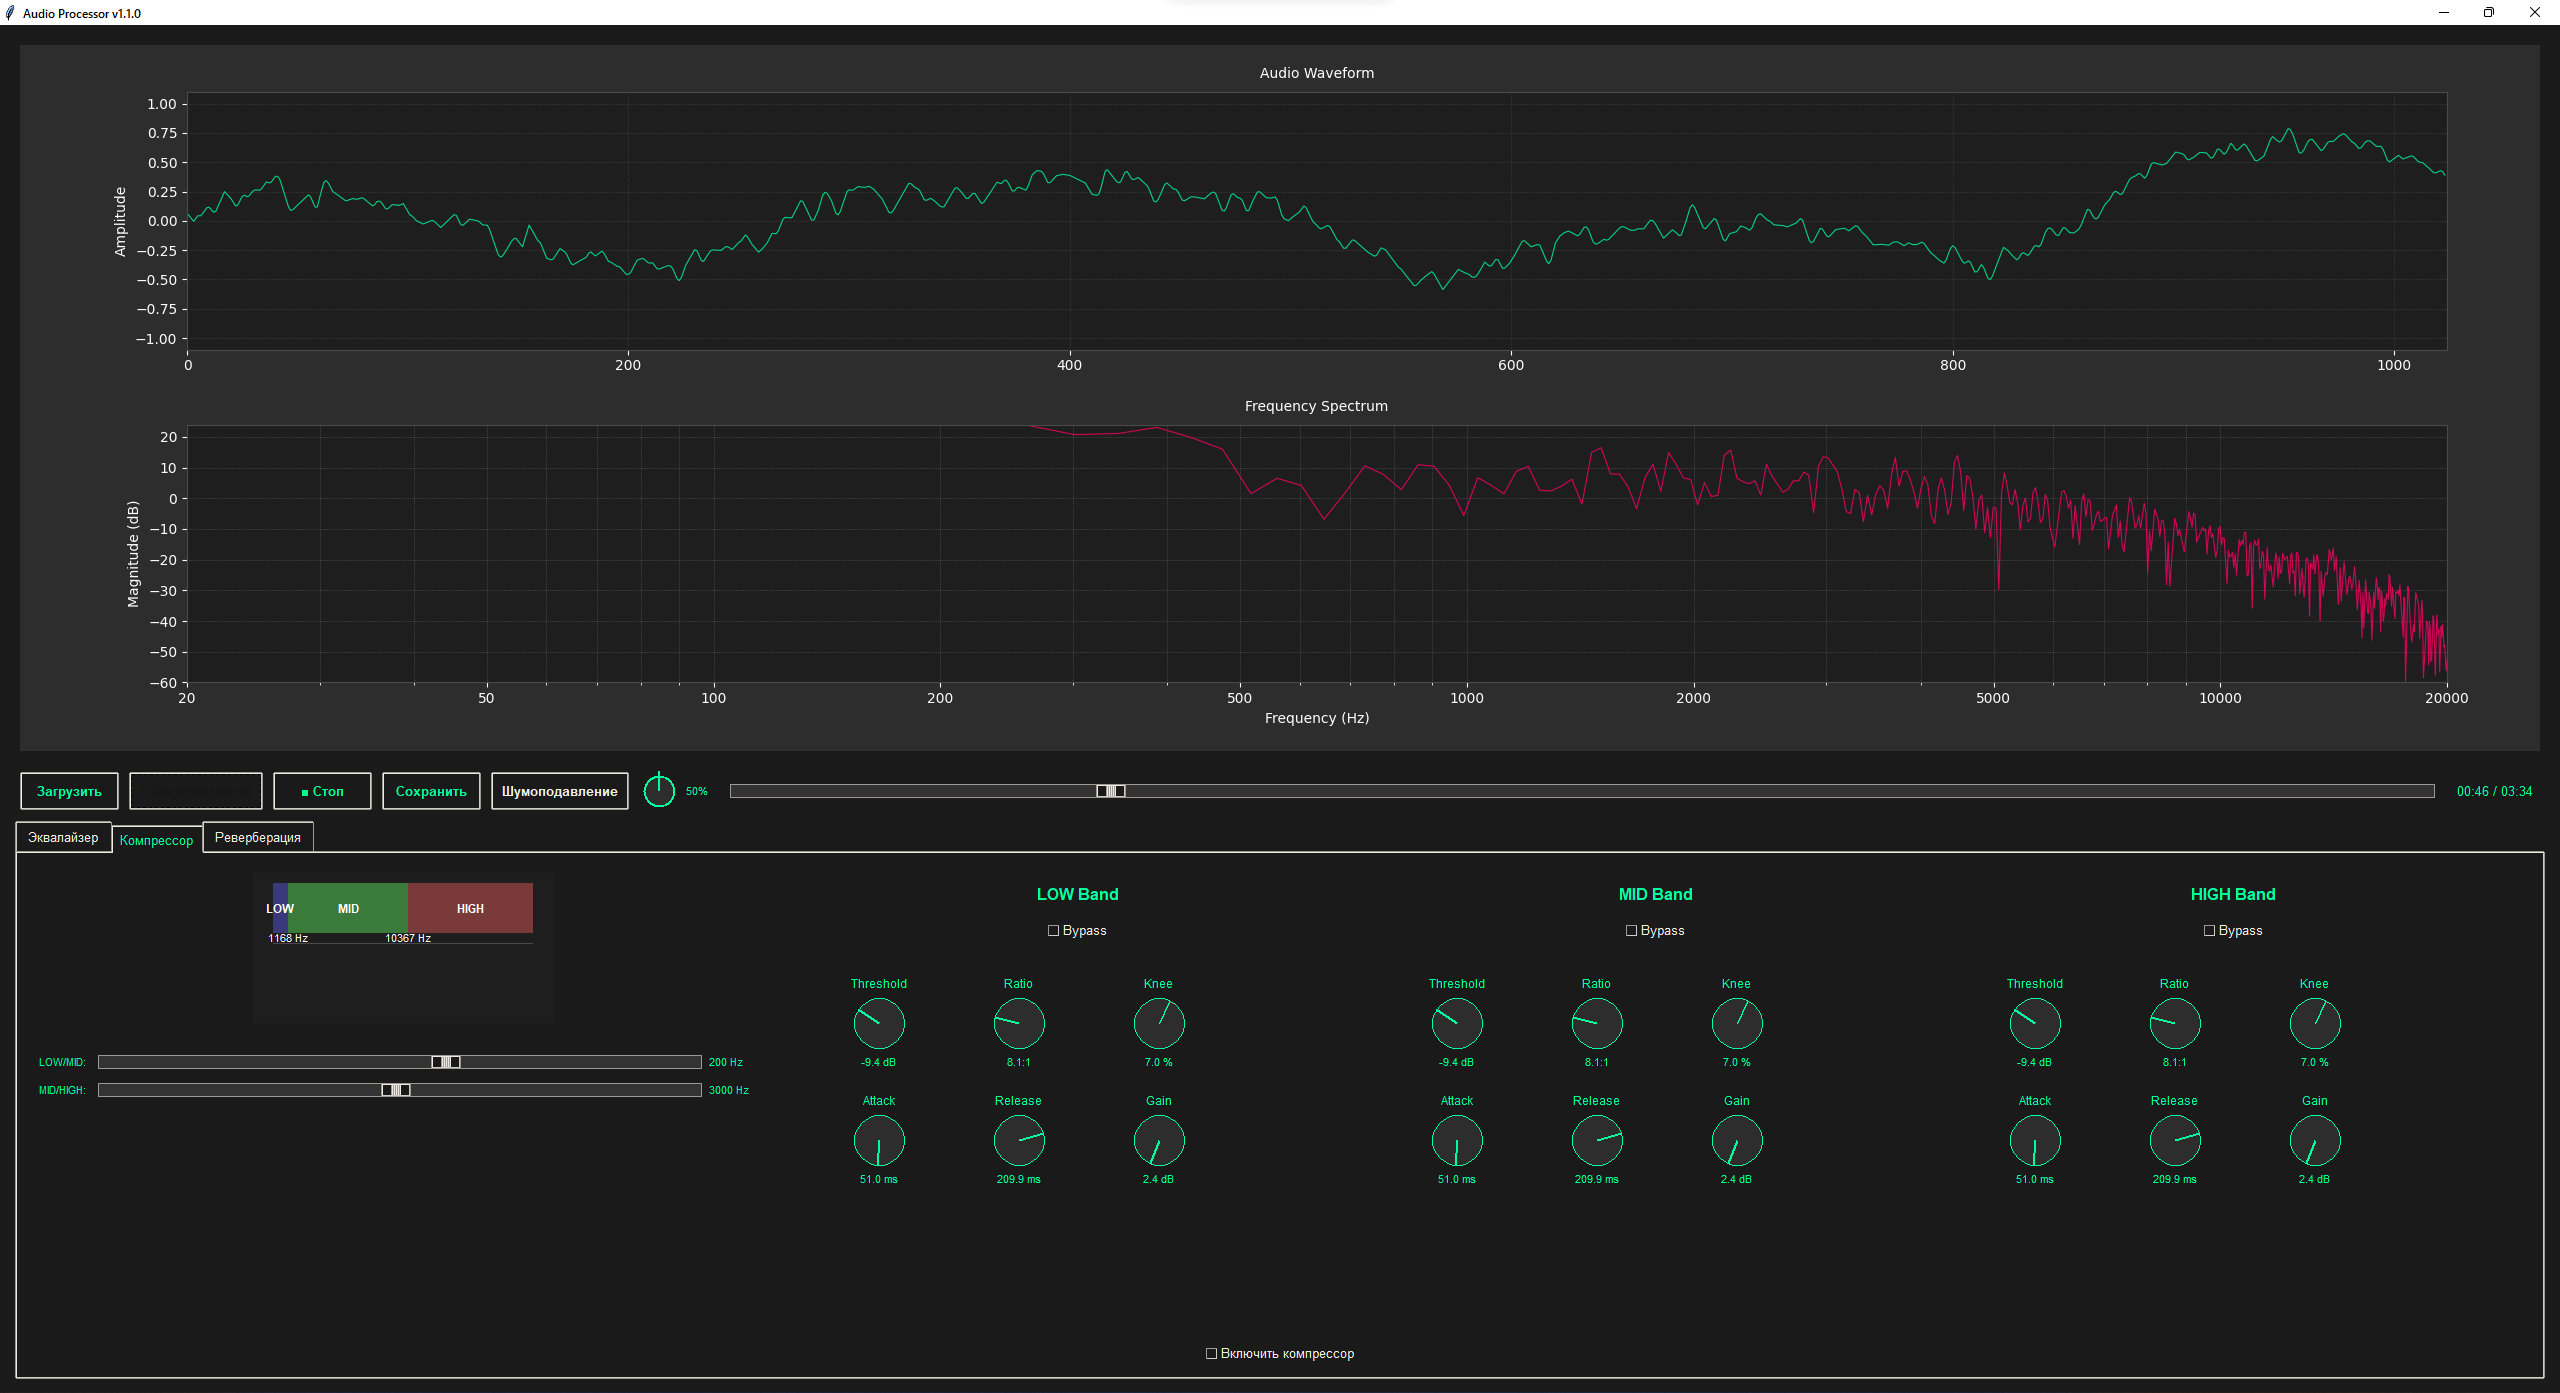
\includegraphics[width=0.8\linewidth]{CompParamOff}}
	\caption{Отображение графиков при выключенном компрессоре.}
	\label{CompParamOff:image}
\end{figure}
\clearpage

\textbf{7) Изменение параметров реверберации}

Описание: При изменении параметров реверберации, регулировки knob, все изменения применяются сразу, без задержек и прерываний. Так же изменяются графики формы волны и АЧХ.

На рисунке \ref{ReverbParam:image} изменение параметров компрессора.

\begin{figure}[ht]
	\center{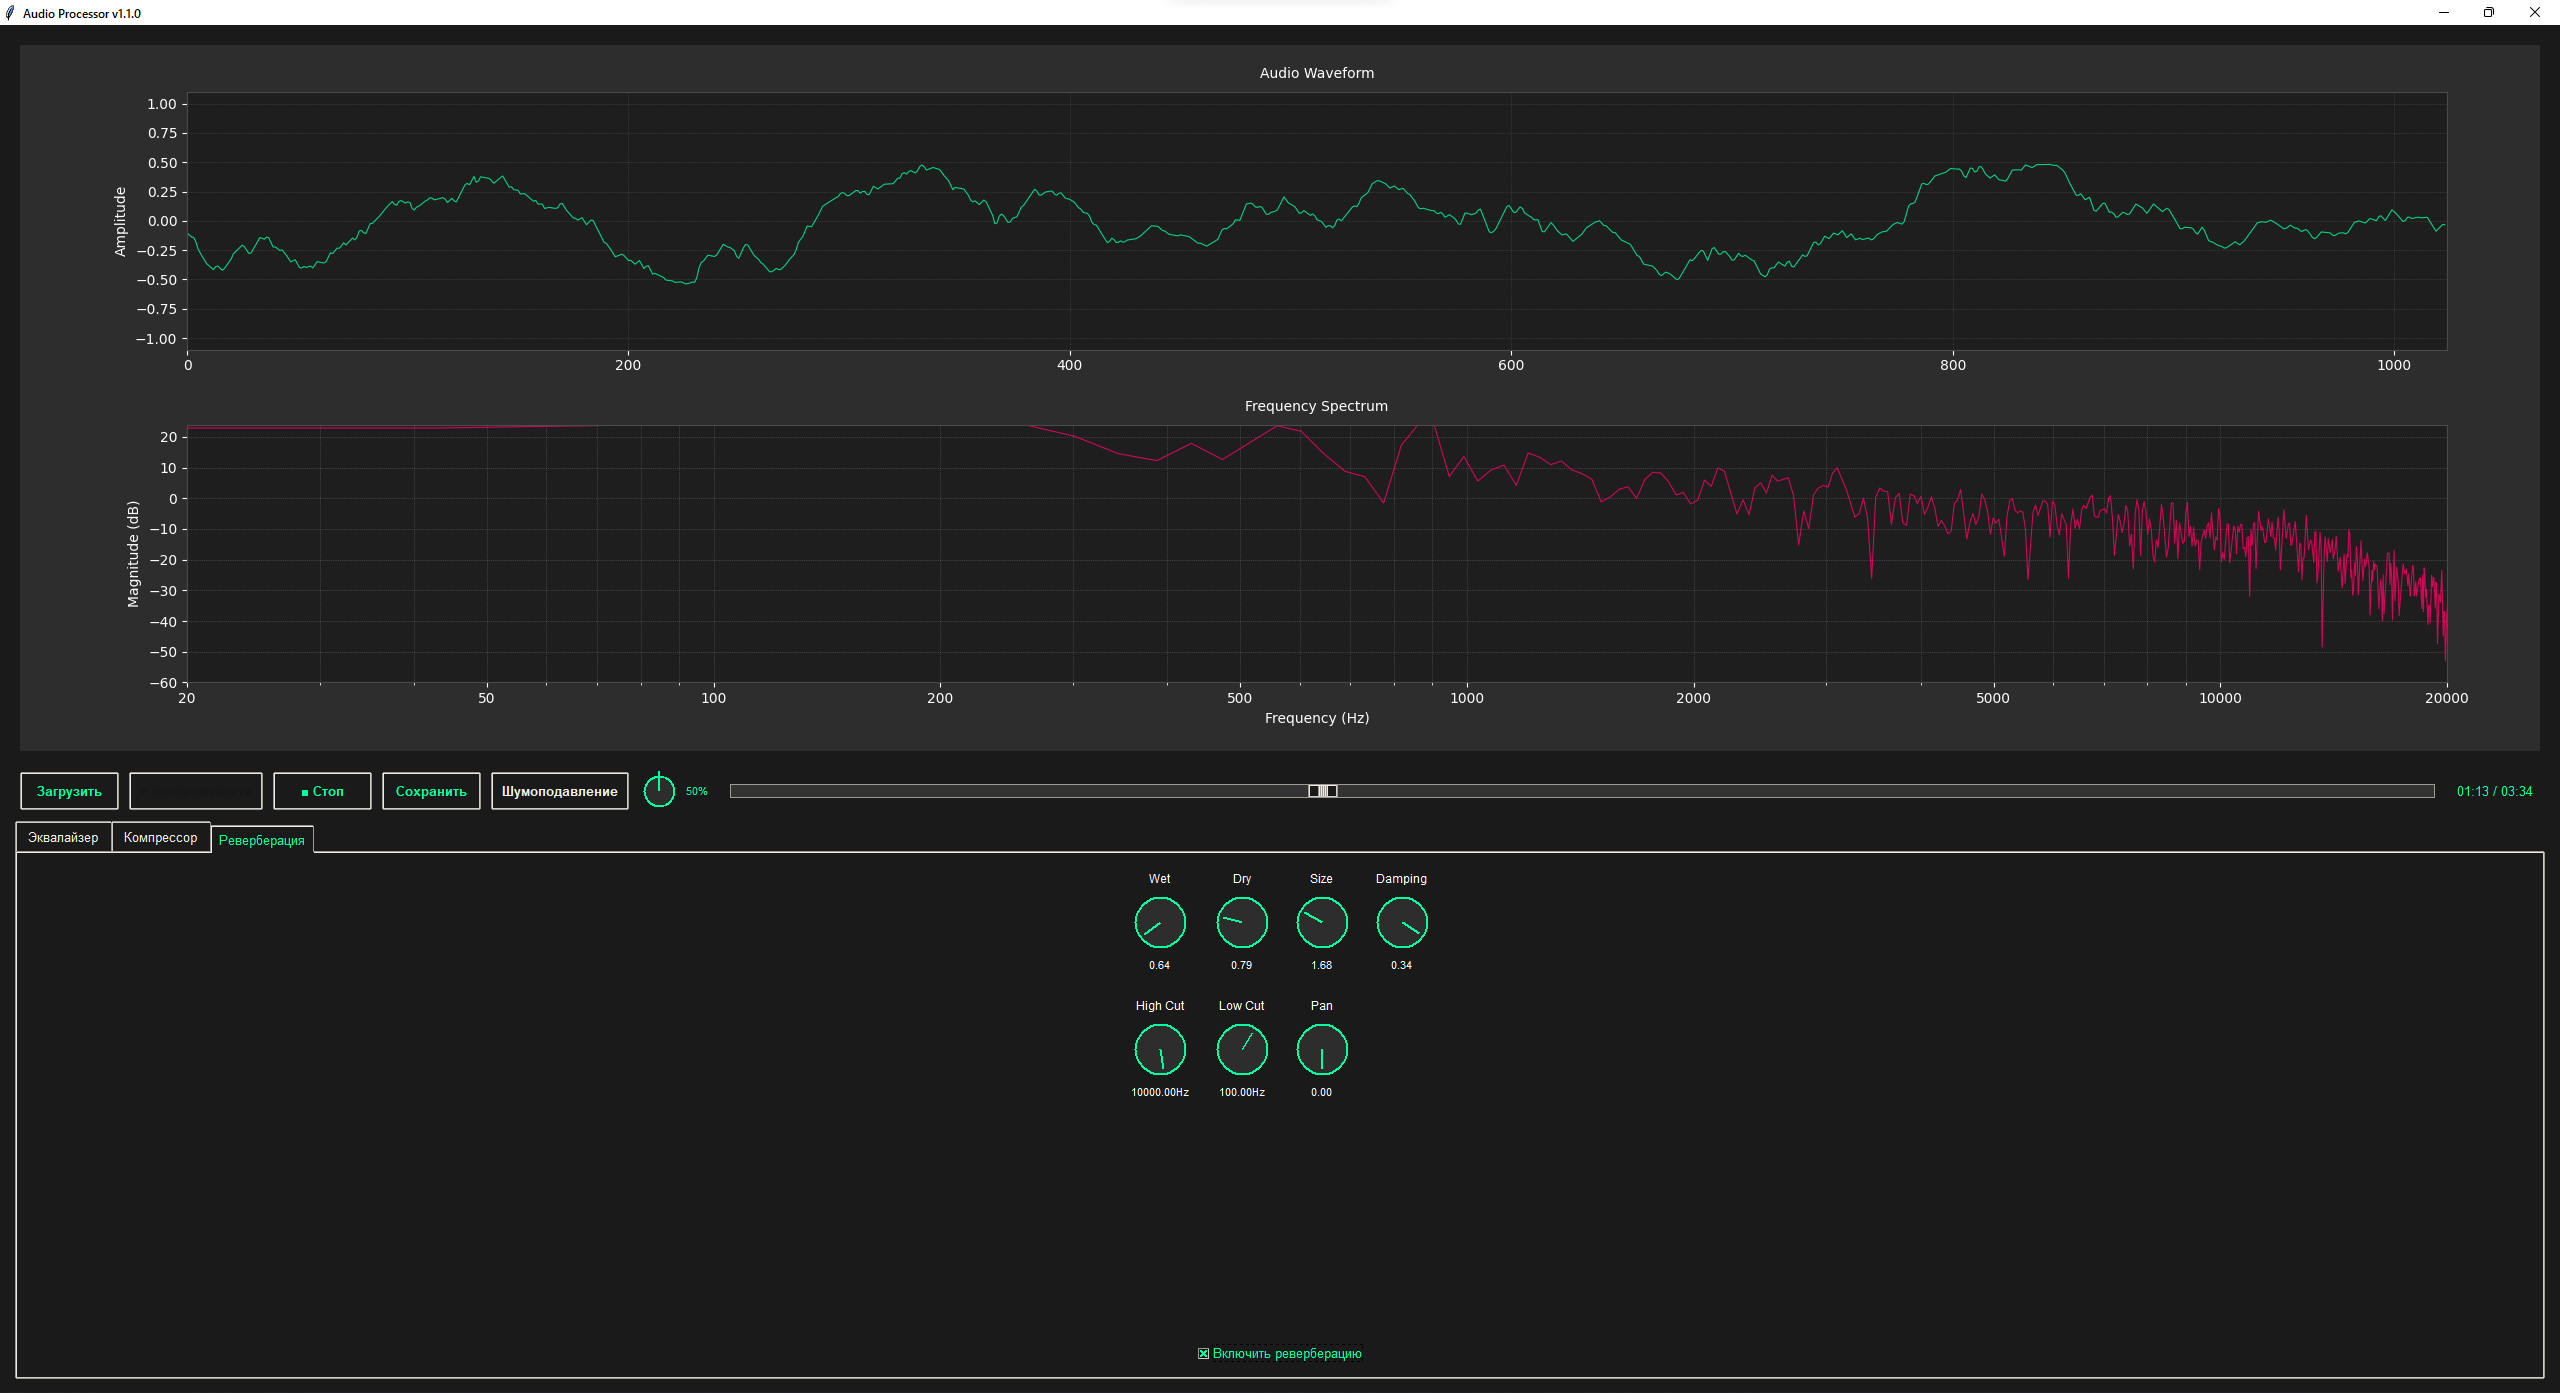
\includegraphics[width=0.8\linewidth]{ReverbParam}}
	\caption{Изменение параметров реверберации.}
	\label{ReverbParam:image}
\end{figure}

На рисунке \ref{ReverbParamOff:image} отображение графиков при выключенной ревереберации.

\begin{figure}[ht]
	\center{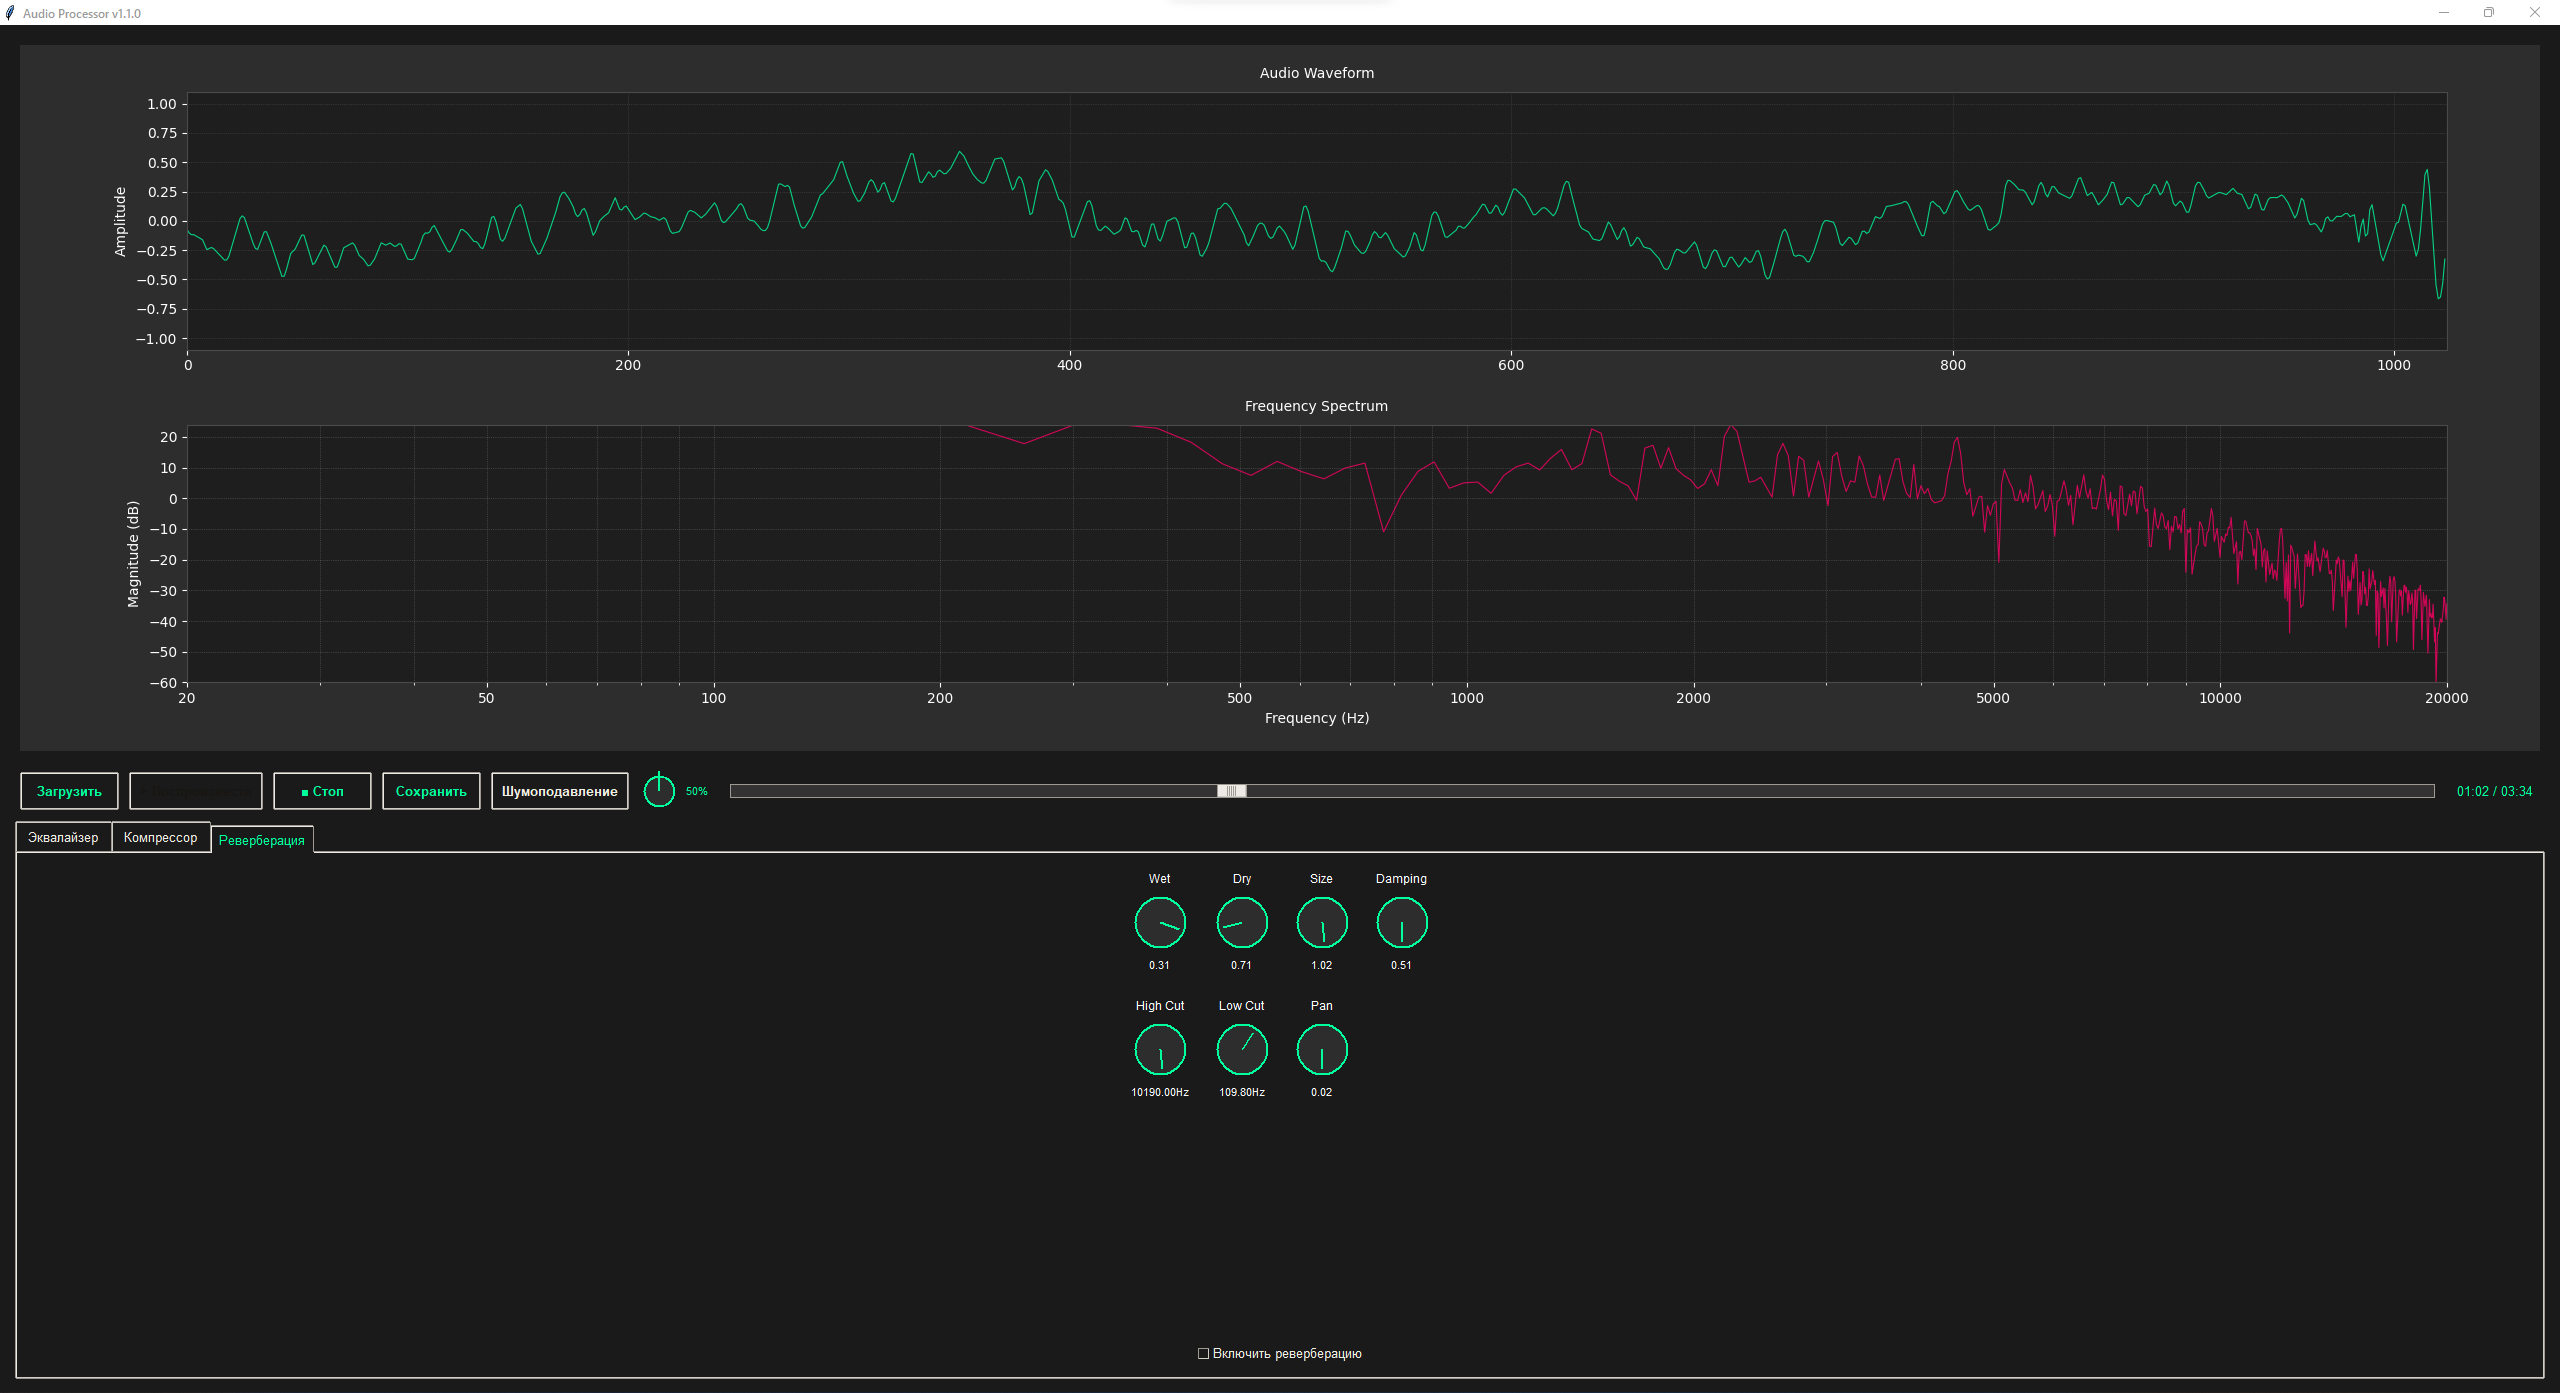
\includegraphics[width=0.8\linewidth]{ReverbParamOff}}
	\caption{Отображение графиков при выключенной реверберации.}
	\label{ReverbParamOff:image}
\end{figure}
\clearpage


   \section*{ЗАКЛЮЧЕНИЕ}
\addcontentsline{toc}{section}{ЗАКЛЮЧЕНИЕ}

В ходе выполнения данной дипломной работы был разработа программный аудиопроцессор на языке Python, способный выполнять многополосную обработку аудиосигнала в реальном времени с применением современных эффектов, таких как компрессия, эквализация, реверберация и шумоподавление. В процессе работы был создан модуль архитектуры, произведена оптимизация производительности и реализована возможность гибкой настройки параметров обработки.

Задачи, поставленные в начале разработки были решены следующим образом:
\begin{itemize}
	\item разработаны оптимальные алгоритмы реализации шумоподавления, эквализации, компрессии и реверберации;
	\item спроектирована архитектура программной системы, обеспечивающая модульность, расширяемость и эффективность взаимодействия всех компонентов;
	\item реализован модуль обработки и воспроизведения аудиосигнала с поддержкой работы в реальном времени;
	\item создан удобный и понятный интерфейс приложения с отображением графиков формы волны и АЧХ.
\end{itemize}

Особое внимание уделялось оптимизации производительности с использованием технологий JIT-компиляции (Numba) и многопоточности, что позволило обеспечить обработку аудиосигнала в реальном времени с минимальной задержкой. Разработанный аудиопроцессор продемонстрировал высокое качество звуковой обработки, гибкость настройки параметров и устойчивость к ошибкам.

Результаты работы могут быть использованы как основа для дальнейшего развития программных аудиопроцессоров, расширения функционала и интеграции с другими аудиосистемами. Практическая значимость проекта заключается в создании универсального инструмента для динамической обработки звука, который может применяться в профессиональной звукозаписи, радиовещании, а также в бытовых аудиоприложениях.

Таким образом, поставленные цели и задачи дипломной работы полностью достигнуты, а разработанная система соответствует современным требованиям к качеству и эффективности цифровой обработки аудиосигналов.
}\fi
\addcontentsline{toc}{section}{СПИСОК ИСПОЛЬЗОВАННЫХ ИСТОЧНИКОВ}

\begin{thebibliography}{9}
	
	\bibitem{DSP} Витязев В.В., Волченков В.А. Цифровая обработка сигналов – Москва: Лань, 2023 – 448 с., ISBN 978-5-8114-5804-9 – Текст: непосредственный.
	\bibitem{DSP} Шиндор О.В., Чикрин Д.Е., Кокунин П.А. Цифровая обработка сигналов – Москва: Лань, 2025 – 400 с., ISBN 978-5-8114-5810-0 – Текст: непосредственный
	\bibitem{DSP} Григорьев Д.Л. Цифровая обработка аудиосигналов / Д.Л. Григорьев – Москва: ДМК Пресс, 2018 – 352 с., ISBN 978-5-97060-670-6 – Текст: непосредственный.
	\bibitem{python} Брайан Джонс, Тиан Чжан. Python. Карманный справочник / Brian Jones, Tiaan Chan – Санкт-Петербург: Питер, 2021 – 320 с., ISBN 978-5-4461-1640-7 – Текст: непосредственный.
	\bibitem{python} Брайан Кинг. Python и обработка аудиосигналов / King B. – Москва: ДМК Пресс, 2020 – 288 с., ISBN 978-5-97060-960-8 – Текст: непосредственный.
	\bibitem{DSP} Кузнецов Ю.А. Теория и практика цифровой обработки сигналов – Москва: Горячая линия – Телеком, 2015 – 368 с., ISBN 978-5-9912-0575-6 – Текст: непосредственный.
	\bibitem{DSP} Блинов М.И. Программирование цифровых фильтров – Санкт-Петербург: Питер, 2018 – 224 с., ISBN 978-5-4461-1278-2 – Текст: непосредственный.
	\bibitem{python} Громов В.А. Программирование аудиоприложений на Python – Санкт-Петербург: Питер, 2022 – 256 с., ISBN 978-5-4461-1642-1 – Текст: непосредственный.
	\bibitem{DSP} Капустин С.А. Теория и практика цифровой фильтрации – Москва: Физматлит, 2017 – 296 с., ISBN 978-5-9221-1767-2 – Текст: непосредственный.
	\bibitem{python} Кулагин В.П. Программирование на Python для инженеров – Москва: ДМК Пресс, 2020 – 320 с., ISBN 978-5-97060-960-8 – Текст: непосредственный
	\bibitem{DSP} Тихонов А.Н. Аудиообработка в мультимедийных приложениях - М.: Горячая линия-Телеком, 2021 - 408 с., ISBN 978-5-9912-0791-0 - Текст: непосредственный.
	\bibitem{DSP} Васнецов П.А. Программирование аудиоэффектов на Python - Екатеринбург: УрФУ, 2022 - 276 с., ISBN 978-5-321-02497-3 - Текст: непосредственный.
	\bibitem{DSP} Семенов А.Ю. Реализация аудиоэффектов на языке Python - Москва: ДМК Пресс, 2022 - 352 с., ISBN 978-5-93700-107-8 - Текст: непосредственный.
	\bibitem{DSP} Федоров Р.А. Эквалайзеры и фильтры в аудиоприложениях - Новосибирск: НГТУ, 2019 - 212 с., ISBN 978-5-7782-3784-9 - Текст: непосредственный.
	\bibitem{DSP} Волков Л.А. Реверберация и пространственная обработка звука - Санкт-Петербург.: Лань, 2017 - 320 с., ISBN 978-5-8114-2452-3 - Текст: непосредственный.
	\bibitem{DSP} Николаев А.Г., Соколов Е.В. Алгоритмы компрессии аудиосигналов - Москва: Радио и связь, 2018 - 256 с., ISBN 978-5-256-01987-6 - Текст: непосредственный.
	\bibitem{DSP} Гришин В.О. Цифровые аудиоэффекты: теория и реализация - Москва: Горячая линия-Телеком, 2019 - 364 с., ISBN 978-5-9912-0729-3 - Текст: непосредственный
	\bibitem{DSP} Иванов П.К. Современные методы цифровой обработки звука - Москва: Техносфера, 2020 - 416 с., ISBN 978-5-94836-567-1 - Текст: непосредственный.
	\bibitem{DSP} Смирнов Д.А., Козлов С.В. Алгоритмы шумоподавления в аудиосистемах - Москва: ДМК Пресс, 2019 - 288 с., ISBN 978-5-97060-689-4 - Текст: непосредственный.
	\bibitem{DSP} Соколов Д.В. Многопоточная обработка аудиосигналов - Москва: Радио и связь, 2021 - 320 с., ISBN 978-5-256-02245-6 - Текст: непосредственный.
	
\end{thebibliography}

\ifВКР{\appendix{Представление графического материала}

Графический материал, выполненный на отдельных листах,
изображен на рисунках А.1--А.\arabic{числоПлакатов}.
\setcounter{числоПлакатов}{0}

\renewcommand{\thefigure}{А.\arabic{figure}} % шаблон номера для плакатов

\begin{landscape}

\begin{плакат}
	\includegraphics[width=0.82\linewidth,page=1]{plac1.png}
	\заголовок{Сведения о ВКРБ}
	\label{plac1:image}      
\end{плакат}

\begin{плакат}
	\includegraphics[width=0.82\linewidth,page=2]{plac2.png}
	\заголовок{Цели и задачи разработки}
	\label{plac2:image}      
\end{плакат}


\begin{плакат}
	\includegraphics[width=0.82\linewidth,page=3]{plac3.png}
	\заголовок{Диаграмма прецедентов}
	\label{plac3:image}      
\end{плакат}


\begin{плакат}
	\includegraphics[width=0.82\linewidth,page=4]{plac4.png}
	\заголовок{Архитектура приложения}
	\label{plac4:image}      
\end{плакат}


\begin{плакат}
	\includegraphics[width=0.82\linewidth,page=5]{plac5.png}
	\заголовок{Интерфейс программы}
	\label{plac5:image}      
\end{плакат}


\begin{плакат}
	\includegraphics[width=0.82\linewidth,page=6]{plac6.png}
	\заголовок{Интерфейс вкладки компрессора и графиков}
	\label{plac6:image}      
\end{плакат}


\begin{плакат}
	\includegraphics[width=0.82\linewidth,page=7]{plac7.png}
	\заголовок{Интерфейс вкладки реверберации и графиков}
	\label{plac7:image}      
\end{плакат}

\begin{плакат}
	\includegraphics[width=0.82\linewidth,page=8]{plac8.png}
	\заголовок{Заключение}
	\label{plac8:image}      
\end{плакат}

\end{landscape}
}\fi
\ifПрактика{}\else{\appendix{Фрагменты исходного кода программы}

main.tex
\lstinputlisting[language=Tex, frame=none]{main.tex}

ТехПроект.tex
\lstinputlisting[language=Tex, frame=none]{ТехПроект.tex}

\ifВКР{
\newpage
\addcontentsline{toc}{section}{На отдельных листах (CD-RW в прикрепленном конверте)}
\noindent
\begin{tabular}{p{5.8cm}C{4.8cm}C{4.8cm}}
   Автор ВКР & \lhrulefill{\fill} & \fillcenter\Автор \\
            \setarstrut{\footnotesize}
           & \footnotesize{(подпись, дата)} & \\
            \restorearstrut
   Руководитель ВКР & \lhrulefill{\fill} & \fillcenter\Руководитель \\
            \setarstrut{\footnotesize}
           & \footnotesize{(подпись, дата)} & \\
            \restorearstrut
   Нормоконтроль & \lhrulefill{\fill} & \fillcenter\Нормоконтроль \\
            \setarstrut{\footnotesize}
           & \footnotesize{(подпись, дата)} & \\
            \restorearstrut
\end{tabular}
\vskip 2cm
\begin{center}
\textbf{Место для диска}
\end{center}
}\fi
}\fi
\end{document}
